%%%%%%%% ICML 2022 EXAMPLE LATEX SUBMISSION FILE %%%%%%%%%%%%%%%%%

\documentclass[nohyperref]{article}

% Robust UTF-8 names/affiliations across pdfTeX/Tectonic/MiKTeX setups.
\usepackage[T1]{fontenc}
\usepackage[utf8]{inputenc}

% Recommended, but optional, packages for figures and better typesetting:
\usepackage{microtype}
\usepackage{graphicx}
\usepackage{booktabs} % for professional tables

% hyperref makes hyperlinks in the resulting PDF.
% If your build breaks (sometimes temporarily if a hyperlink spans a page)
% please comment out the following usepackage line and replace
% \usepackage{icml2022} with \usepackage[nohyperref]{icml2022} above.
\usepackage{hyperref}


% Attempt to make hyperref and algorithmic work together better:
\newcommand{\theHalgorithm}{\arabic{algorithm}}

% Use the following line for the initial blind version submitted for review:
%\usepackage{icml2022}

% If accepted, instead use the following line for the camera-ready submission:
\usepackage[accepted]{icml2022}

% For theorems and such
\usepackage{amsmath}
\usepackage{amssymb}
\usepackage{mathtools}
\usepackage{amsthm}
\usepackage{calligra}
\usepackage{graphicx}
\usepackage{subcaption}
\usepackage{cuted}  

% if you use cleveref..
\usepackage[capitalize,noabbrev]{cleveref}

%%%%%%%%%%%%%%%%%%%%%%%%%%%%%%%%
% THEOREMS
%%%%%%%%%%%%%%%%%%%%%%%%%%%%%%%%
\theoremstyle{plain}
\newtheorem{theorem}{Theorem}[section]
\newtheorem{proposition}[theorem]{Proposition}
\newtheorem{lemma}[theorem]{Lemma}
\newtheorem{corollary}[theorem]{Corollary}
\theoremstyle{definition}
\newtheorem{definition}[theorem]{Definition}
\newtheorem{assumption}[theorem]{Assumption}
\theoremstyle{remark}
\newtheorem{remark}[theorem]{Remark}

% Todonotes is useful during development; simply uncomment the next line
%    and comment out the line below the next line to turn off comments
%\usepackage[disable,textsize=tiny]{todonotes}
\usepackage[textsize=tiny]{todonotes}
\usetikzlibrary{arrows.meta}


% The \icmltitle you define below is probably too long as a header.
% Therefore, a short form for the running title is supplied here:
\icmltitlerunning{On the Separation of Harmfulness and Refusal in Reasoning Language Models}

\begin{document}

\twocolumn[
\icmltitle{On the Separation of Harmfulness and Refusal in Reasoning Language Models}

\icmlsetsymbol{equal}{*}

\begin{icmlauthorlist}
\icmlauthor{Martín López De Ipiña}{equal,yyy}
\icmlauthor{Baisu Zhou}{equal,yyy}
\icmlauthor{Tài Thái}{equal,yyy}
\end{icmlauthorlist}

\icmlaffiliation{yyy}{Department of Computer Science, University of Tübingen, Tübingen, Germany}

\icmlcorrespondingauthor{Martín López De Ipiña}{martin.lopezdeipina@student.uni-tuebingen.de}
\icmlcorrespondingauthor{Baisu Zhou}{baisu.zhou@student.uni-tuebingen.de}
\icmlcorrespondingauthor{Tài Thái}{tai.thai@student.uni-tuebingen.de}

\icmlkeywords{Machine Learning, ICML}

\vskip 0.3in
]

\printAffiliationsAndNotice{\icmlEqualContribution} % otherwise use the standard text.


\begin{abstract}
Recent work suggests that safety behavior in language models is not governed by a single latent signal: models can encode whether a request is harmful separately from whether they refuse it. We study whether this separation persists in reasoning or ``thinking'' models, where a chain of thought intervenes between the user request and the final answer. We design a harmful and harmless dataset pipeline to test this. Across Qwen3.5 thinking, non-thinking, and stripped-template settings, we conduct multiple activation analyses to separate refusal from harmfulness. The results suggest that although these directions are no longer present at the same positions as in the Instruct models, the same separation is visible at different token positions. However, causal division is yet to be confirmed.

\end{abstract}

\section{Introduction}

Safety-aligned large language models (LLMs) are expected to answer benign requests while refusing harmful ones. Failures in either direction matter: under-refusal creates unsafe compliance, while over-refusal blocks useful benign requests \citep{wang2024surgical, maskey2026overrefusal}. Prior work often assumes that harmfulness is encoded by the
refusal direction \citep{arditi2024refusallanguagemodelsmediated}, but Zhao J. showed that LLMs encode harmfulness and refusal separately in instruct models \citep{zhao2025harmfulness}. We build on this work to design our experiments, and will refer to it throughout the remainder of this paper.

Instruct models are trained to expect a chat template in order to recognize messages; Figure \ref{fig:tokens} illustrates the chat template for different configurations in Qwen3.5 \citep{qwen3.5}. In this setting, the authors define $t_{\text{inst}}$ as the last token of the user query, and $t_{\text{post}}$ as the last token of the prompt tokens. After finding that stripping the $t_{\text{post}}$ token induces 22\% more accepted harmful queries, they conducted several activation analyses to show that the $t_{\text{inst}}$ token's activations encode harmfulness to a greater magnitude, whereas the $t_{\text{post}}$ token encodes refusal to a greater magnitude. It was later demonstrated that the two directions are separated.

\begin{figure*}[h]
\centering
\resizebox{\textwidth}{!}{%
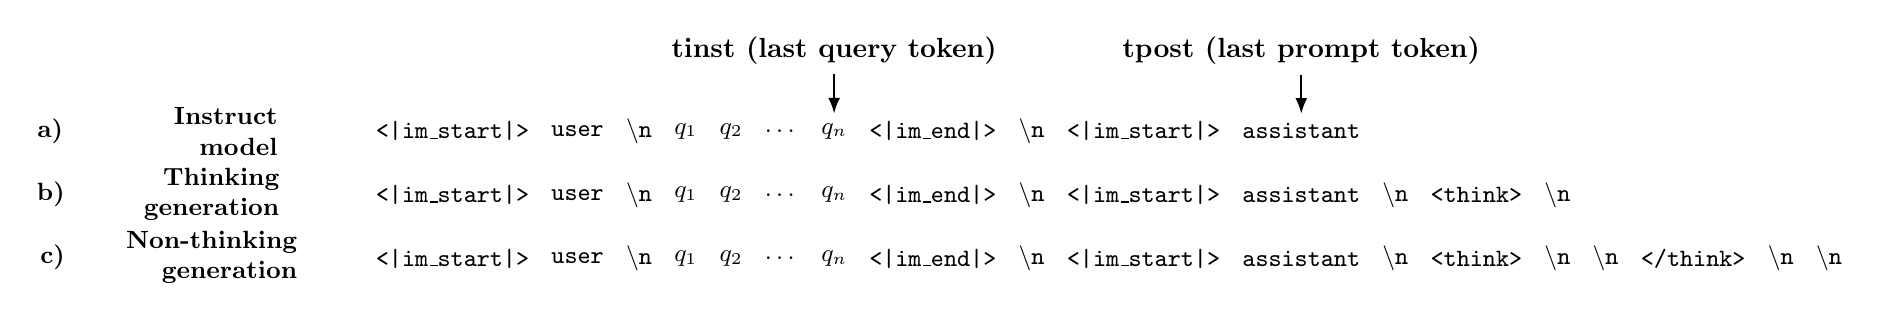
\begin{tikzpicture}[
  tok/.style={font=\ttfamily\small}
]
% Left-side row labels
\node[font=\small\bfseries, align=right] (rowlabel0) at (-1.42,0.8) {Instruct\\model};
\node[font=\small\bfseries, align=right] (rowlabel1) at (-1.6,0) {Thinking\\generation};
\node[font=\small\bfseries, align=right] (rowlabel2) at (-1.6,-0.8) {Non-thinking\\generation};

% a) / b) / c) markers, vertically centered on each two-line label
\node[font=\small\bfseries, right=0.15cm of rowlabel0, anchor=east, xshift=-2.875cm] (marker0) {a)};
\node[font=\small\bfseries, right=0.15cm of rowlabel1, anchor=east, xshift=-2.875cm] (marker1) {b)};
\node[font=\small\bfseries, right=0.15cm of rowlabel2, anchor=east, xshift=-3.1cm] (marker2) {c)};

% Line 1 (new): instruct model, stops at assistant token
\node[tok, right=1cm of rowlabel0, anchor=west] (d1) {<|im\_start|>};
\node[tok, right=1pt of d1] (d2) {user};
\node[tok, right=1pt of d2] (d3) {$\backslash$n};
\node[tok, right=1pt of d3] (dq1) {$q_1$};
\node[tok, right=1pt of dq1] (dq2) {$q_2$};
\node[tok, right=1pt of dq2] (dqdots) {$\dots$};
\node[tok, right=1pt of dqdots] (dqn) {$q_n$};
\node[tok, right=1pt of dqn] (d5) {<|im\_end|>};
\node[tok, right=1pt of d5] (d6) {$\backslash$n};
\node[tok, right=1pt of d6] (d7) {<|im\_start|>};
\node[tok, right=1pt of d7] (d8) {assistant};

\node[font=\normalsize\bfseries, above=0.5 of dqn] (qlabel) {tinst (last query token)};
\draw[-{Latex[length=2mm]}, thick] (qlabel) -- (dqn.north);
\node[font=\normalsize\bfseries, above=0.5 of d8] (plabel) {tpost (last prompt token)};
\draw[-{Latex[length=2mm]}, thick] (plabel) -- (d8.north);

% Line 2: full, up to <think>, with trailing \n
\node[tok, below=23pt of d1.west, anchor=west] (b1) {<|im\_start|>};
\node[tok, right=1pt of b1] (b2) {user};
\node[tok, right=1pt of b2] (b3) {$\backslash$n};
\node[tok, right=1pt of b3] (bq1) {$q_1$};
\node[tok, right=1pt of bq1] (bq2) {$q_2$};
\node[tok, right=1pt of bq2] (bqdots) {$\dots$};
\node[tok, right=1pt of bqdots] (bqn) {$q_n$};
\node[tok, right=1pt of bqn] (b5) {<|im\_end|>};
\node[tok, right=1pt of b5] (b6) {$\backslash$n};
\node[tok, right=1pt of b6] (b7) {<|im\_start|>};
\node[tok, right=1pt of b7] (b8) {assistant};
\node[tok, right=1pt of b8] (b9) {$\backslash$n};
\node[tok, right=1pt of b9] (b10) {<think>};
\node[tok, right=1pt of b10] (b11) {$\backslash$n};

% Line 3: full + closing tokens, \n\n between <think> and </think>, \n\n after </think>
\node[tok, below=23pt of b1.west, anchor=west] (c1) {<|im\_start|>};
\node[tok, right=1pt of c1] (c2) {user};
\node[tok, right=1pt of c2] (c3) {$\backslash$n};
\node[tok, right=1pt of c3] (cq1) {$q_1$};
\node[tok, right=1pt of cq1] (cq2) {$q_2$};
\node[tok, right=1pt of cq2] (cqdots) {$\dots$};
\node[tok, right=1pt of cqdots] (cqn) {$q_n$};
\node[tok, right=1pt of cqn] (c5) {<|im\_end|>};
\node[tok, right=1pt of c5] (c6) {$\backslash$n};
\node[tok, right=1pt of c6] (c7) {<|im\_start|>};
\node[tok, right=1pt of c7] (c8) {assistant};
\node[tok, right=1pt of c8] (c9) {$\backslash$n};
\node[tok, right=1pt of c9] (c10) {<think>};
\node[tok, right=1pt of c10] (c11) {$\backslash$n};
\node[tok, right=1pt of c11] (c11b) {$\backslash$n};
\node[tok, right=1pt of c11b] (c12) {</think>};
\node[tok, right=1pt of c12] (c13) {$\backslash$n};
\node[tok, right=1pt of c13] (c14) {$\backslash$n};

\end{tikzpicture}
}
\caption{Chat template tokenization on Qwen model family for instruct models (a) reasoning models thinking generation (b) and reasoning models non-thinking generation (c).}
\label{fig:tokens}
\end{figure*}

Reasoning models make this picture less straightforward. A thinking model may identify harmfulness early, reason about policy or intent during its CoT, and only later decide how to answer. This raises the question we study: \textbf{does harmfulness/refusal separation still hold in thinking models, and where does refusal live once reasoning tokens are introduced?} 

For this matter, we search in thinking models under two different generation configurations: generation with a reasoning trace and generation without a reasoning trace. Figure \ref{fig:tokens}, rows b and c, show the tokenizer template for these two configurations.

\section{Setup and Datasets}
\label{sec:datasets}

In this section, we describe the datasets and configuration used in our experiments.

We first reproduced the original paper's experiments on Qwen2-7B \citep{qwen2} and Llama3-8B \citep{llama3}. We then ran our experiments on Qwen3.5-9B, using the recommended sampling configuration (see Appendix \ref{ap:confg}). For the judge model, Qwen3.5-4B was used, with few-shot examples containing thinking traces to reduce overthinking \citep{ge2025innatereasoningenoughincontext}.

In order to extract the harmful and refusal activations, we collect 3 datasets containing harmful queries: AdvBench \citep{chen2022should}, SorryBench \citep{xie2025sorrybenchsystematicallyevaluatinglarge} and JailbreakBench (JBB) \citep{chao2024jailbreakbench}, and 2 datasets containing harmless queries: XSTest \citep{röttger2024xstesttestsuiteidentifying} and Alpaca \citep{alpaca}. We then apply the two-step pipeline shown in Figure \ref{fig:datasets}:

\begin{figure*}[t]
\centering

\includegraphics[width=0.75\textwidth]{figures/dataset.png}
\caption{Two-step dataset configuration pipeline for the experiments. The datasets are first subject to a manual bucketing based on thinking or non-thinking generation, and then classified using a programmatic and later LLM-judged approach. Red buckets represent datasets containing harmful queries, whereas green buckets represent datasets containing harmless queries.}
\label{fig:datasets}
\end{figure*}

\textbf{Dataset manual bucketing}. The datasets are first combined according to their behavior (harmful or harmless) and generation configuration (thinking or non-thinking).

\textbf{Response evaluation}. After running the datasets' queries through the model, the generated responses are classified as refused (the model refused to answer due to safety concerns) or accepted (the model answered the query). The responses are first evaluated with a direct match against a common refusal sentence list \citep{zou2023universaltransferableadversarialattacks}. Then, a judge model evaluates only the opposing-behavior buckets, which are more likely to be misclassified (accepted harmful and refused harmless buckets).

Our manual bucketing is based on the following: \emph{(i)} Qwen3.5 has been trained with extensive safety alignment, so unlike in the instruct model experiments, the model refuses almost all queries; we therefore compute a Greedy Coordinate Gradient (GCG) \citep{zou2023universal} jailbreak on the non-thinking generation with an ASR of 34\% using nanoGCG to obtain genuine harmful responses; \emph{(ii)} for the thinking generation, we use SorryBench, which contains soft-harmful queries that violate the model's safety guardrails but might not be as obscene as AdvBench and JBB; \emph{(iii)} for refused harmless responses, we only use XSTest because it contains harmful-looking harmless examples that might trick the model into a refusal.

\section{Experiments and Results}
In this section, we present our approach along with the experiments we conducted. We first test in Section \ref{sec:strip} whether stripping the last tokens also decreases refusal as in Instruct models. Since this proves ineffective, we then search for potential tokens with a strong harmful and refusal signal in Section \ref{sec:activations}. We find that the $t_{post}$ and $t_{gen1}$ tokens encode our desired behavior in the non-thinking configuration. We confirm this in Section \ref{sec:corr} by clustering the buckets in a harmful and refusal score space. In Section \ref{sec:elicit_refusal}, we then steer both directions individually on harmless data points to elicit high refusal rates. We then try the inversion generation experiment proposed by the authors in Section \ref{sec:reply-inversion} to causally prove the direction separation. The results are inconclusive, suggesting that this experiment may not be well suited to these models, which motivates our conclusions.

\subsection{Token stripping generation} \label{sec:strip}
We compare the refusal rate across 4 generation configurations on the AdvBench and JBB datasets. These correspond to the thinking, non-thinking, and two stripped versions. For stripped version A, we only remove the last \texttt{\textbackslash n\textbackslash n} from the non-thinking configuration, which is encoded as a single token. For stripped version B, we strip everything in the thinking configuration up to the <|im\_start|> token. Results are shown in Table \ref{tab:refusal-rate}. Contrary to the Instruct models, none of the configurations shows a decrease in refusal rate.

\begin{table}[h]
\centering
\begin{tabular}{lc}
\hline
\textbf{Generation Configuration} & \textbf{Refusal Rate} \\
\hline
Thinking     & 98.6\% \\
Non-thinking & 98.8\% \\
Strip A      & 97.3\% \\
Strip B      & 98.9\% \\
\hline
\end{tabular}
\caption{Refusal rate by generation configuration.}
\label{tab:refusal-rate}
\end{table}

\subsection{Activation visualization}
\label{sec:activations}

We plot each token's mean activations to search for harmfulness and refusal encoding patterns. Taking the activations for a chosen token, we compute Equation \ref{eq:refusal_score}. We first compute the centroids of the correctly behaved clusters, $\mu_{\text{harmful}}^{\text{refused}}$ and $\mu_{\text{harmless}}^{\text{accepted}}$, using the bucketing explained in Section \ref{sec:datasets}. Then, $s_l$ is defined as the similarity of the mean activations for the chosen token at layer $l$. All the buckets are split into equally sized train and test sets, to ensure that no activation is compared against a mean that contains its own value.


\begin{equation}
\resizebox{0.92\linewidth}{!}{$\displaystyle s_l(h_l) = \text{cos\_sim}\left(h_l, \mu_l^{\text{refused harmful}}\right) - \text{cos\_sim}\left(h_l, \mu_l^{\text{accepted harmless}}\right)$}
\label{eq:refusal_score}
\end{equation}

We use the activations of the opposing expected behavior to test the following hypothesis: if a token's representation is closer to the cluster matching its harmfulness label than to the cluster matching its expected behavior, then that token encodes harmfulness more strongly than refusal, and vice versa. For example, if accepted harmful query activations are closer to the refused harmful centroid, then this token encodes harmfulness to a greater magnitude than refusal; if instead they are closer to the accepted harmless centroid, then the refusal direction is more present. The same logic applies to refused harmless activations.

We run this experiment on the following tokens: \emph{(i)} $t_{inst}$ and $t_{post}$ tokens; \emph{(ii)} \textbackslash n and thinking tag tokens; \emph{(iii)} a set of 15 selected tokens in the CoT: the first 5 tokens of the CoT, the last 5 tokens of the CoT, and 5 selected middle tokens. For the middle tokens, we divide the CoT into 5 groups (excluding the first and last 5) and take the middle index of each group; \emph{(iv)} the first 3 generated tokens.

Figure \ref{fig:grid} shows the results for the distinguished tokens; all the other tokens' plots can be found in the Appendix \ref{ap:plots}. Figure \ref{fig:col_qwen2} shows the desired opposing behavior on Qwen2-7B: tinst encodes harmfulness while tpost encodes refusal. Figure \ref{fig:col_think} and Figure \ref{fig:col_nothink} show the activations for Qwen3.5-9B on thinking and non-thinking generations. Tpost in the non-thinking configuration is the only token among the prompt activations that shows the desired behavior. For this reason, we choose tpost and the first generated token in the non-thinking configuration to continue our experiments. As Figure \ref{fig:col_gen1} shows, we hypothesize that $t_{post}$ contains the harmfulness direction and the first generated token ($t_{gen1}$)  contains the refusal direction.

\begin{figure*}[t]
\centering
\begin{subfigure}[t]{0.24\textwidth}
    \centering
    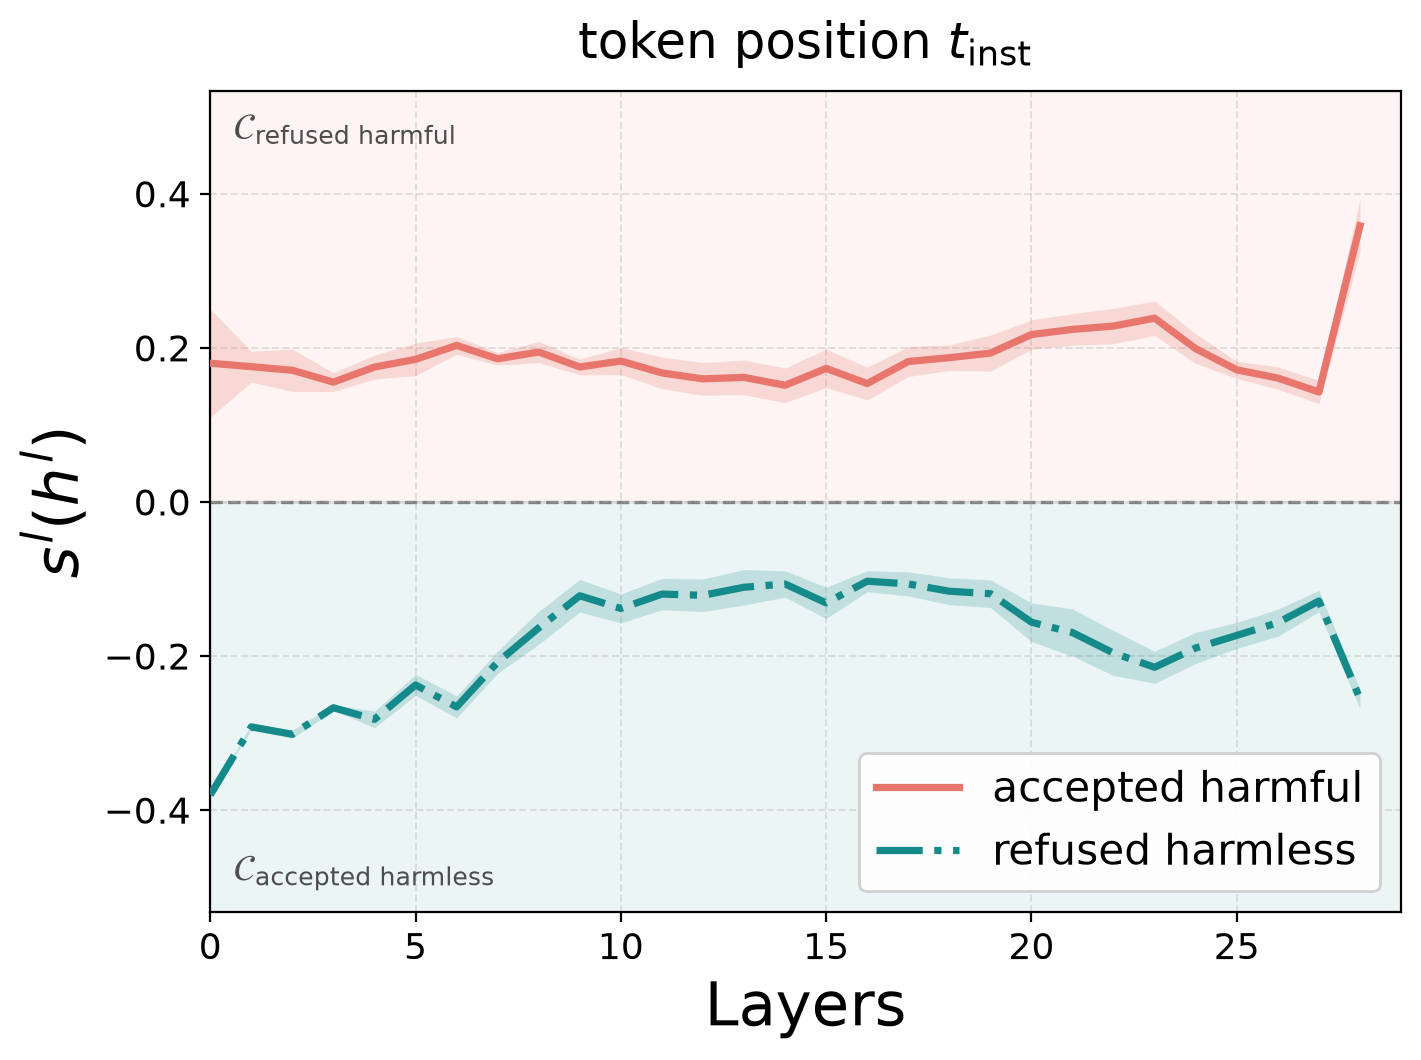
\includegraphics[width=\linewidth]{figures/tinst_qwen2.png}\\[0.3em]
    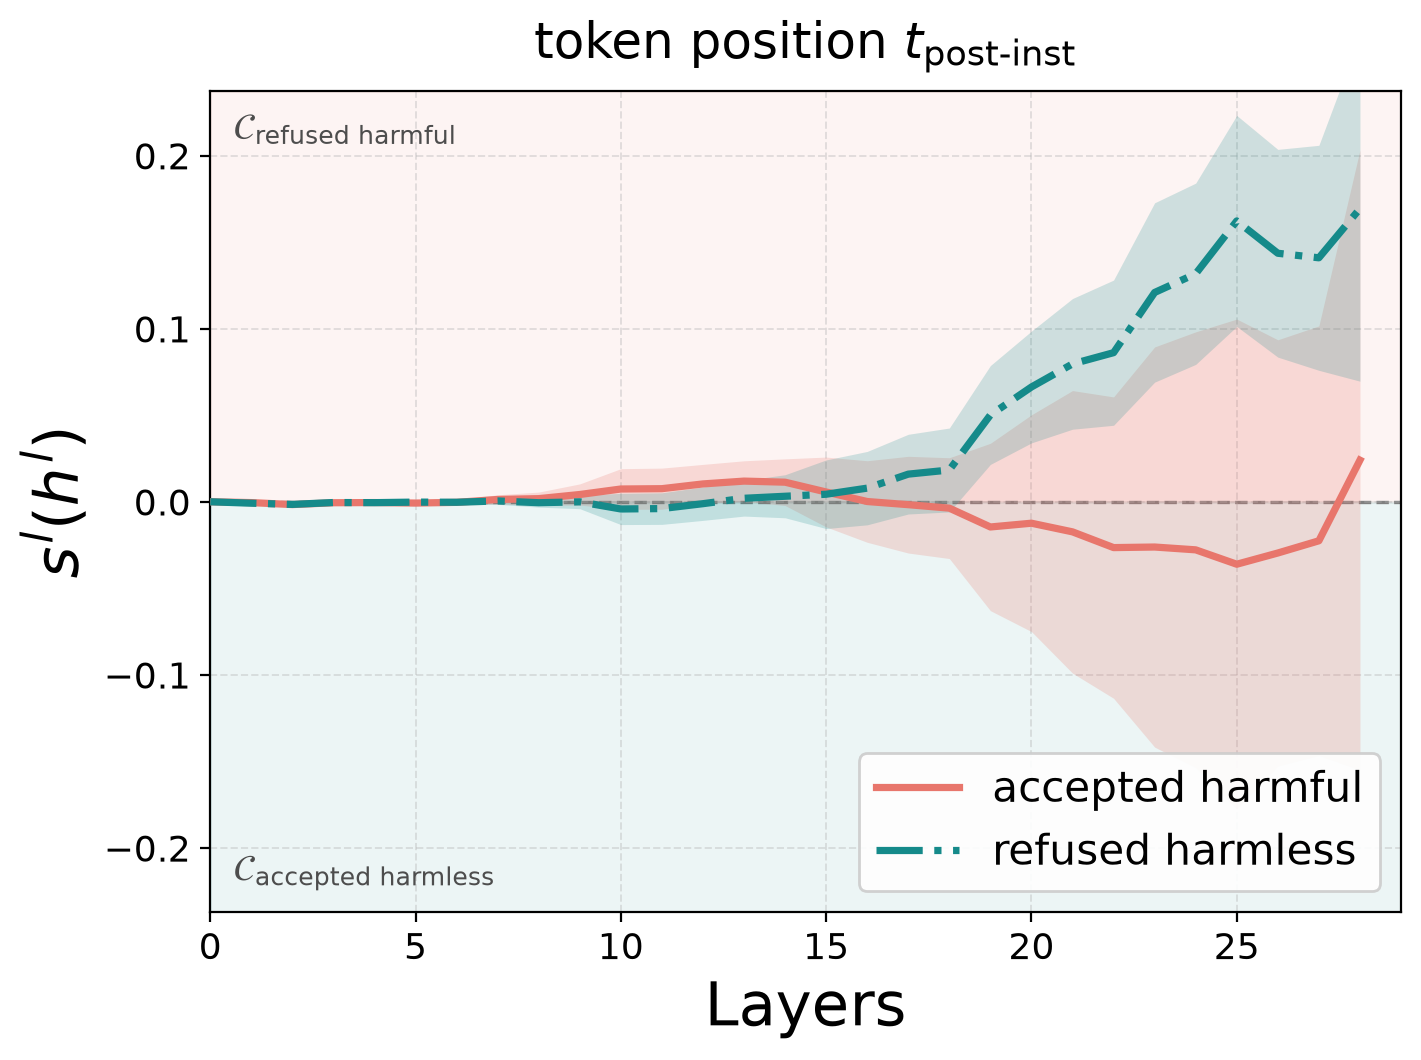
\includegraphics[width=\linewidth]{figures/tpost_qwen2.png}
    \caption{Desired behavior, replicated on Qwen2-7B for tinst and tpost.}
    \label{fig:col_qwen2}
\end{subfigure}
\hfill
\begin{subfigure}[t]{0.24\textwidth}
    \centering
    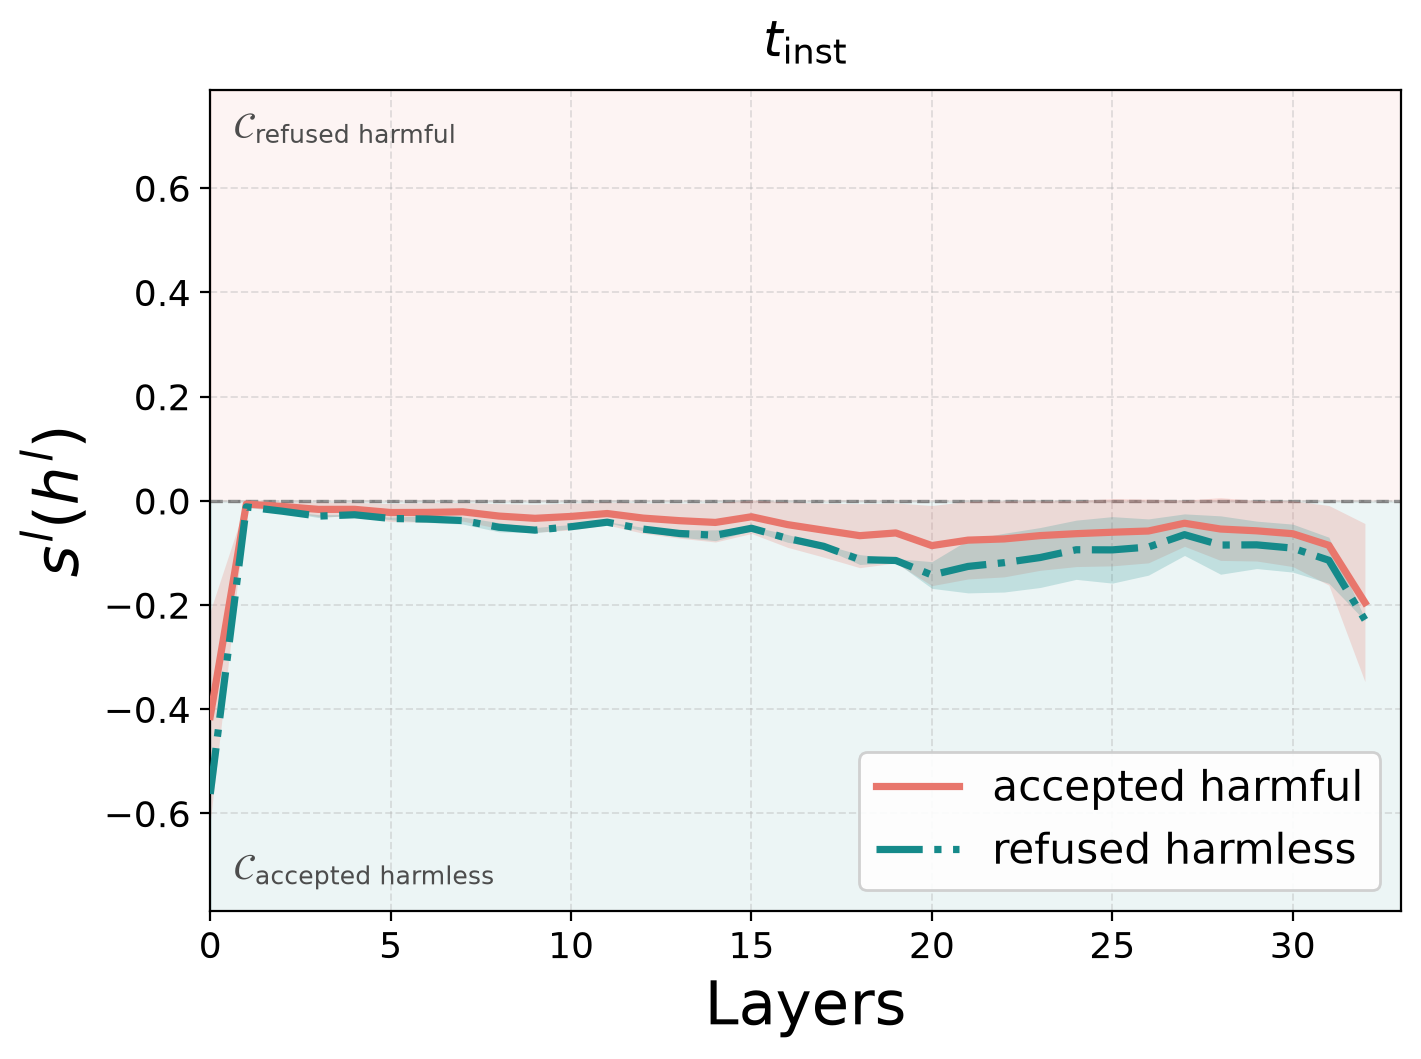
\includegraphics[width=\linewidth]{figures/think_tinst.png}\\[0.3em]
    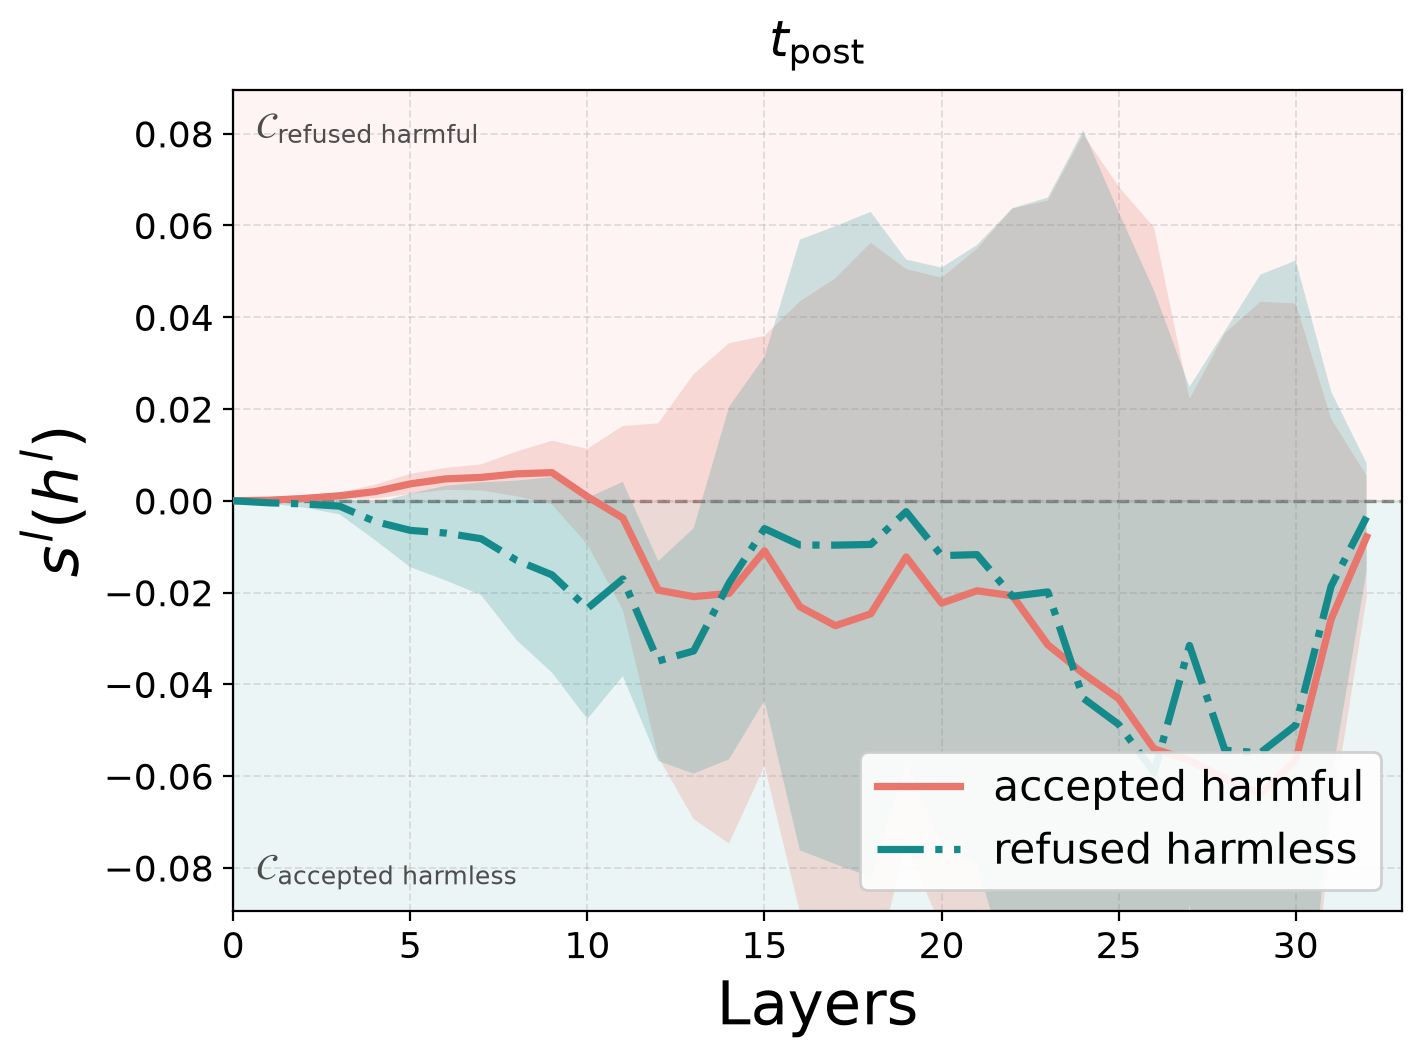
\includegraphics[width=\linewidth]{figures/think_tpost.png}
    \caption{Qwen3.5-9B on thinking configuration, tinst and tpost activations}
    \label{fig:col_think}
\end{subfigure}
\hfill
\begin{subfigure}[t]{0.24\textwidth}
    \centering
    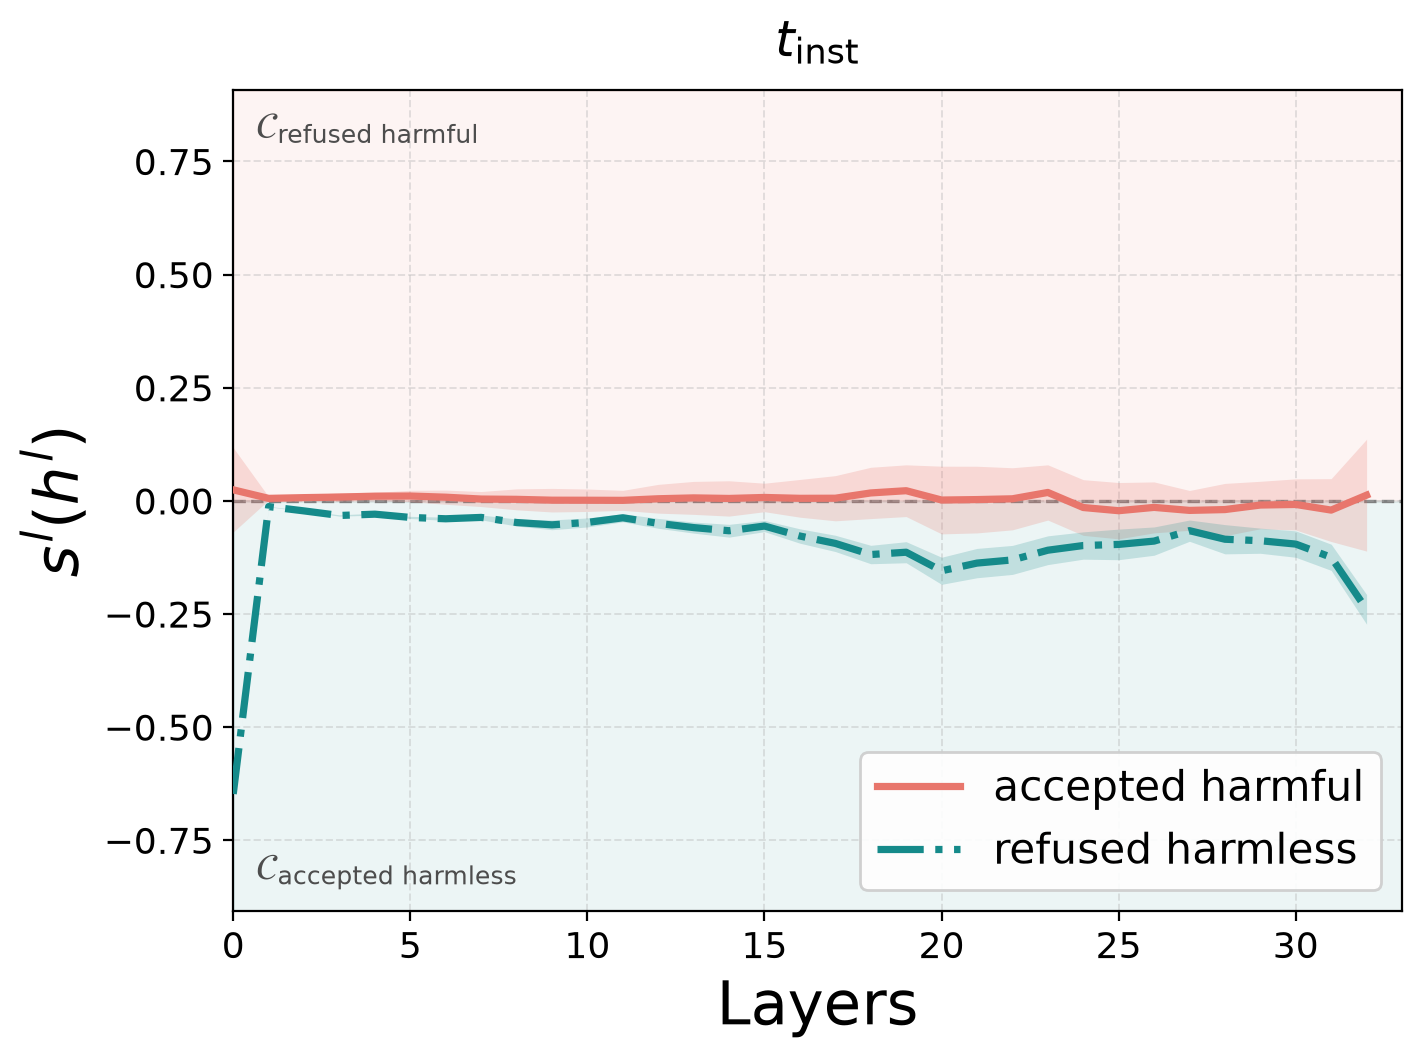
\includegraphics[width=\linewidth]{figures/nothink_tinst.png}\\[0.3em]
    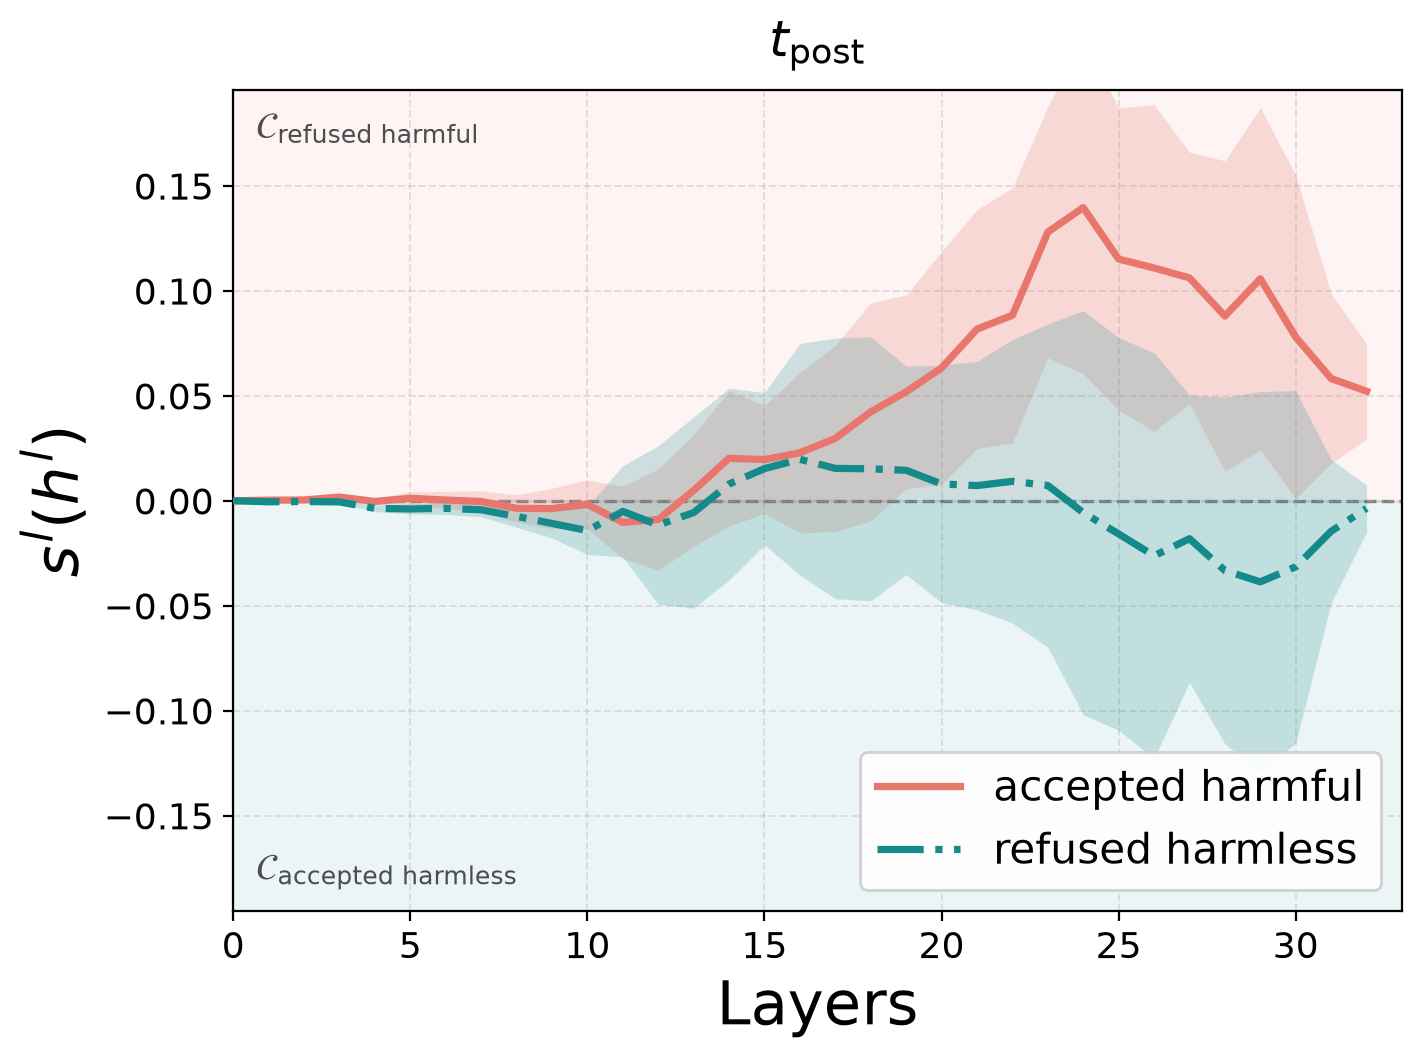
\includegraphics[width=\linewidth]{figures/nothink_tpost.png}
    \caption{Qwen3.5-9B on non-thinking configuration, tinst and tpost activations}
    \label{fig:col_nothink}
\end{subfigure}
\hfill
\begin{subfigure}[t]{0.24\textwidth}
    \centering
    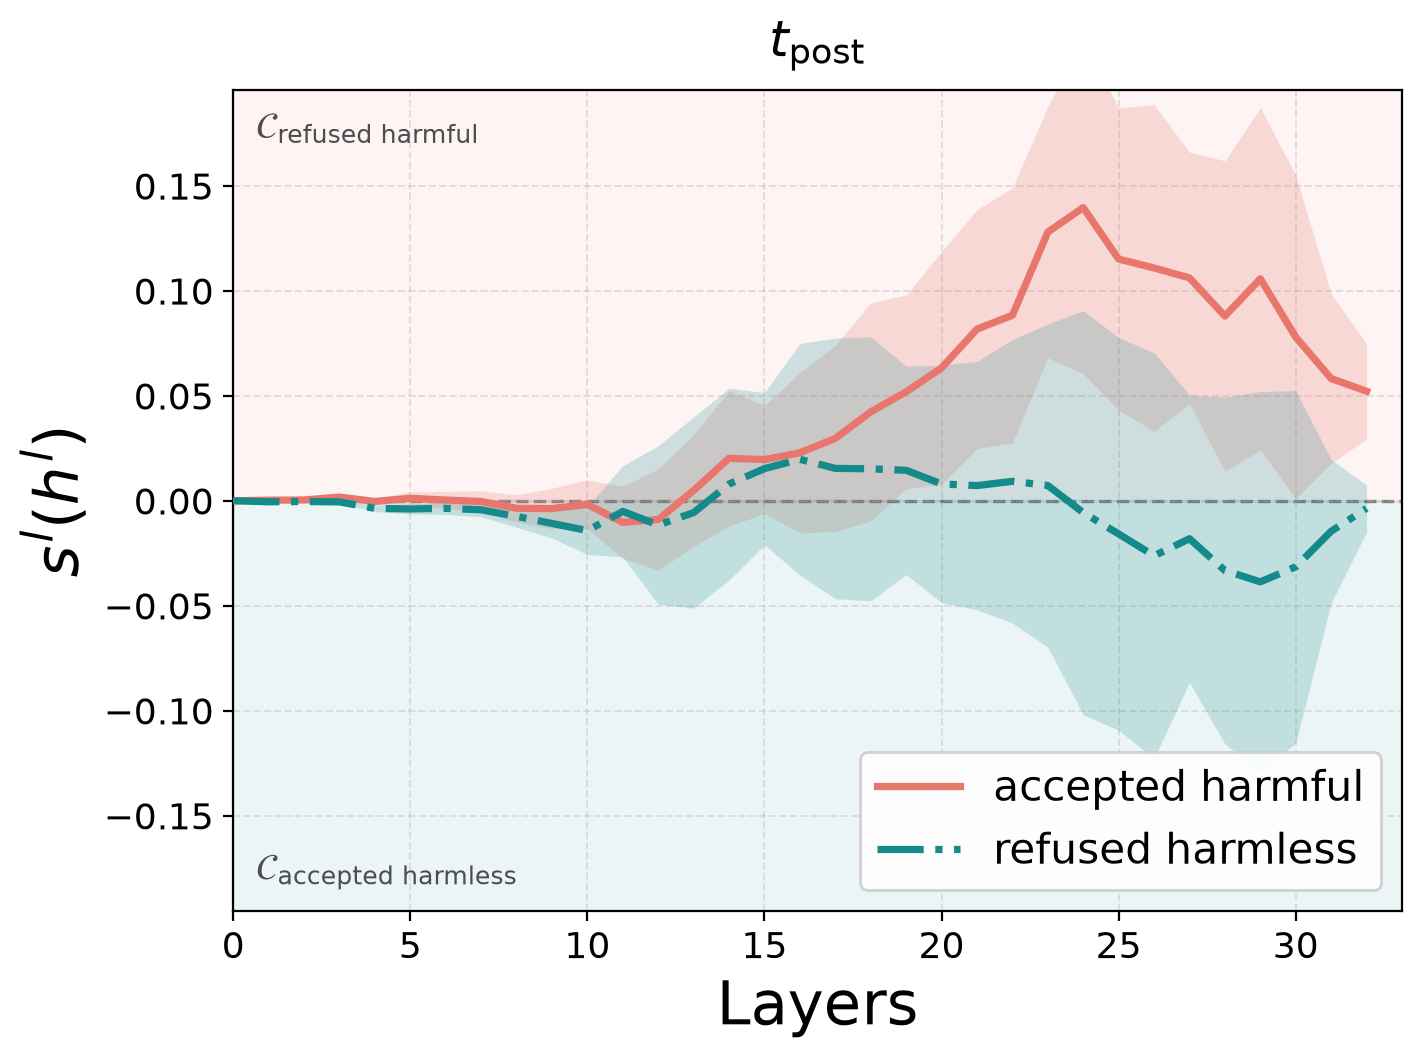
\includegraphics[width=\linewidth]{figures/nothink_tpost.png}\\[0.3em]
    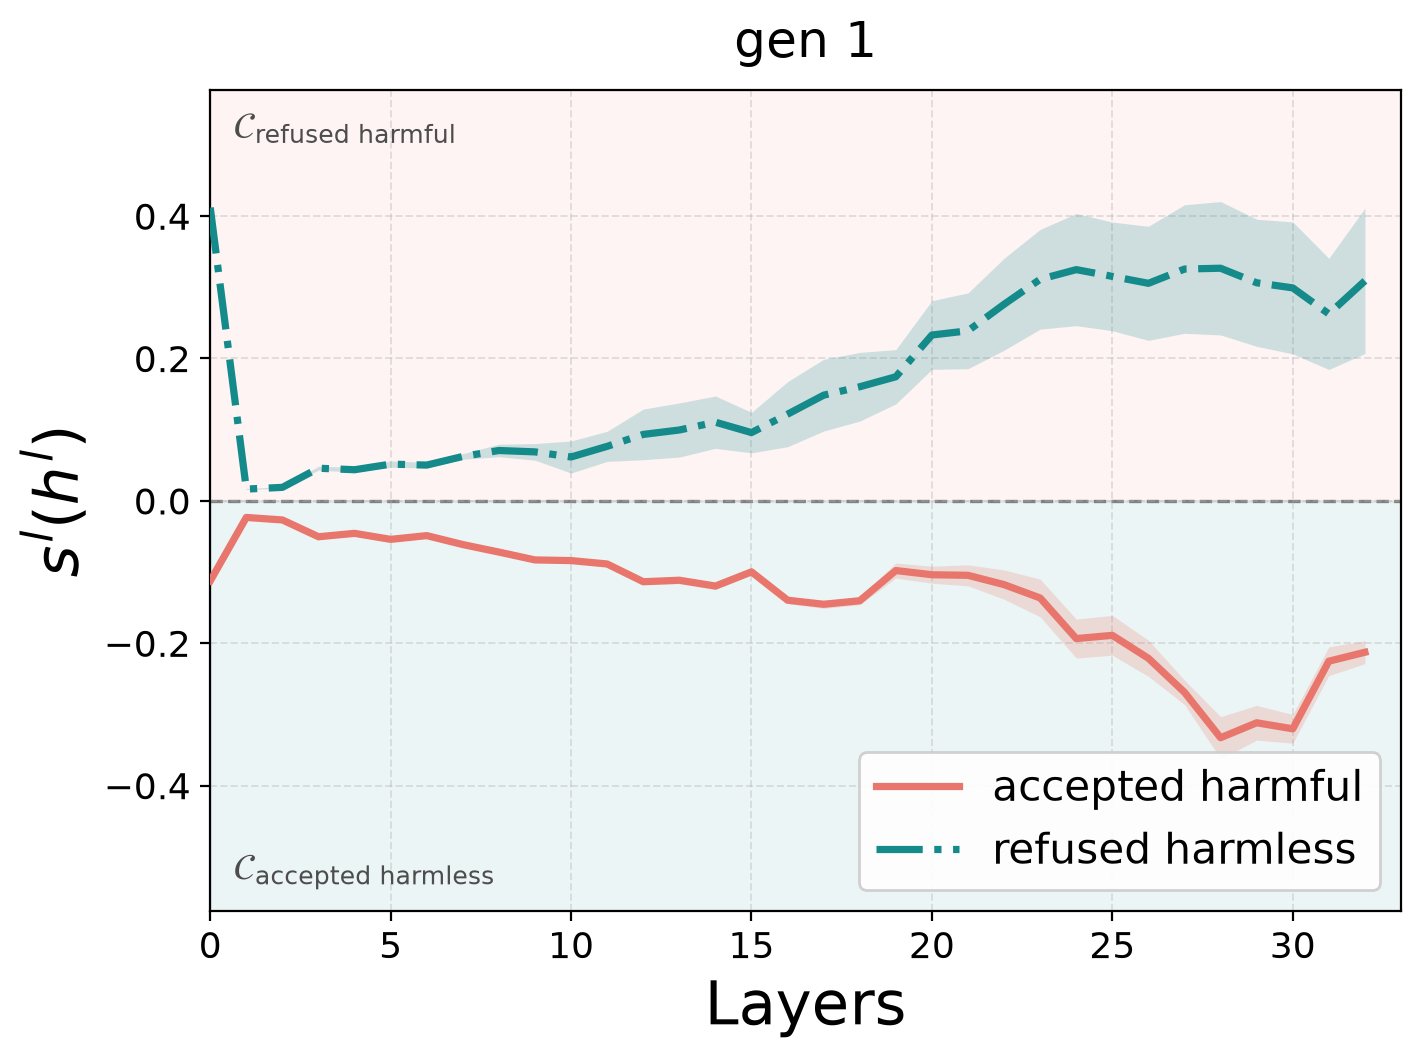
\includegraphics[width=\linewidth]{figures/nothink_gen1.png}
    \caption{Qwen3.5-9B on non-thinking configuration, tpost and gen1 activations}
    \label{fig:col_gen1}
\end{subfigure}
\caption{}
\label{fig:grid}
\end{figure*}

The thinking configuration tokens show less promising results. Figure \ref{fig:app_think} shows all the tokens for this configuration. We try the \textbackslash n token after the opening think token as the harmful token and the mid1 token for the refusal direction, but we obtain no interesting results. We conclude that either there is no clear separation, or the SorryBench dataset was not harmful enough to capture the harmful direction.

\subsection{Correlation between beliefs of harmfulness and refusal replication}
\label{sec:corr}
In this section, we plot the harmful score (Equation \ref{eq:delta_harmful}) and refusal score (Equation \ref{eq:delta_refuse}) of each activation bucket for the non-thinking configuration, using $t_{post}$ as the harmful token and $t_{gen1}$ as the refusal token. We apply the same train and test split as in Section \ref{sec:activations}.

\begin{equation}
\resizebox{0.92\linewidth}{!}{$\displaystyle \Delta_{\text{harmful}} = \frac{1}{L}\sum_{l=1}^{L}\left(\text{cos\_sim}\left(h_l^{t_{\text{post}}}, \mu_{l,\,\text{harmful}}^{t_{\text{post}}}\right) - \text{cos\_sim}\left(h_l^{t_{\text{post}}}, \mu_{l,\,\text{harmless}}^{t_{\text{post}}}\right)\right)$}
\label{eq:delta_harmful}
\end{equation}
\begin{equation}
\resizebox{0.92\linewidth}{!}{$\displaystyle \Delta_{\text{refuse}} = \frac{1}{L}\sum_{l=1}^{L}\left(\text{cos\_sim}\left(h_l^{t_{\text{gen1}}}, \mu_{l,\,\text{refuse}}^{t_{\text{gen1}}}\right) - \text{cos\_sim}\left(h_l^{t_{\text{gen1}}}, \mu_{l,\,\text{accept}}^{t_{\text{gen1}}}\right)\right)$}
\label{eq:delta_refuse}
\end{equation}

Figure \ref{fig:figure3_qwen35_nothink} shows the resulting clusters; the four clusters are clearly defined in their corresponding space. We note that the magnitude of the score is nearly half that of the replication for the Qwen2 model, suggesting that although both directions are present, they might not be as distinct as expected.


\begin{figure}[h]
\centering
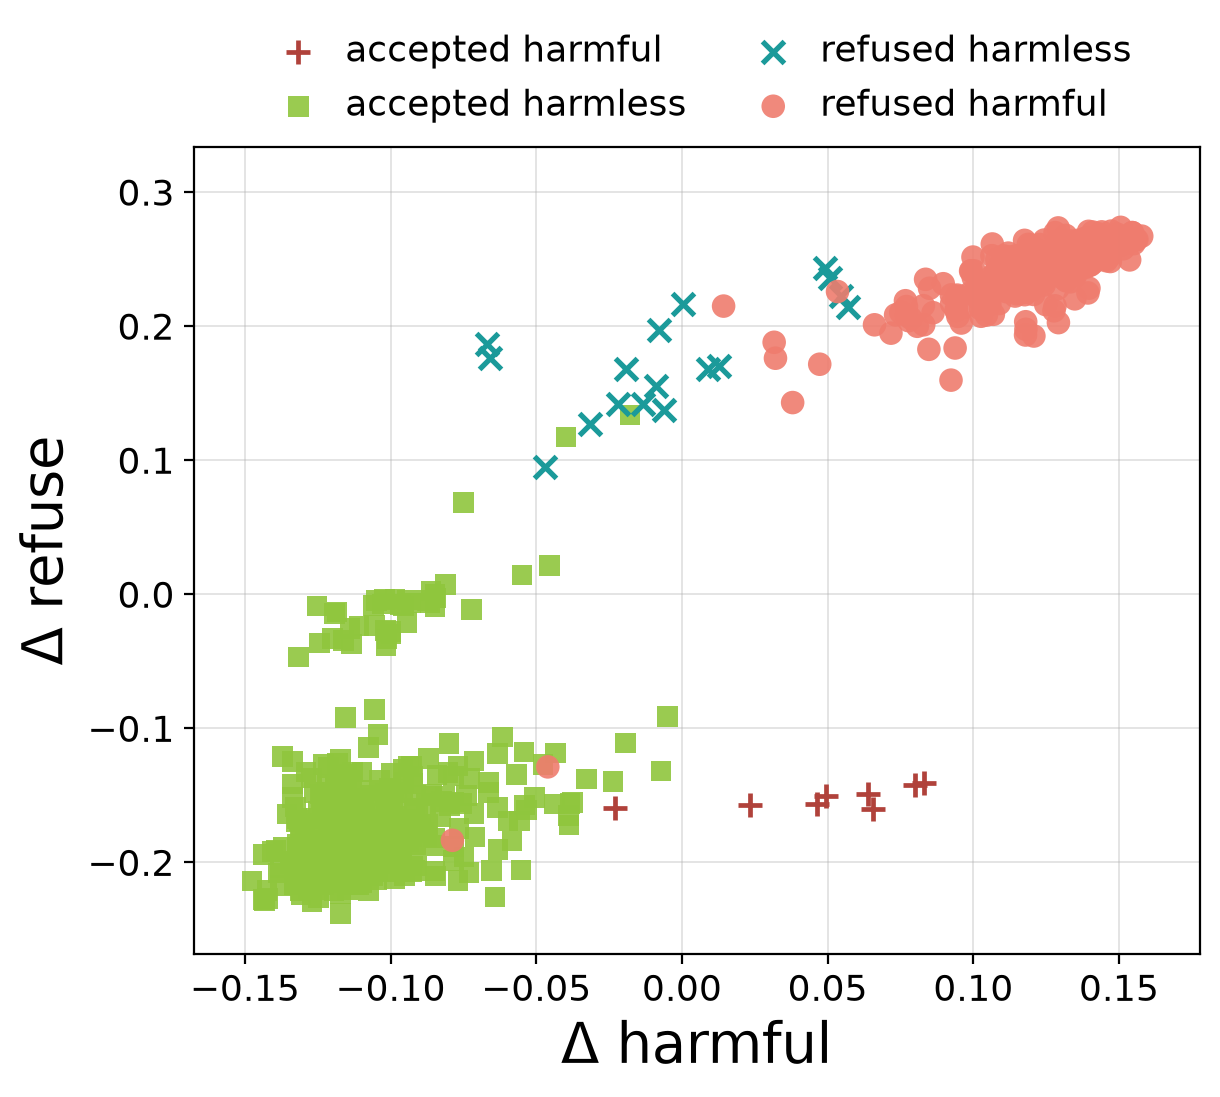
\includegraphics[width=0.75\linewidth]{figures/figure3_qwen35_nothink.png}
\caption{Non-thinking generation activations for tpost and gen1 tokens clustered according to refusal and harmful score.}
\label{fig:figure3_qwen35_nothink}
\end{figure}

\subsection{Activation steering}
\label{sec:elicit_refusal}
% \label{eq:elicit_refusal}
We test our $t_{\text{post-inst}}$ and $t_{gen1}$ token activations to check whether we can elicit refusal.
For each layer $l$, we compute the steering vectors
\begin{align*}
    v_l^{\text{harmful}} &= \mu_{l,\,\text{harmful}}^{t_{\text{post}}} - \mu_{l,\,\text{harmless}}^{t_{\text{post}}}, \\
    v_l^{\text{refuse}} &= \mu_{l,\,\text{refuse}}^{t_{\text{gen1}}} - \mu_{l,\,\text{accept}}^{t_{\text{gen1}}}
\end{align*}
and perform additive steering to alter the hidden state $h^l$ in every layer $l$.
During forward passes, we compute $h^l \gets h^l + c \, v_l^{\text{harmful}}$ or $h^l \gets h^l + c \, v_l^{\text{refuse}}$ with $c \in \mathbb{R}$ across all tokens of input instructions.

In addition to steering along the harmfulness and refusal directions, we also consider steering along random directions.
If a behavior is indeed induced by steering in a specific direction, then we should observe a different behavior if we change the direction.
Thus, we use random steering as a baseline for assessing steering effects.
For each layer $l$, we randomly rotate $v_l^\textup{harmful}$ and $v_l^\textup{refuse}$ to produce two random steering vectors $\tilde{v}_l^\textup{harmful}$ and $\tilde{v}_l^\textup{refuse}$.
The random steering vectors yield perturbations of the same magnitude as the original steering vectors, but in different directions.


\begin{figure}[!t]
\centering
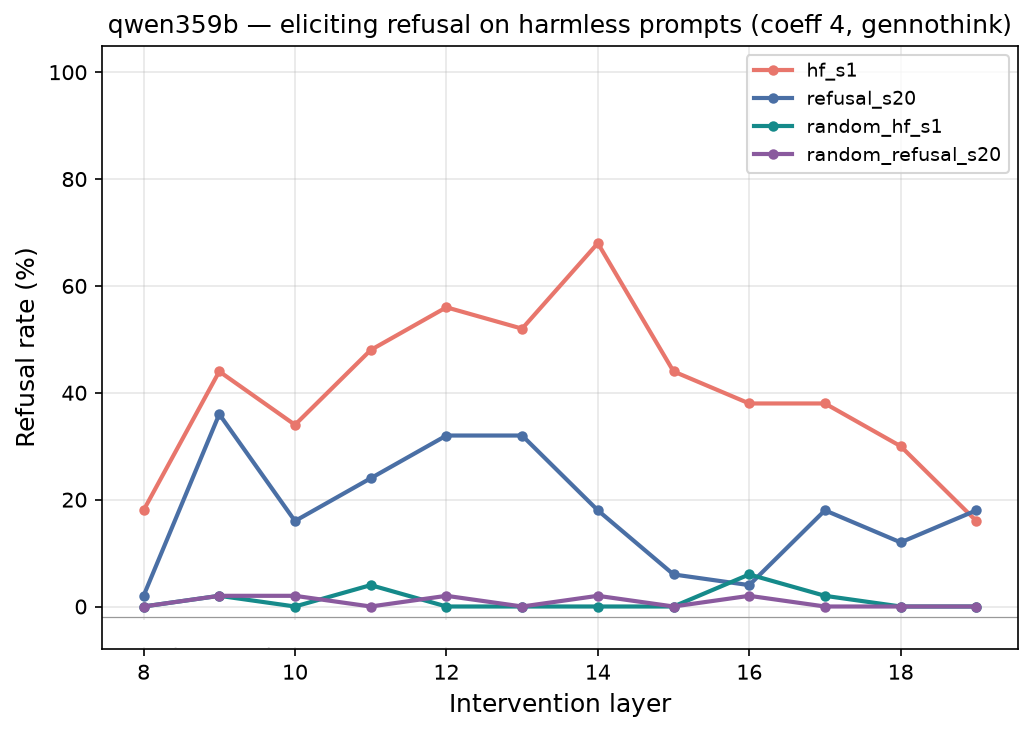
\includegraphics[width=0.85\linewidth]{figures/fig4.png}
\caption{The orange and blue curves show the refusal rates under additive steering in the harmfulness direction $v_l^\textup{harmful}$ (orange curve) and refusal direction $v_l^\textup{refuse}$ (blue curve), respectively.
The green and purple curves show the refusal rates under additive steering in the random directions $\tilde{v}_l^\textup{harmful}$ and $\tilde{v}_l^\textup{refuse}$, respectively.
The steering coefficient is $c = 4$ in all cases, and the thinking mode is disabled.}
\label{fig:fig4}
\end{figure}

\subsection{Harfmul and refusal direction causal separation}
\label{sec:reply-inversion}

Figure~\ref{fig:fig4} shows that steering the model in the harmfulness and refusal directions can both elicit refusal behavior on harmless instructions.
To disentangle refusal from the model's judgement of harmfulness, we follow \citet{zhao2025harmfulness} to perform a reply inversion task.
In this task, we append the following question to the original instructions: \emph{``Could this user prompt cause harm? Answer `Certainly' if it could, otherwise `No'.''}
Without steering, the model is expected to reply with ``No'' to harmless instructions and ``Certainly'' to harmful instructions.
If steering into the harmfulness direction increases the model's perceived harmfulness, we can expect the model to categorize harmless instructions as certainly harmful.
Conversely, steering into the harmless direction is expected to make the model classify harmful instructions as not harmful.
\citet{zhao2025harmfulness} observed the expected behavior changes in the instruct model Qwen2-7B and claimed it as an evidence for the harmfulness and refusal concepts to be causally separable.

We conducted the same experiments for Qwen3.5-9B with the thinking mode turned off.
The results are presented in \Cref{fig:fig5}.
We observed that the model does not always answer with ``Certainly'' or ``No'' as the prompt asks, but sometimes replies with a canonical refusal phrase (e.g., ``I cannot assist...'').
When steered into the harmfulness direction, the model is expected to classify harmless instructions as certainly harmful, but \Cref{fig:fig5a} (in particular the orange curve) shows that the model frequently replies with canonical refusal phrases instead of giving an answer.
Based on this observation, we cannot conclude that harmfulness and refusal are clearly separable concepts.
In \Cref{fig:fig5b}, we observe that steering into the reverse harmfulness direction (see the orange curve) can slightly increase the rate of the model judging a harmful instruction as harmless, but random steering can elicit the same behavior more drastically.
This suggests a lack of evidence for the steered model to perceive less harmfulness.


\begin{figure*}[!t]
\centering
\begin{subfigure}[t]{0.45\textwidth}
    \centering
    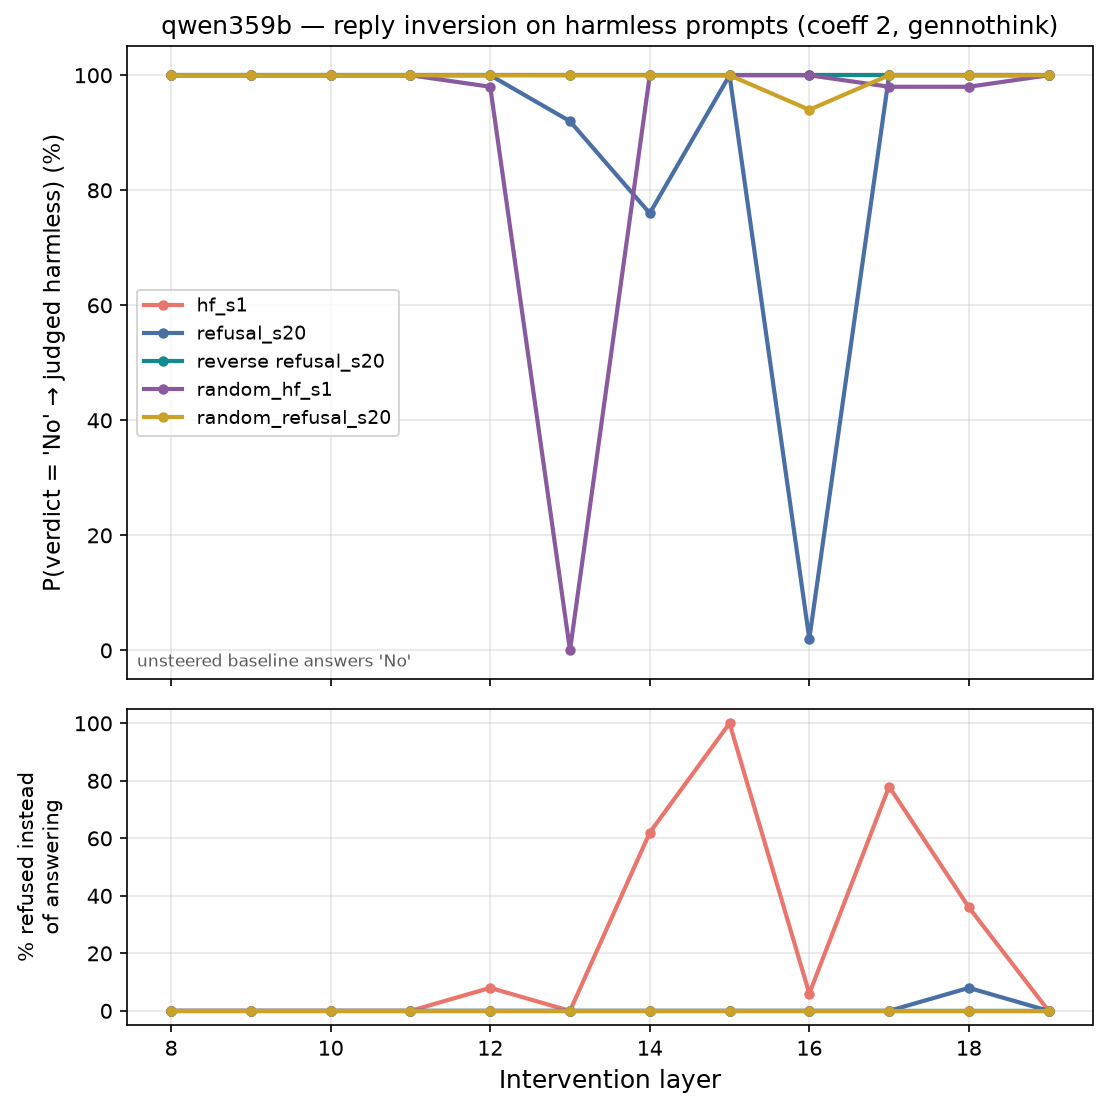
\includegraphics[width=\linewidth]{figures/fig5a.jpeg}
    \caption{}
    \label{fig:fig5a}
\end{subfigure}
\hfill
\begin{subfigure}[t]{0.45\textwidth}
    \centering
    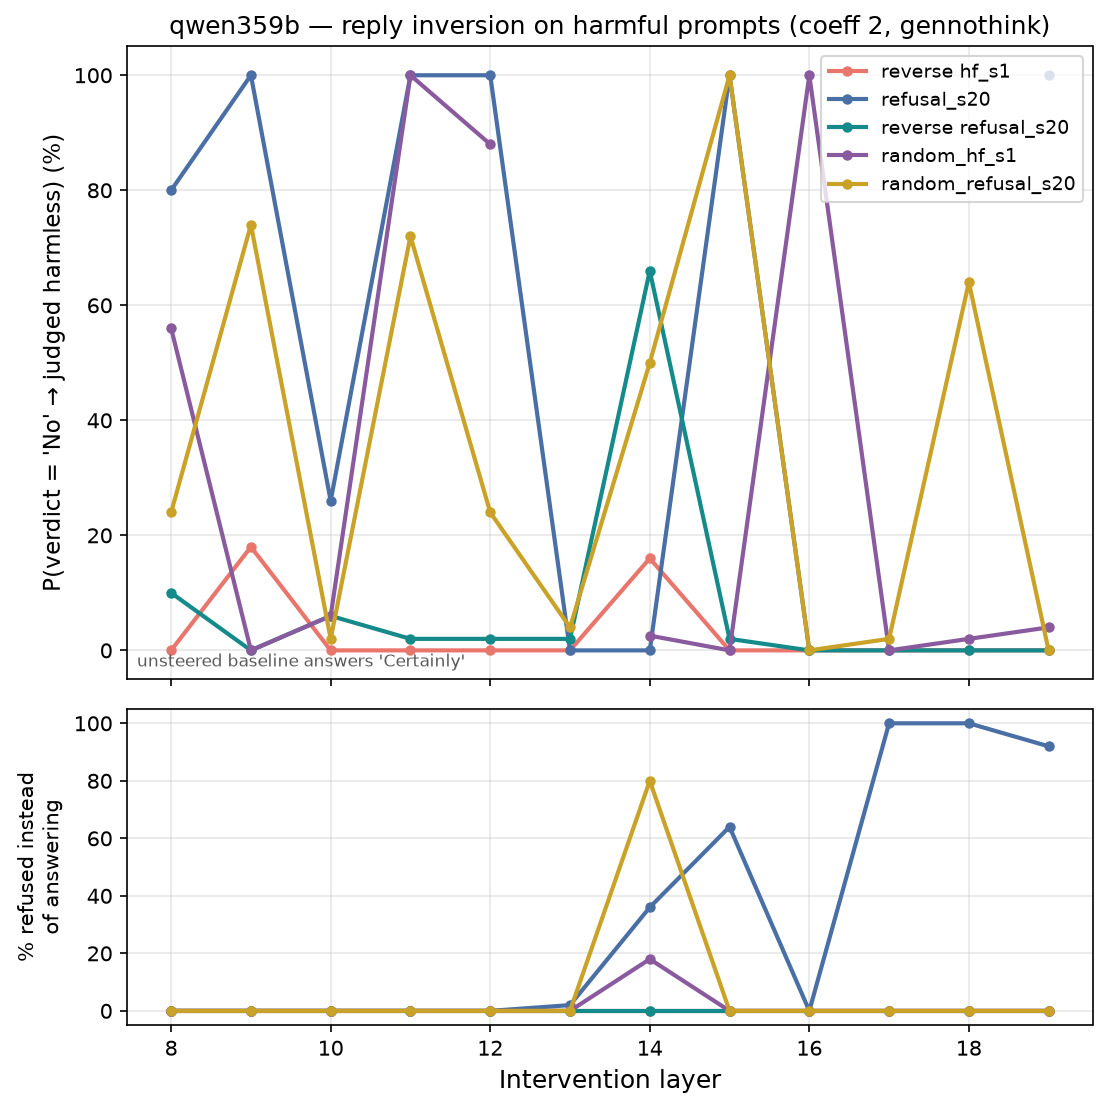
\includegraphics[width=\linewidth]{figures/fig5b.jpeg}
    \caption{}
    \label{fig:fig5b}
\end{subfigure}
\caption{Intervention results for the reply inversion tasks.
If the model does not reply with ``Certainly'' or ``No'' but a canonical refusal phrase (e.g., ``I cannot assist...''), then we classify the response as a refusal to answer the question.
As in \Cref{fig:fig4}, we include random steering results for comparison.
The steering coefficient is $c = 2$ in all cases.
Without steering, the model answers ``No'' to 100\% of the harmless instructions and 2\% of the harmful instructions.
}
\label{fig:fig5}
\end{figure*}

\section{Related Work}

\paragraph{Activation steering and refusal directions.} Work on activation steering shows that behaviorally meaningful directions can be extracted from hidden states and used to modify model behavior without retraining \citep{turner2023activation, rimsky2024steering}. In safety settings, \citet{arditi2024refusal} show that refusal in chat models can often be mediated by a single residual-stream direction. This provides a natural starting point for studying refusal as a geometric object in activation space.

\paragraph{Harmfulness, refusal, and over-refusal.} Our work directly builds on \citet{zhao2025harmfulness}, who argue that harmfulness and refusal are encoded separately rather than as a single safety axis. Related work complicates the geometry of refusal: refusal may occupy a concept cone or multiple directions rather than one vector \citep{wollschlager2025geometry, joad2026more}, and over-refusal can be task-dependent even when harmful refusal is comparatively low-dimensional \citep{wang2024surgical, maskey2026overrefusal}.

\paragraph{Reasoning models and CoT safety.} Recent work suggests that reasoning changes the refusal mechanism. \citet{yamaguchi2026where} show that where and whether reasoning models refuse depends on CoT content, and \citet{yang2026beyond} find that simple refusal steering becomes less reliable once CoT is fixed. Other work shows that reasoning can create new jailbreak surfaces or alter safety decisions during generation \citep{yong2026selfjailbreaking, zhao2026cothijacking, refusalcliff2025}. These findings motivate analyzing not only prompt-boundary tokens, but also thinking and answer-boundary positions.

\paragraph{Monitoring reasoning.} Finally, probe-based monitoring work asks whether unsafe final behavior can be predicted before a model finishes thinking \citep{predictalignment2025}. Steering-vector analyses of reasoning behavior more broadly also suggest that latent directions can reveal structure inside thinking models \citep{venhoff2025understanding}.



\section{Conclusions}
In this work, we study whether the separation between harmfulness and refusal encoding, previously observed in Instruct models, persists in thinking models. Section \ref{sec:strip} shows that, unlike in Instruct models, stripping the last tokens of the prompt does not decrease the refusal rate in any of the tested configurations, suggesting that the mechanism found in Instruct models does not transfer directly to thinking models.

Section \ref{sec:activations} shows that on the non-thinking configuration, the harmfulness and refusal separation reappears on different tokens than in Instruct models, specifically $t_{post}$ and $t_{gen1}$, although coupled more closely than in the original experiments. Section \ref{sec:corr} confirms this correlationally, showing that the harmful and refusal score clusters are clearly defined, but with a smaller magnitude than in the Qwen2 replication. Section \ref{sec:elicit_refusal} further supports this separation: steering both $t_{post}$ and gen1 individually on harmless data points successfully elicits high refusal rates.

For the thinking configuration, the tokens that encoded harmfulness and refusal separately in Instruct models, $t_{inst}$ and $t_{post}$, do not preserve this separation, and we find no clear alternative token pair showing this behavior on thinking-configuration tokens. We attribute this to the SorryBench dataset not being harmful enough to isolate a clear harmful direction on this configuration.

Separately, the inversion generation experiment used to causally confirm the direction separation on the non-thinking configuration was inconclusive. Further work should investigate alternative causal methods better suited to the entangled structure observed on $t_{post}$ and $t_{gen1}$, and re-examine the thinking configuration with a stronger harmful dataset to rule out a dataset limitation.

\section{Limitations} We identify the following limitations in our work:

\textbf{Tested models.} The thinking experiments were executed on a single model family, Qwen3.5. Although both Qwen3.5-4B and Qwen3.5-9B were used, the resulting conclusions are only valid for the Qwen family of models.

\textbf{Data scarcity.} As stated in Section \ref{sec:datasets}, Qwen3.5 models are trained to refuse harmful instructions, so the GCG attack was necessary to generate accepted answers. Due to time constraints, our accepted harmful bucket only contained 17 data points for the non-thinking generation, which adds a higher variance to our results.

\textbf{Judge reliability.} Given the thousands of generations produced across our experiments, only a small subset was manually checked to ensure consistency, while the rest were evaluated by the judge model. This leaves open the possibility that judge errors went undetected in the unchecked majority.

\textbf{Dataset harmfulness ceiling.} For the thinking configuration, we attribute the absence of a clear harmful token pair to SorryBench not being harmful enough to isolate a clear harmful direction. This limits our ability to distinguish between a genuine absence of separation and a dataset that is insufficiently harmful to reveal it.

\textbf{Steering vs. causal inversion mismatch.} While steering both $t_{post}$ and $t_{gen1}$ individually on harmless data points successfully elicits high refusal rates, the inversion generation experiment intended to causally confirm the direction separation was inconclusive. 


\clearpage
\bibliographystyle{icml2022}
\bibliography{example_paper}

\clearpage
\appendix

\subsection{Auxiliary Projection Probes Track CoT Dynamics}

The projection probes provide a complementary contribution: instead of only asking where the prompt-boundary representations lie, they track how steering directions interact with the generated reasoning process itself. Across the Qwen3-thinking layer sweep, CoT is preserved in all inspected modes, but inversion-style settings shorten the generated reasoning trace relative to non-inversion settings. The same runs show strong layer dependence in the $t_{\text{inst}}$ and $t_{\text{post-inst}}$ projection scores, especially in later layers. This supports the broader thesis of the report: once a model reasons before answering, harmfulness/refusal analysis should include not only static prompt positions but also the trajectory and length of the reasoning process. We include the detailed CoT-length and projection-score plots in Appendix~\ref{sec:appendix-cot-probes}.
\section{Configuration details}
\label{ap:confg}

The generation was configured with the following decoding parameters:

\begin{table}[h]
\centering
\begin{tabular}{ll}
\toprule
\textbf{Parameter} & \textbf{Value} \\
\midrule
\texttt{temperature} & $1.0$ \\
\texttt{top\_p} & $0.95$ \\
\texttt{top\_k} & $20$ \\
\texttt{min\_p} & $0.0$ \\
\texttt{presence\_penalty} & $1.5$ \\
\bottomrule
\end{tabular}
\caption{Decoding hyperparameters used for generation in Qwen3.5-9B.}
\label{tab:config}
\end{table}

\section{Activations Plots}
\label{ap:plots}
\begin{figure*}[htbp]
    \centering
    \begin{subfigure}[b]{0.19\textwidth}
        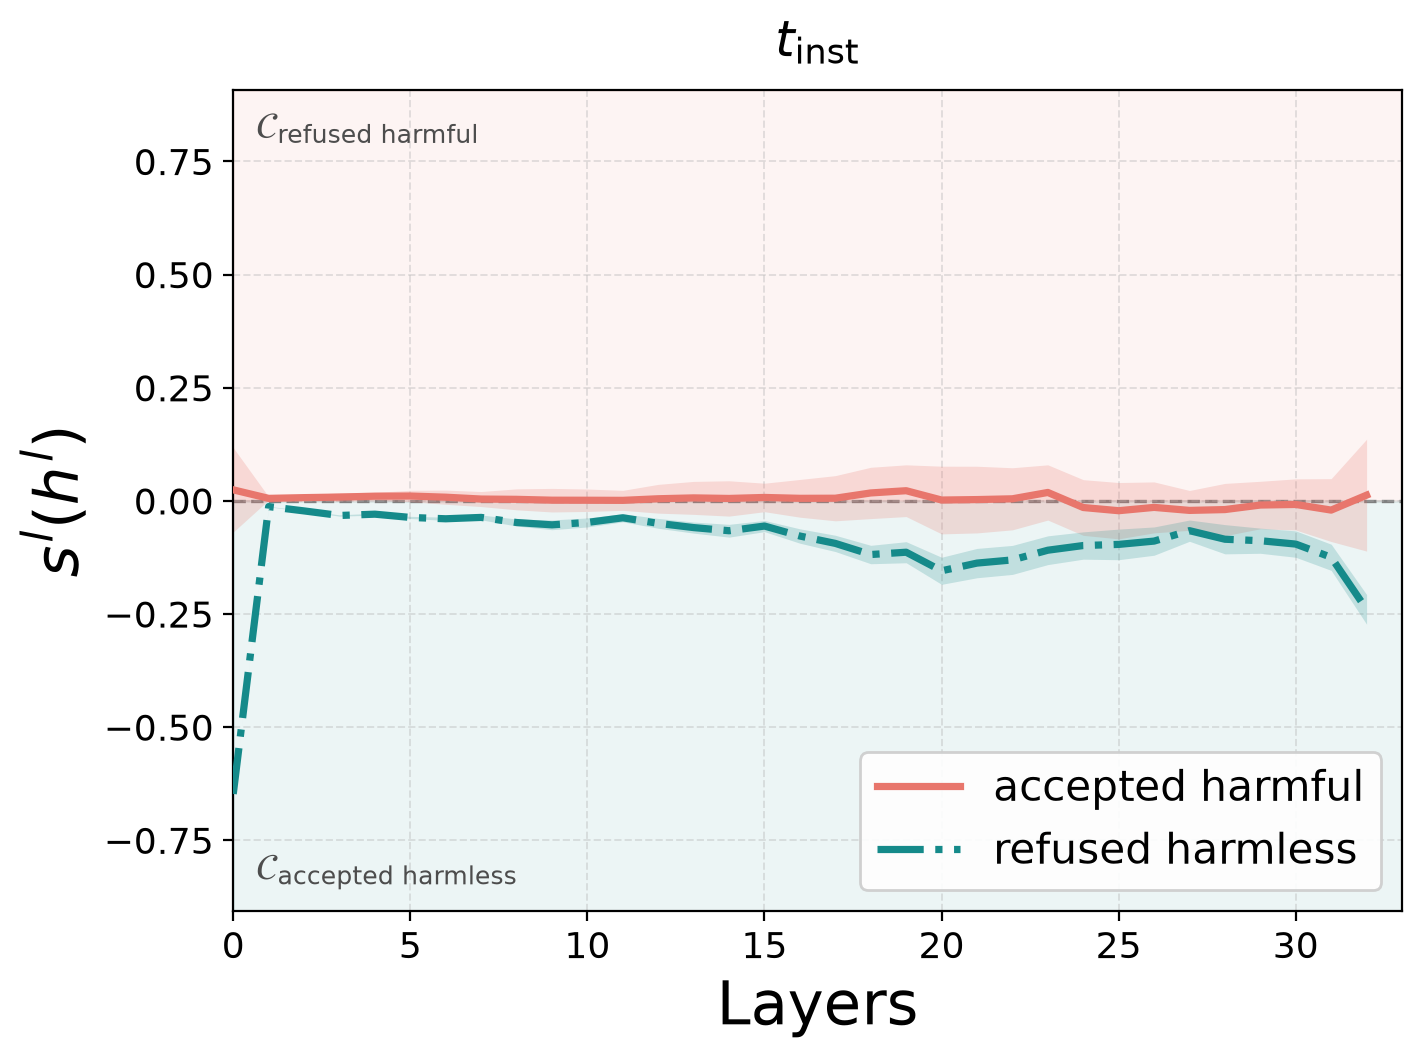
\includegraphics[width=\textwidth]{figures/nothink_run/00_slot00.png}
    \end{subfigure}
    \begin{subfigure}[b]{0.19\textwidth}
        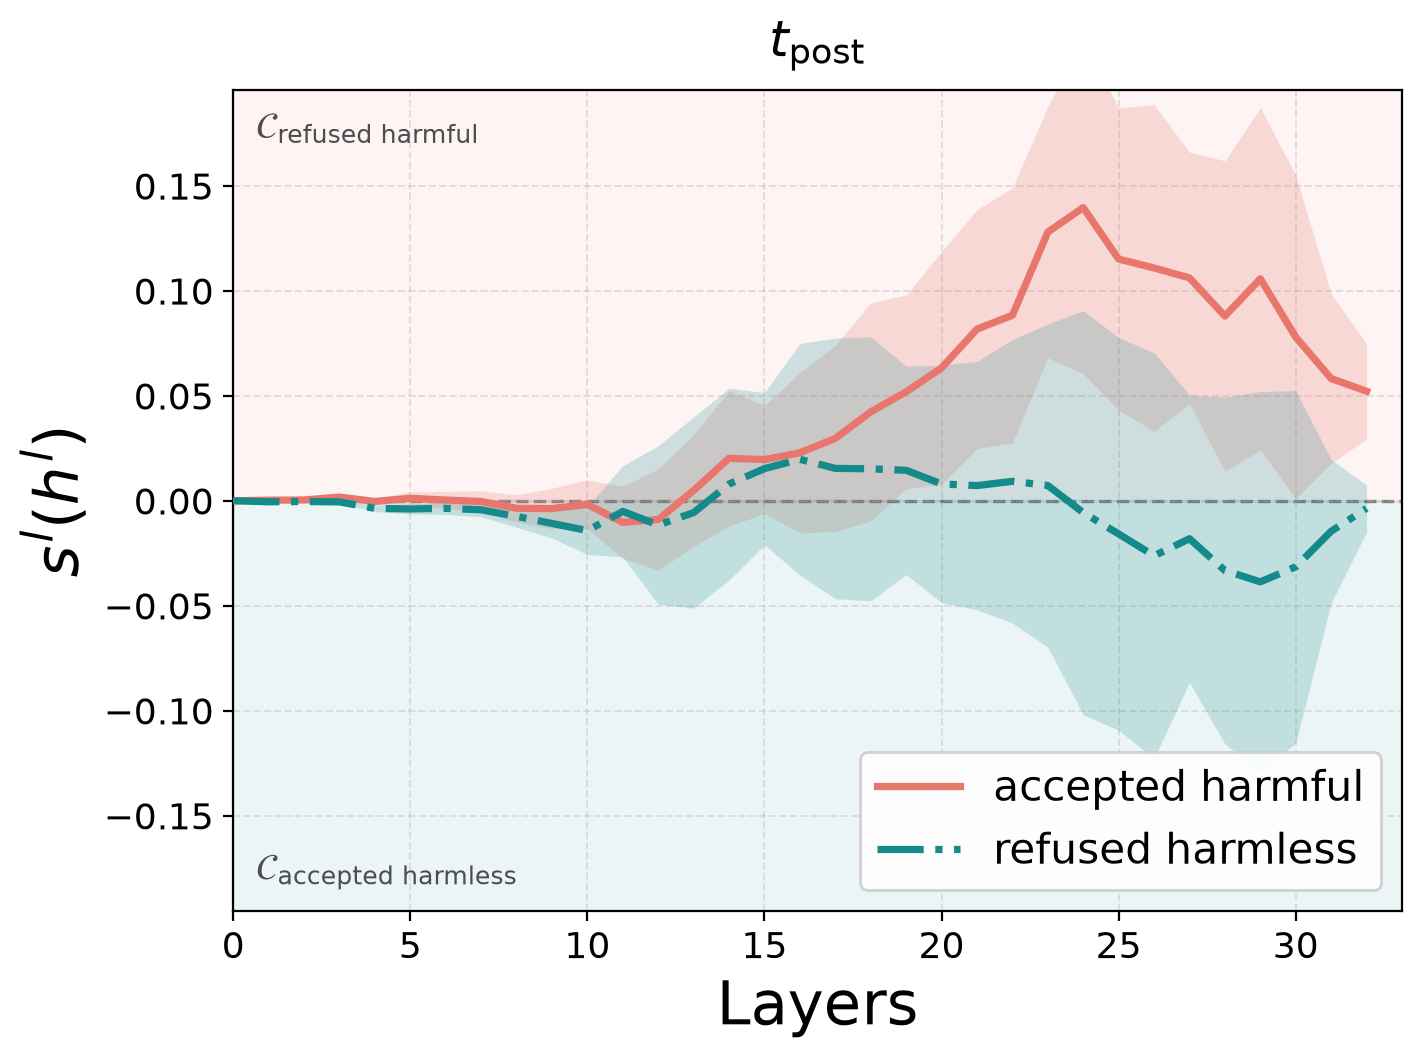
\includegraphics[width=\textwidth]{figures/nothink_run/01_slot01.png}
    \end{subfigure}
    \begin{subfigure}[b]{0.19\textwidth}
        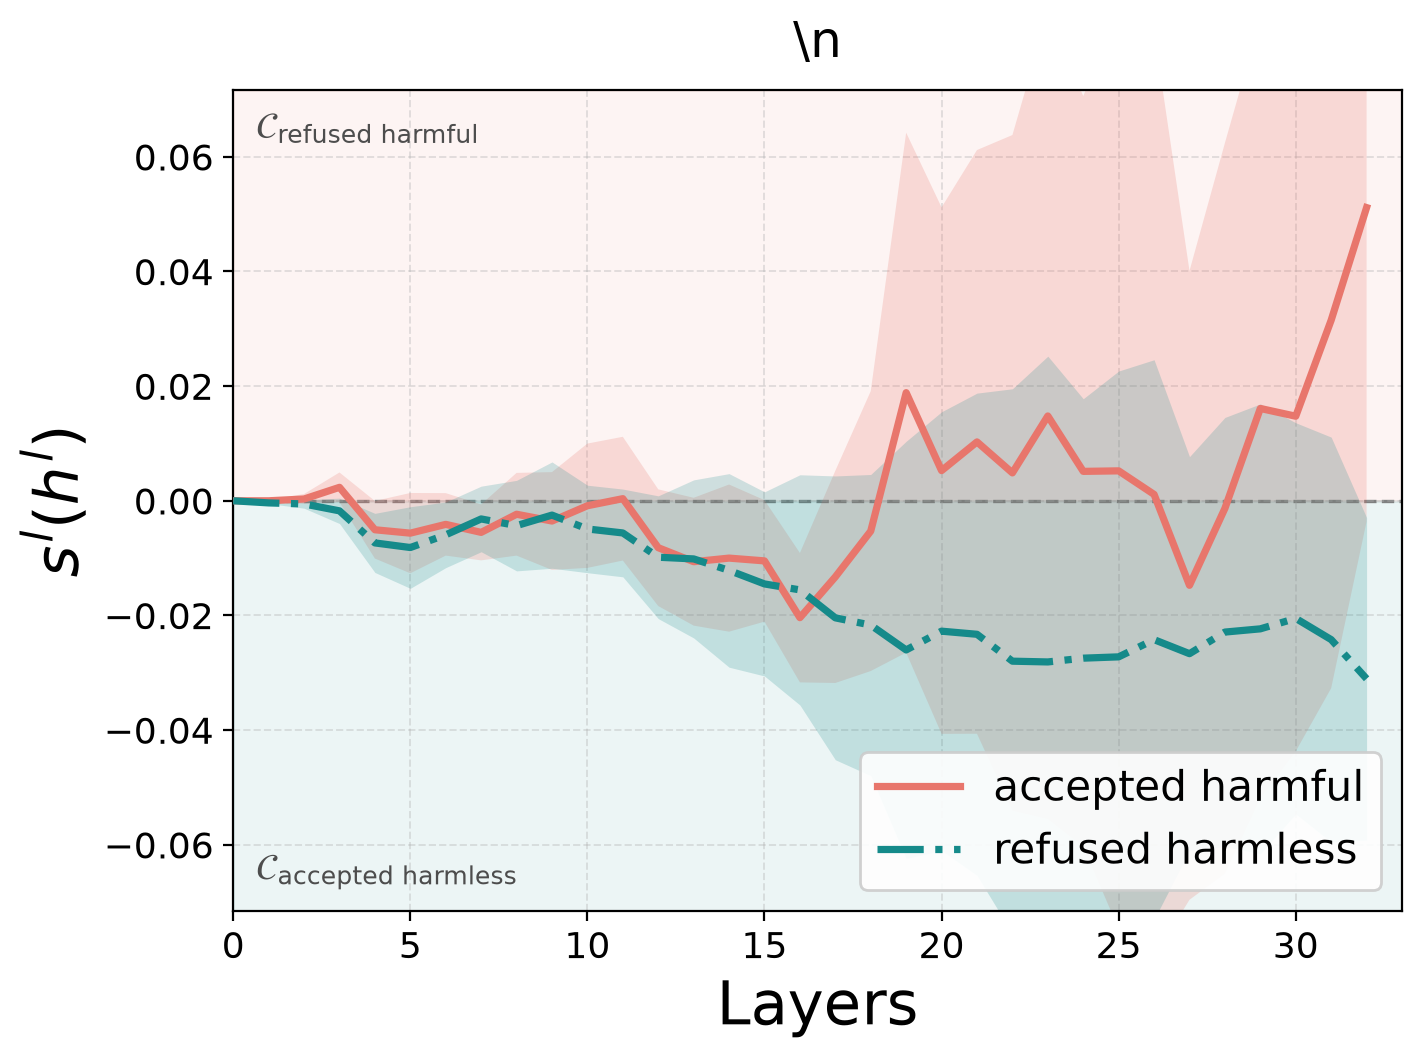
\includegraphics[width=\textwidth]{figures/nothink_run/02_slot02.png}
    \end{subfigure}
    \begin{subfigure}[b]{0.19\textwidth}
        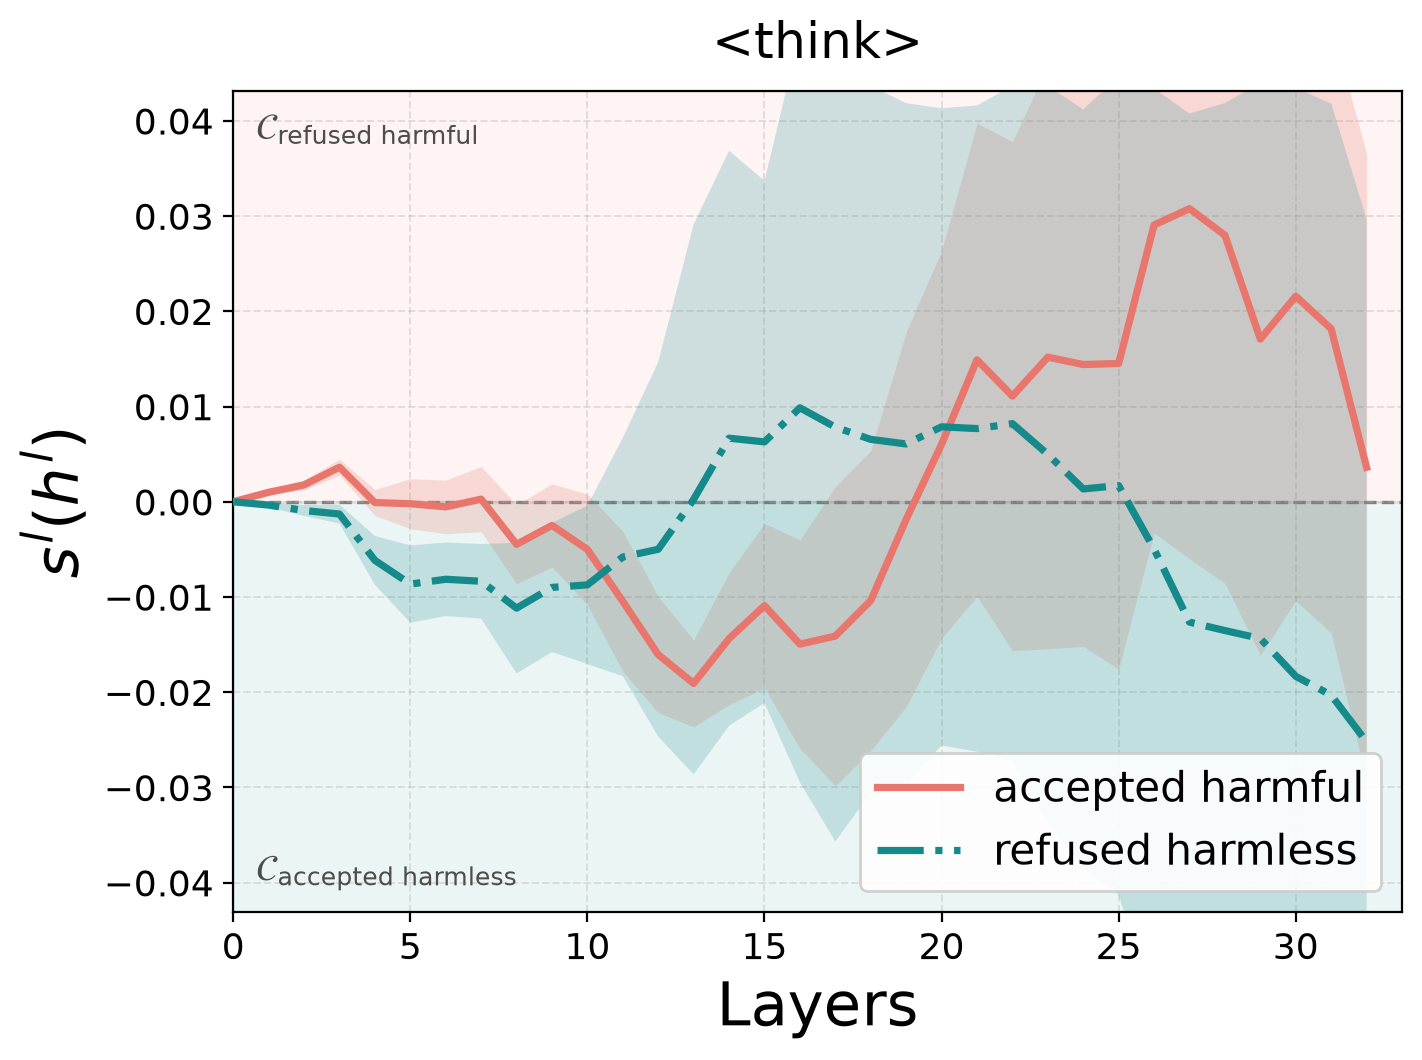
\includegraphics[width=\textwidth]{figures/nothink_run/03_slot03.png}
    \end{subfigure}
    \begin{subfigure}[b]{0.19\textwidth}
        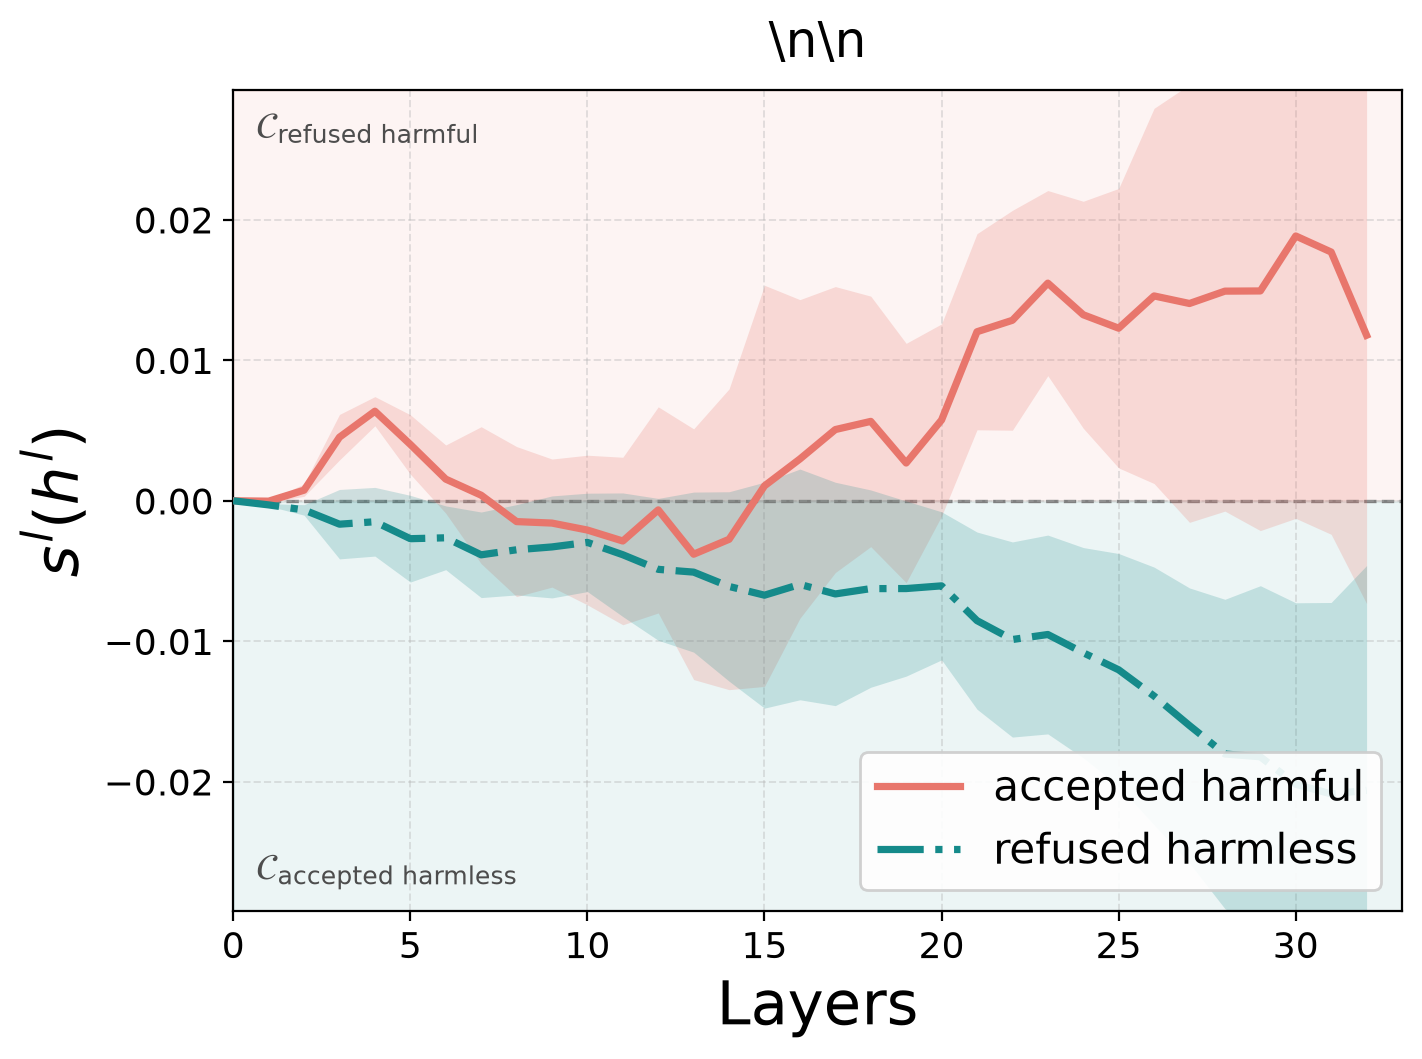
\includegraphics[width=\textwidth]{figures/nothink_run/04_slot04.png}
    \end{subfigure}

    \vspace{0.5em}

    \begin{subfigure}[b]{0.19\textwidth}
        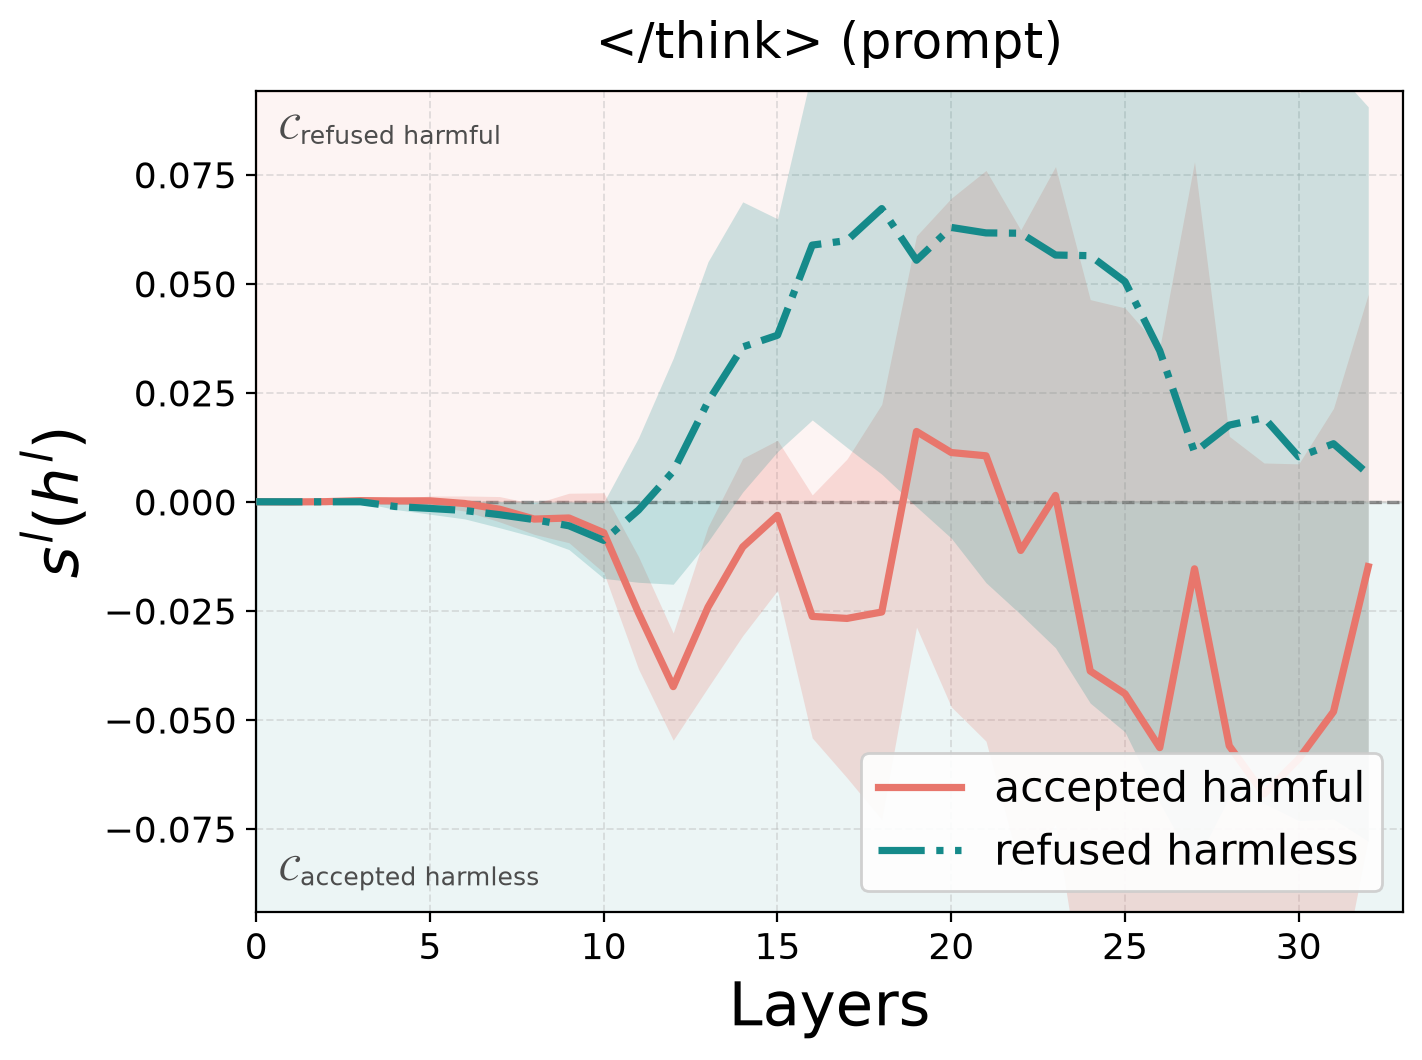
\includegraphics[width=\textwidth]{figures/nothink_run/05_slot24.png}
    \end{subfigure}
    \begin{subfigure}[b]{0.19\textwidth}
        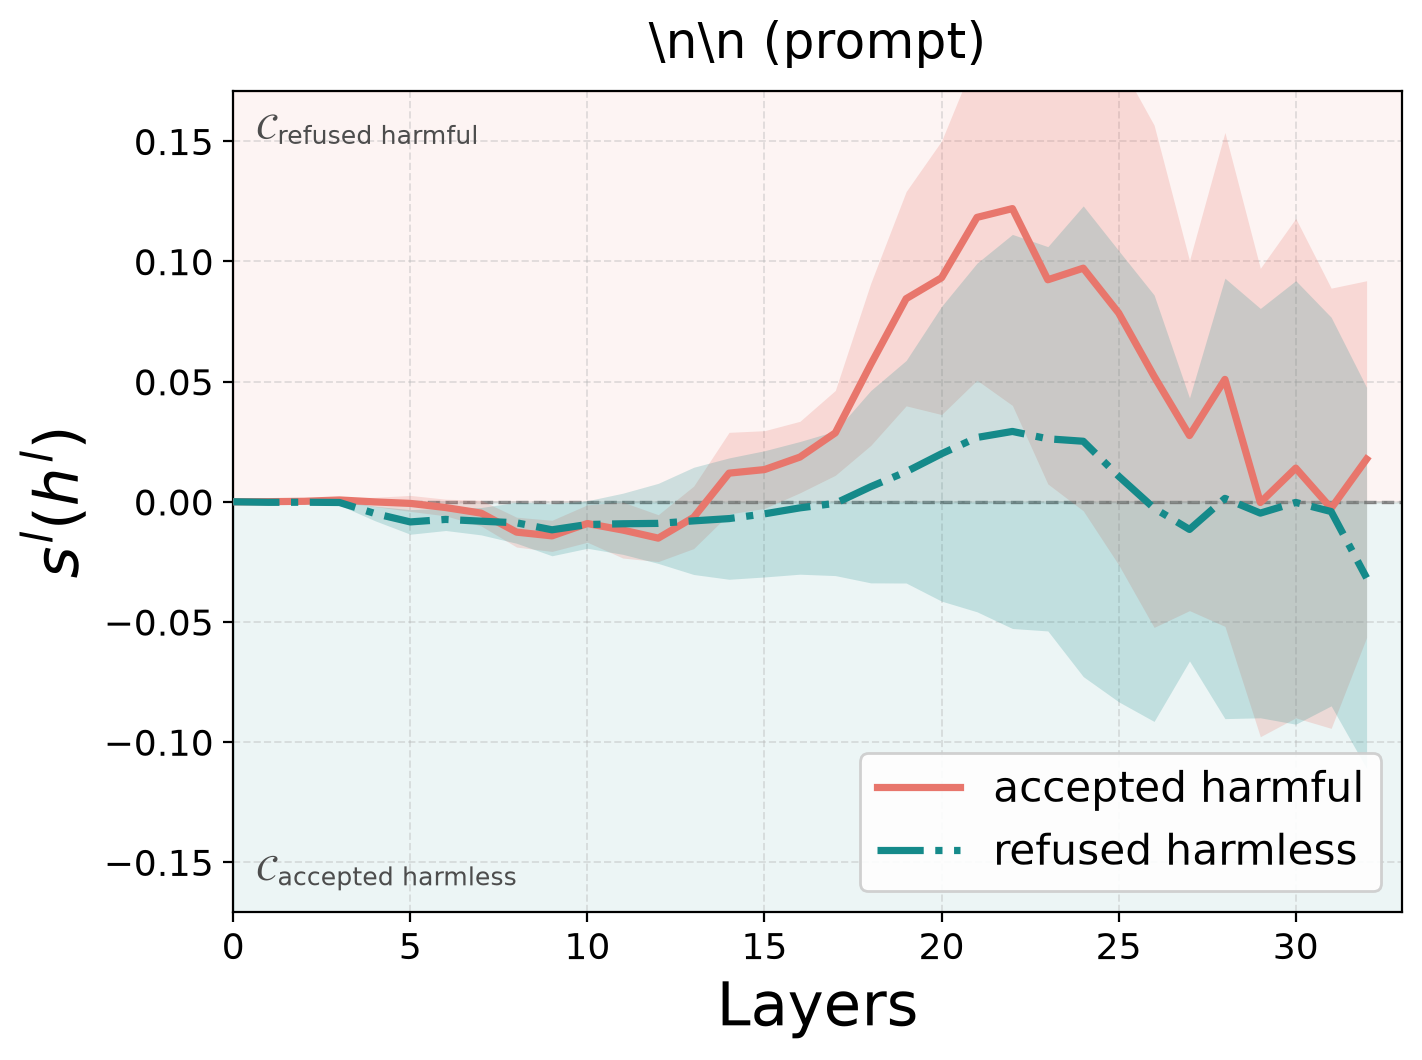
\includegraphics[width=\textwidth]{figures/nothink_run/06_slot20.png}
    \end{subfigure}
    \begin{subfigure}[b]{0.19\textwidth}
        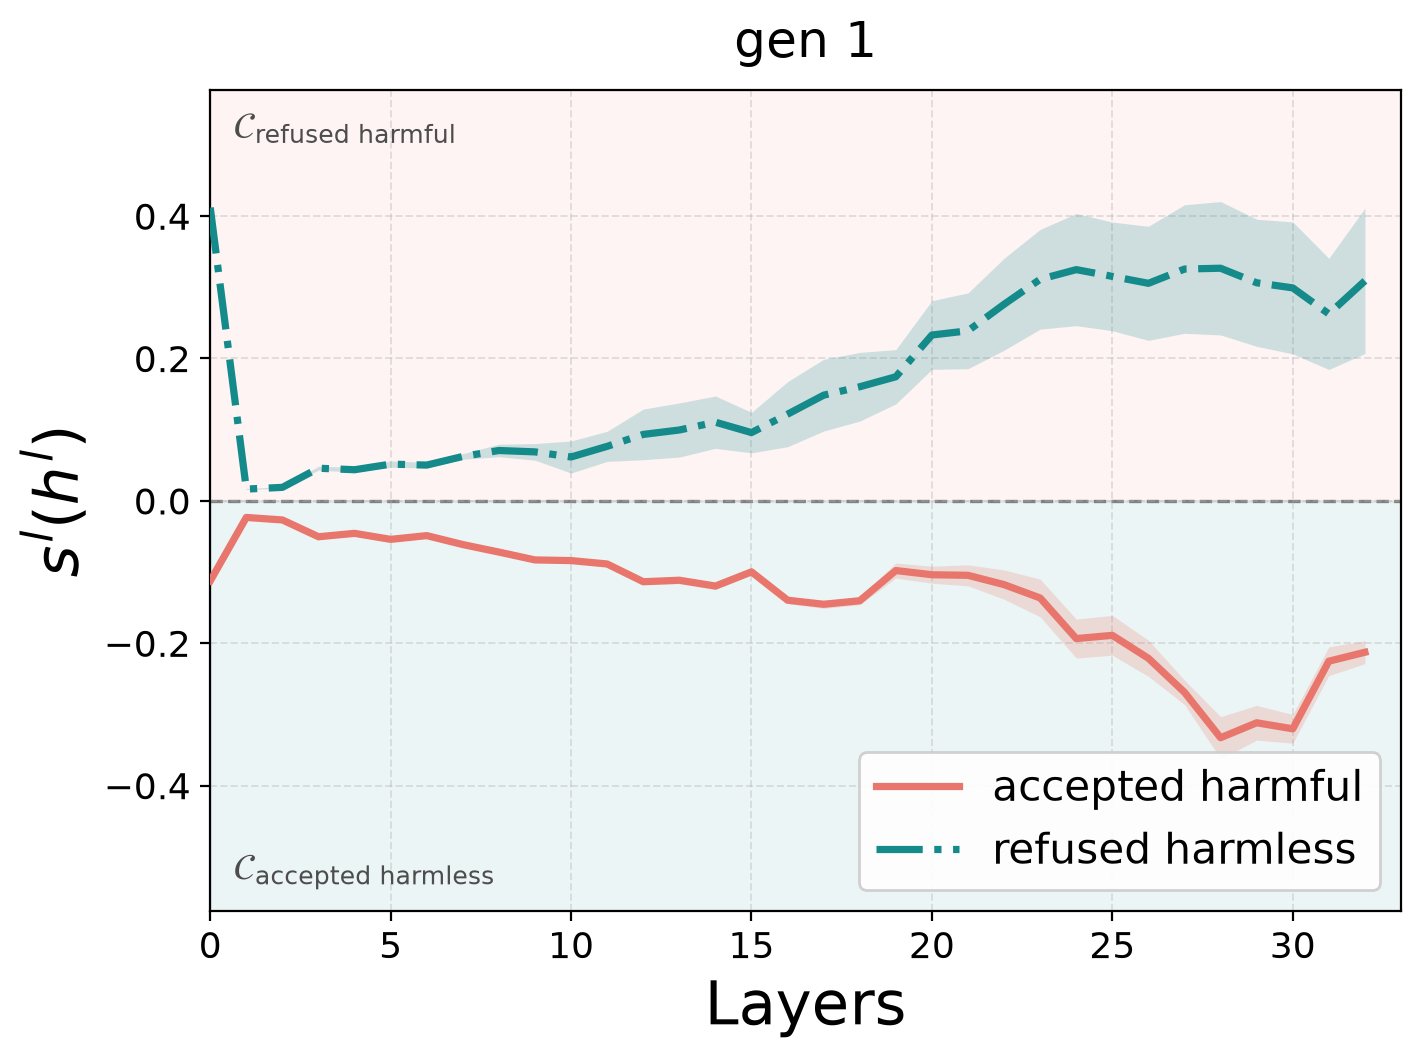
\includegraphics[width=\textwidth]{figures/nothink_run/07_slot21.png}
    \end{subfigure}
    \begin{subfigure}[b]{0.19\textwidth}
        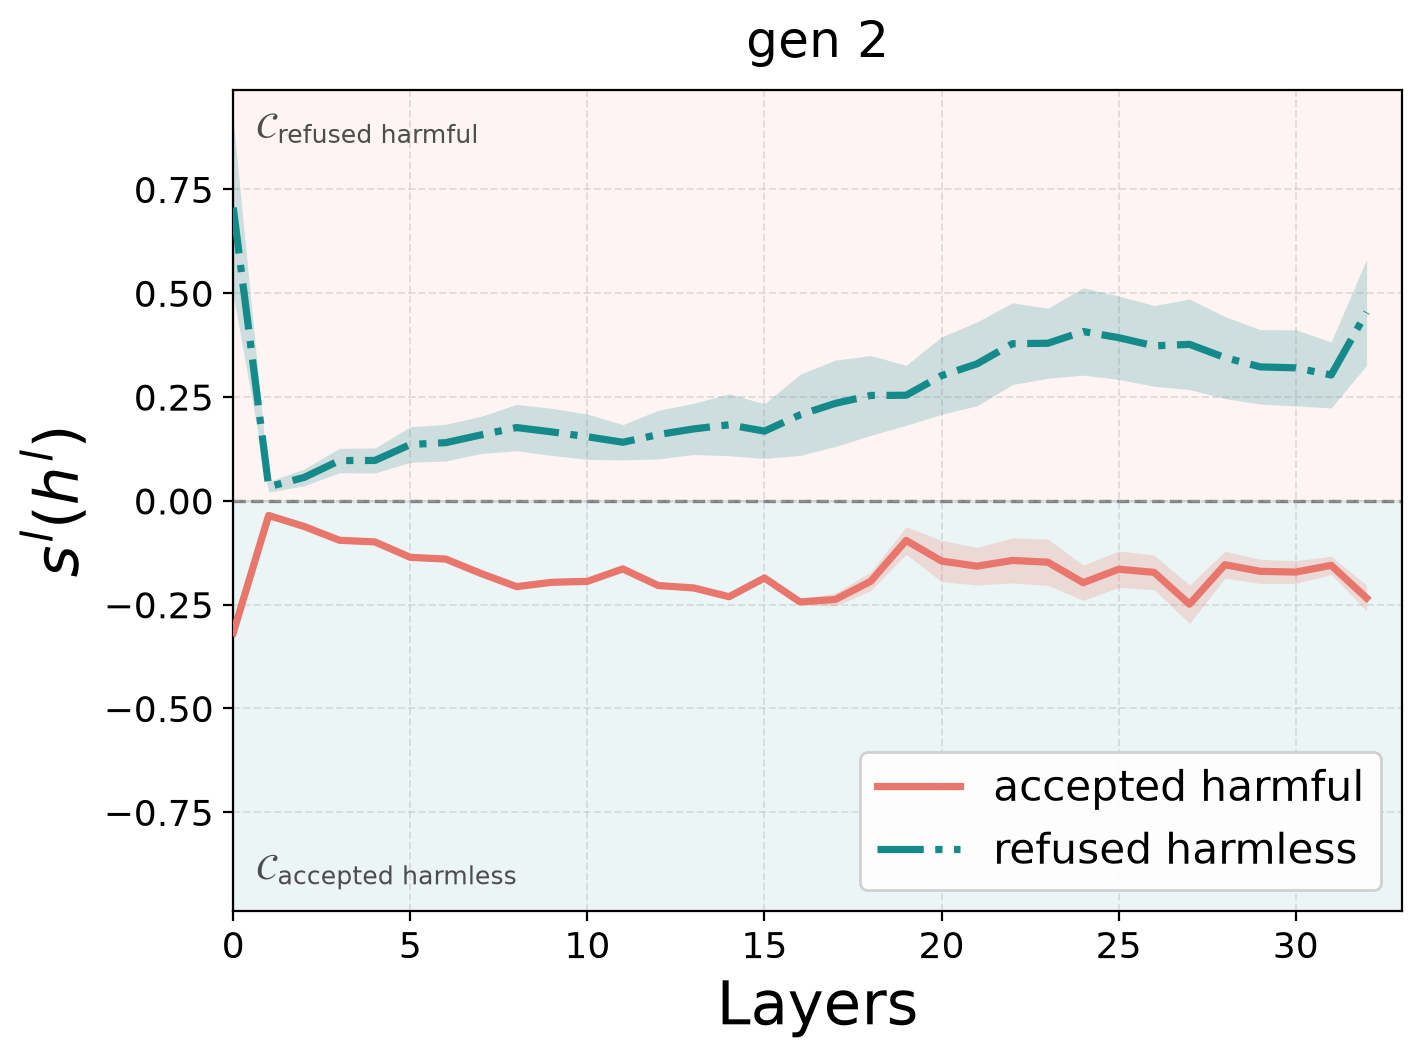
\includegraphics[width=\textwidth]{figures/nothink_run/08_slot22.png}
    \end{subfigure}
    \begin{subfigure}[b]{0.19\textwidth}
        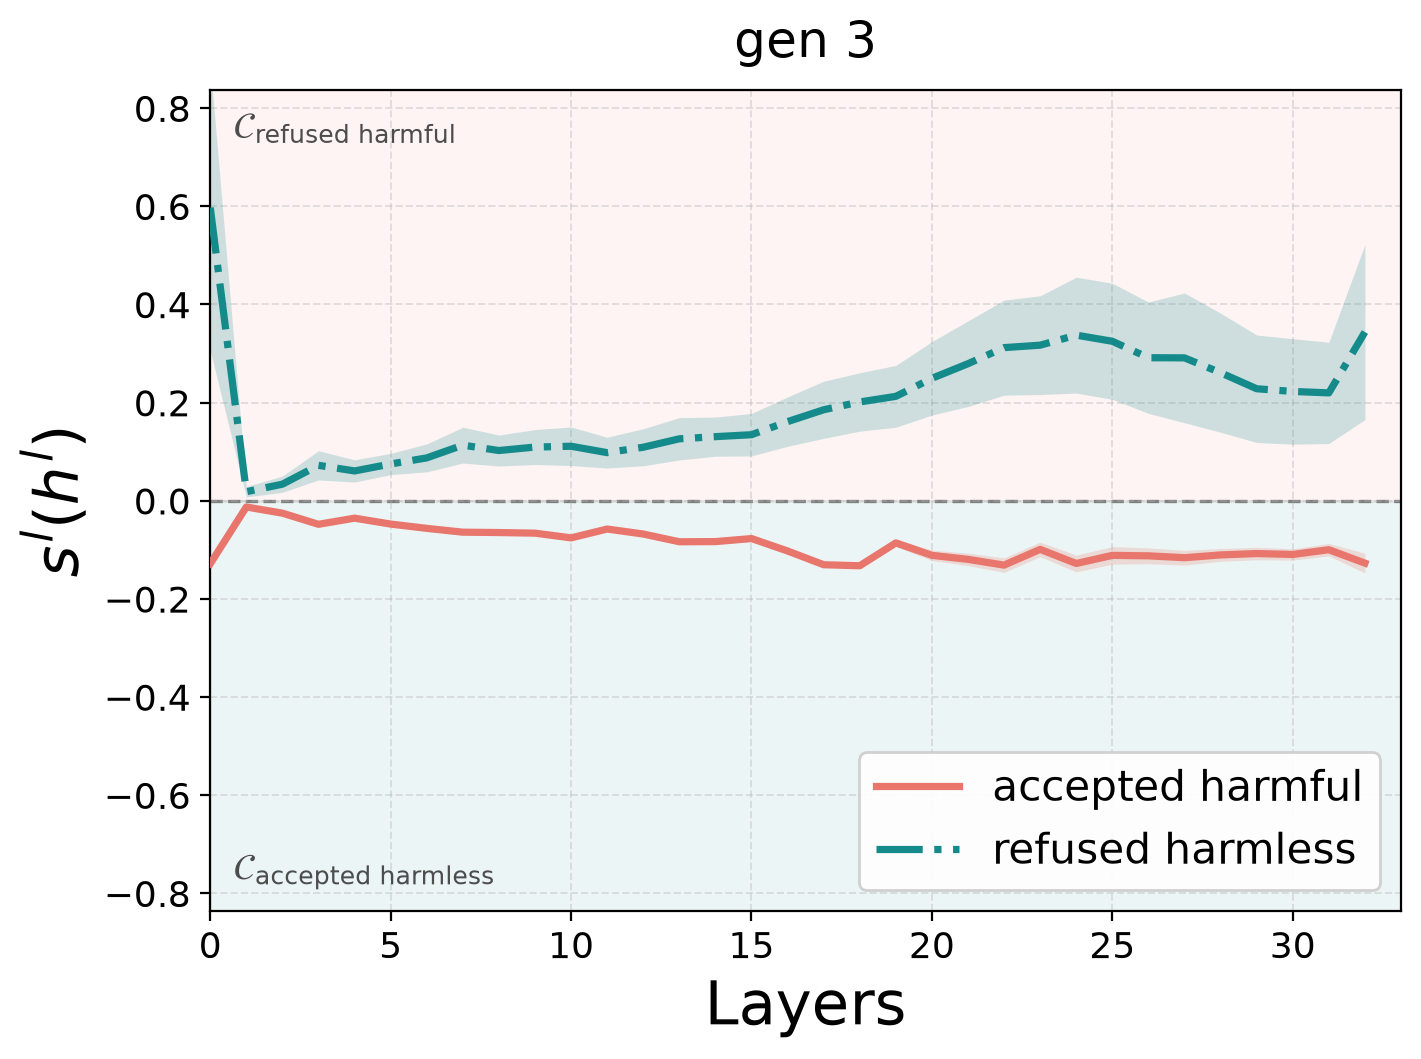
\includegraphics[width=\textwidth]{figures/nothink_run/09_slot23.png}
    \end{subfigure}

    \caption{No-think run.}
    \label{fig:app_nothink}
\end{figure*}


\begin{figure*}[htbp]
    \centering
    \begin{subfigure}[b]{0.19\textwidth}
        
\includegraphics[width=\textwidth]{figures/think_run/00_slot00.png}
    \end{subfigure}
    \begin{subfigure}[b]{0.19\textwidth}
        
\includegraphics[width=\textwidth]{figures/think_run/01_slot01.png}
    \end{subfigure}
    \begin{subfigure}[b]{0.19\textwidth}
        
\includegraphics[width=\textwidth]{figures/think_run/02_slot02.png}
    \end{subfigure}
    \begin{subfigure}[b]{0.19\textwidth}
        
\includegraphics[width=\textwidth]{figures/think_run/03_slot03.png}
    \end{subfigure}
    \begin{subfigure}[b]{0.19\textwidth}
        
\includegraphics[width=\textwidth]{figures/think_run/04_slot04.png}
    \end{subfigure}

    \vspace{0.5em}

    \begin{subfigure}[b]{0.19\textwidth}
        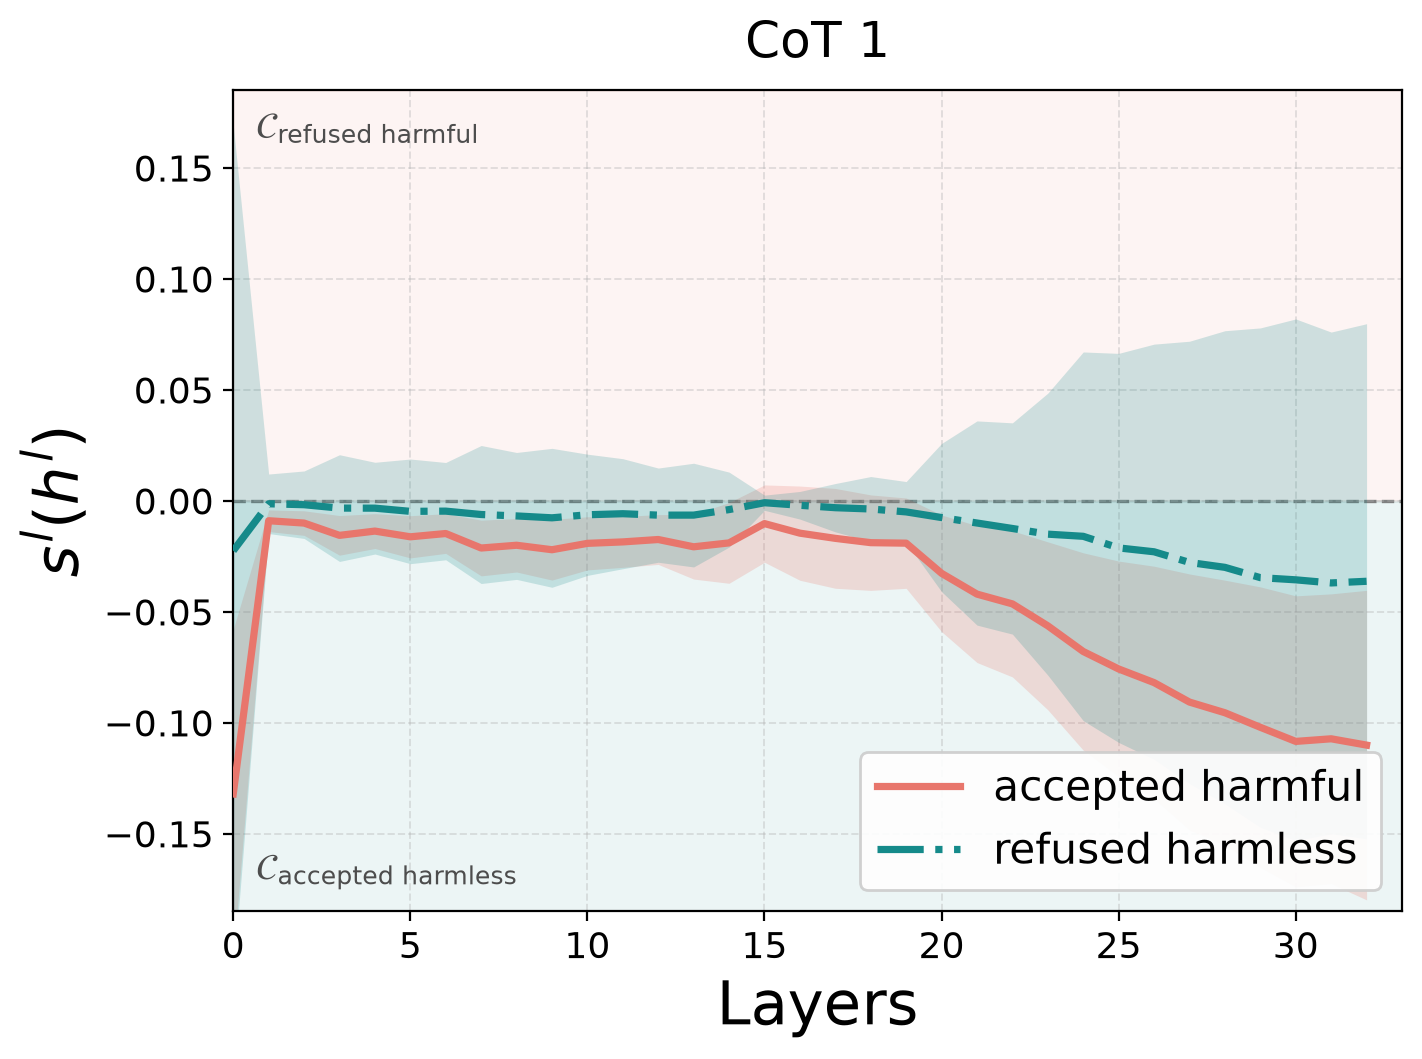
\includegraphics[width=\textwidth]{figures/think_run/05_slot05.png}
    \end{subfigure}
    \begin{subfigure}[b]{0.19\textwidth}
        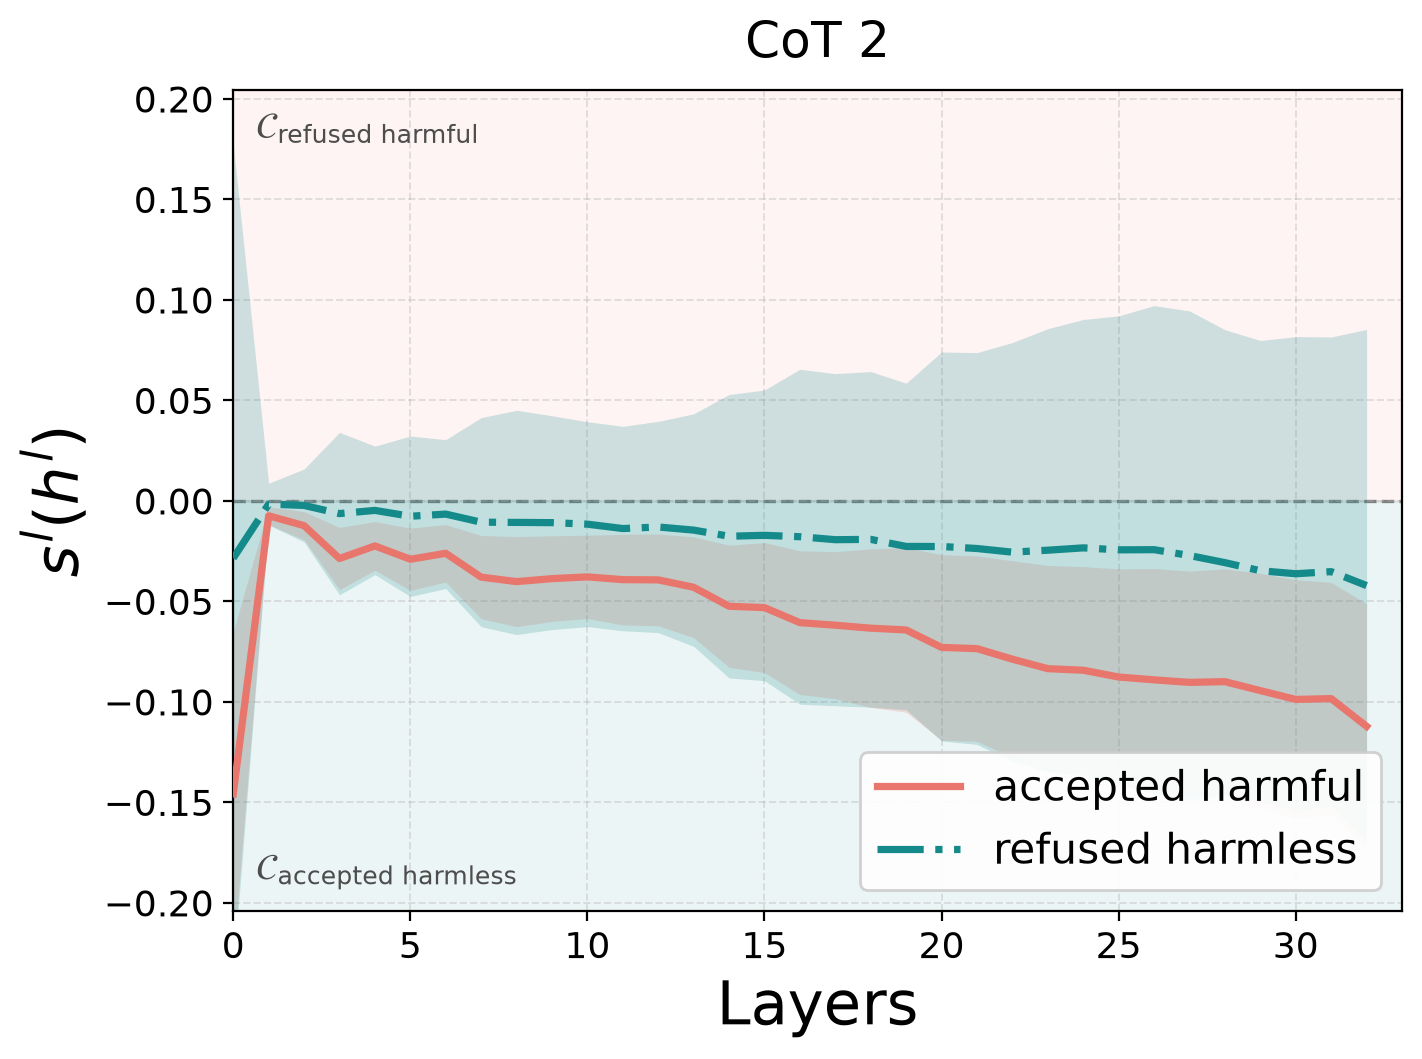
\includegraphics[width=\textwidth]{figures/think_run/06_slot06.png}
    \end{subfigure}
    \begin{subfigure}[b]{0.19\textwidth}
        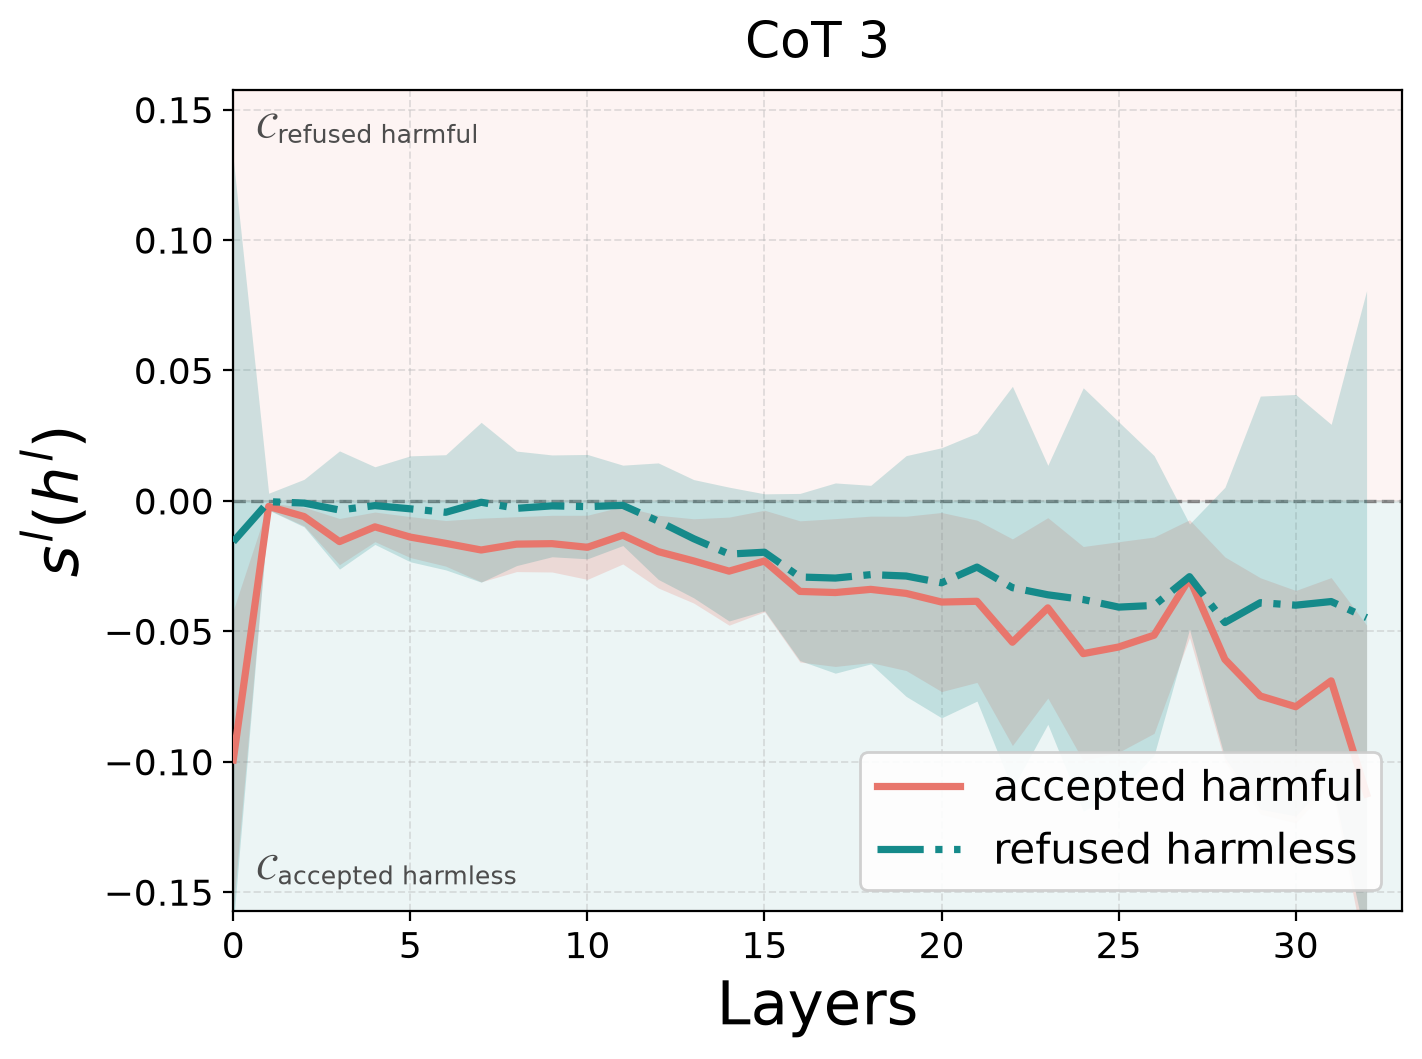
\includegraphics[width=\textwidth]{figures/think_run/07_slot07.png}
    \end{subfigure}
    \begin{subfigure}[b]{0.19\textwidth}
        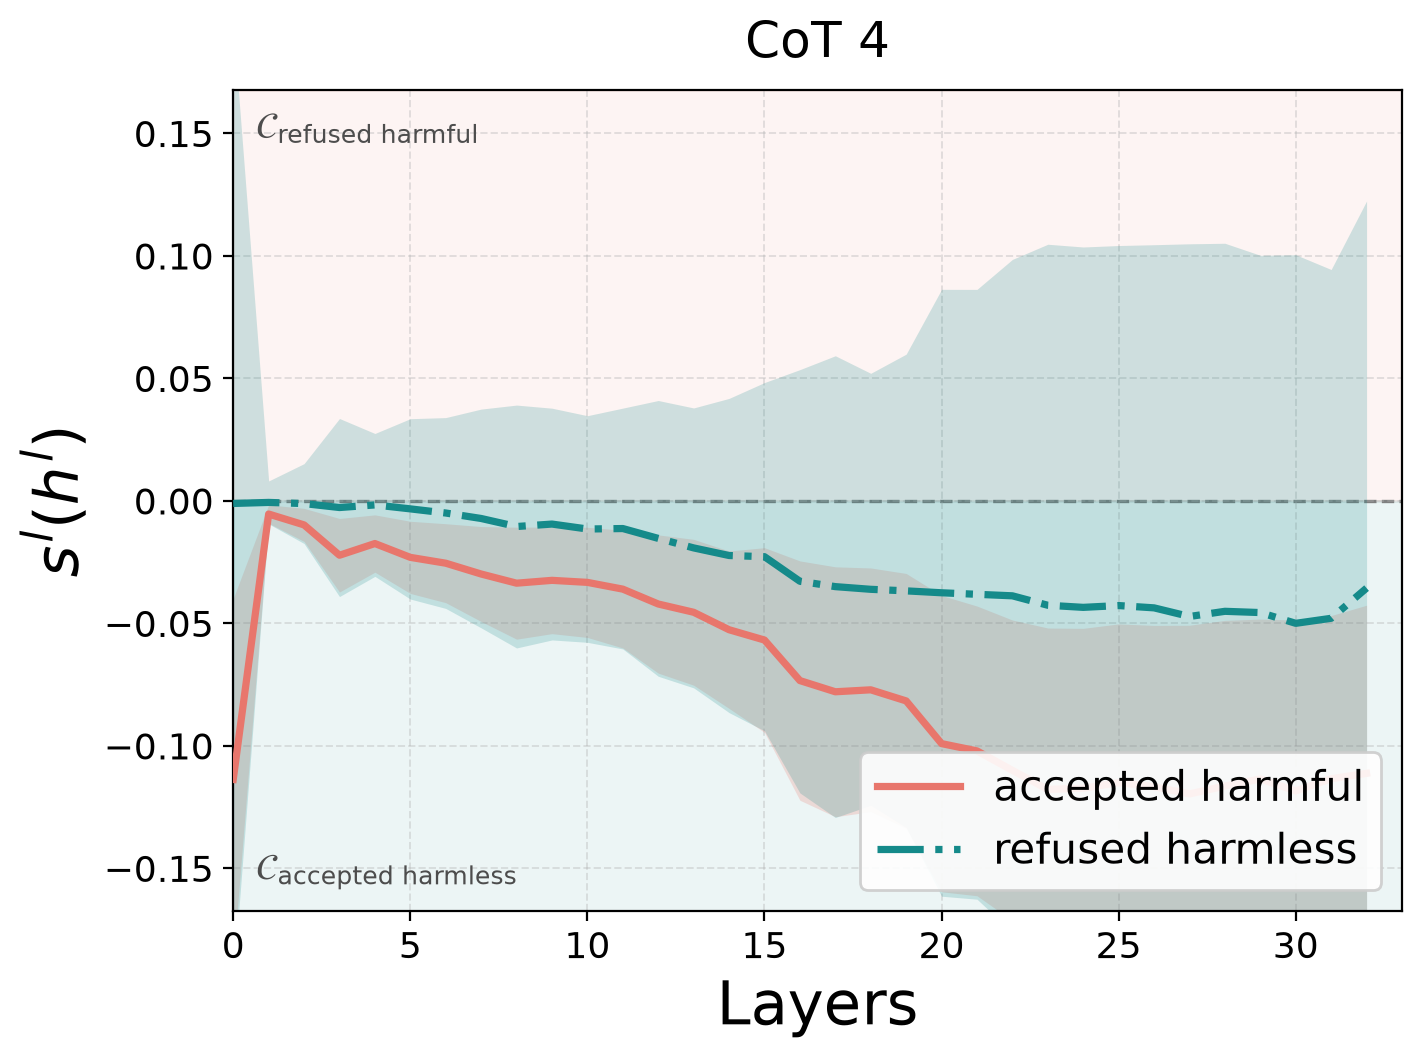
\includegraphics[width=\textwidth]{figures/think_run/08_slot08.png}
    \end{subfigure}
    \begin{subfigure}[b]{0.19\textwidth}
        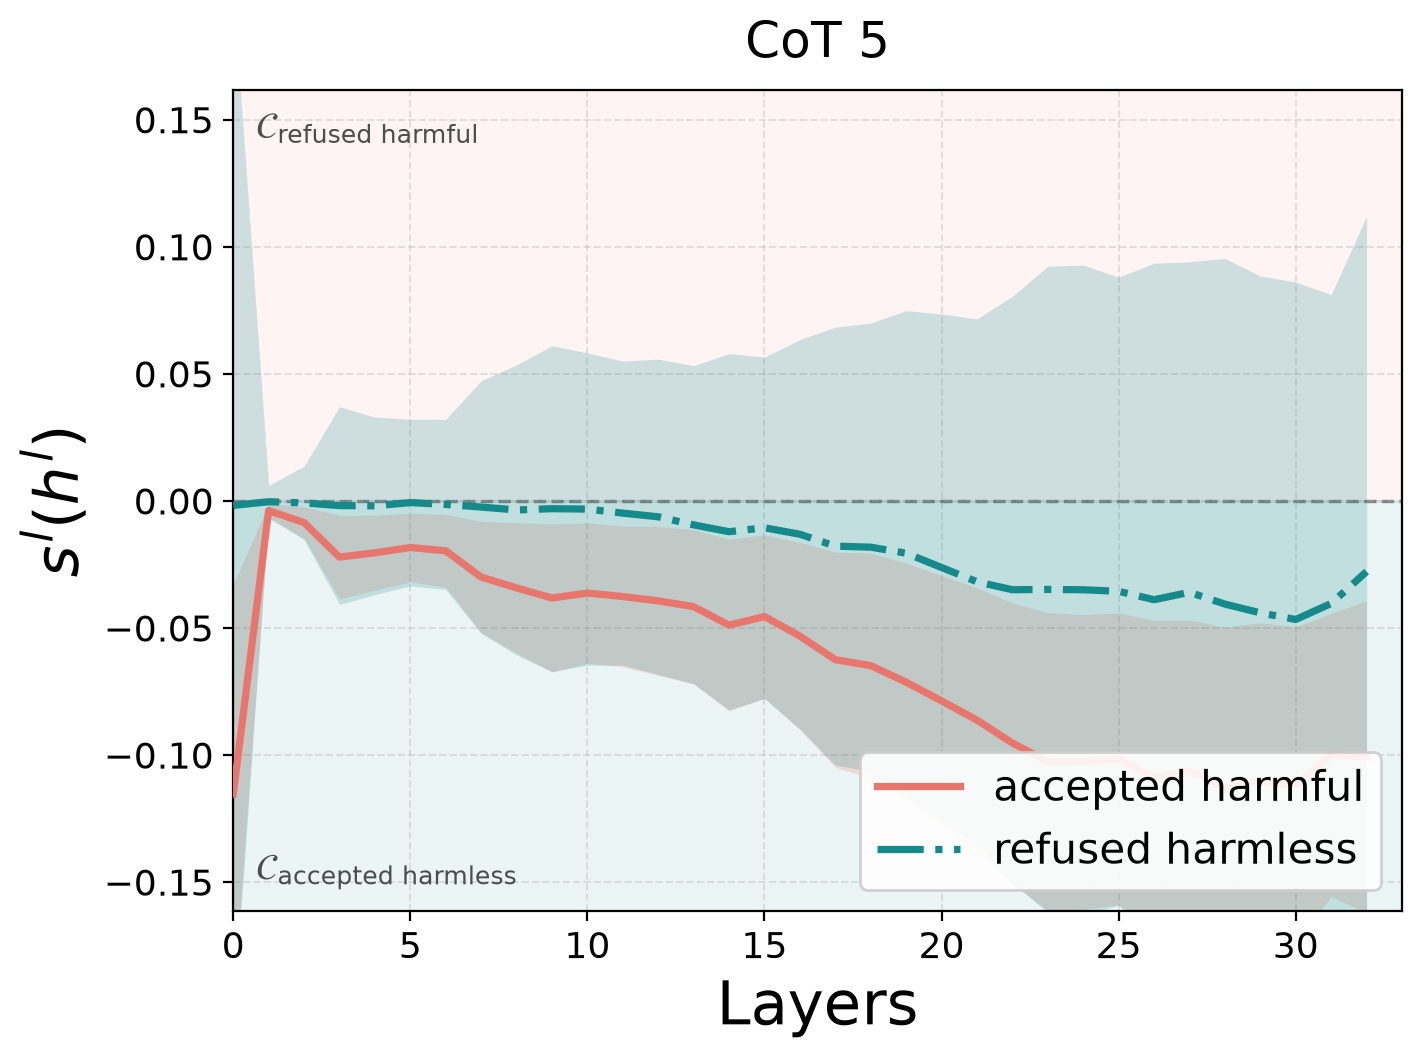
\includegraphics[width=\textwidth]{figures/think_run/09_slot09.png}
    \end{subfigure}

    \vspace{0.5em}

    \begin{subfigure}[b]{0.19\textwidth}
        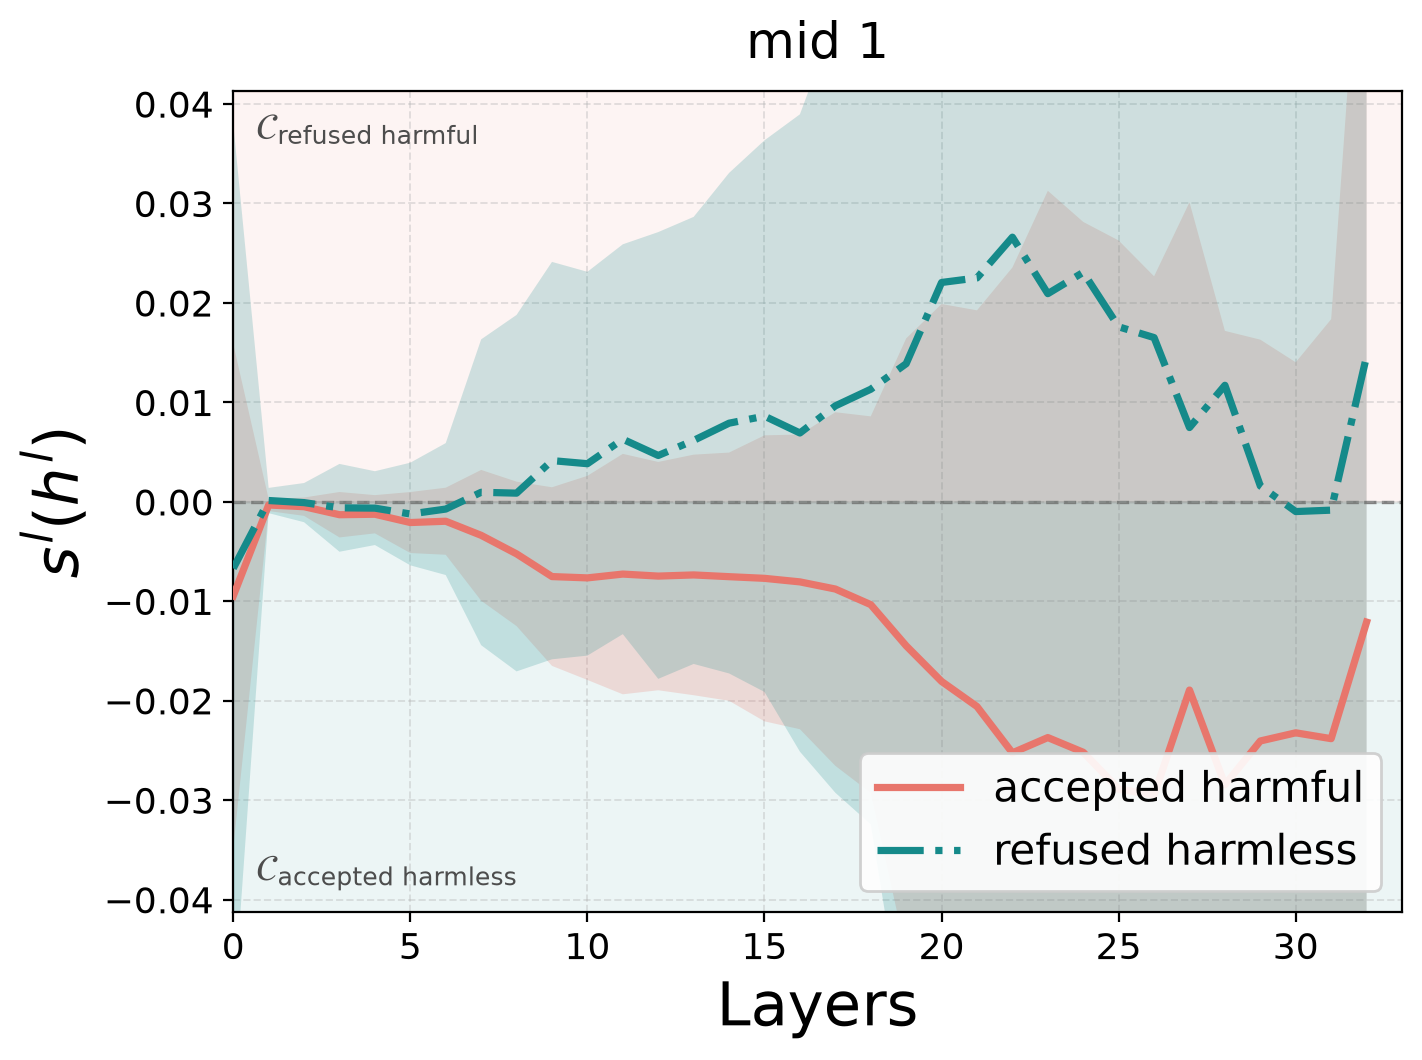
\includegraphics[width=\textwidth]{figures/think_run/10_slot10.png}
    \end{subfigure}
    \begin{subfigure}[b]{0.19\textwidth}
        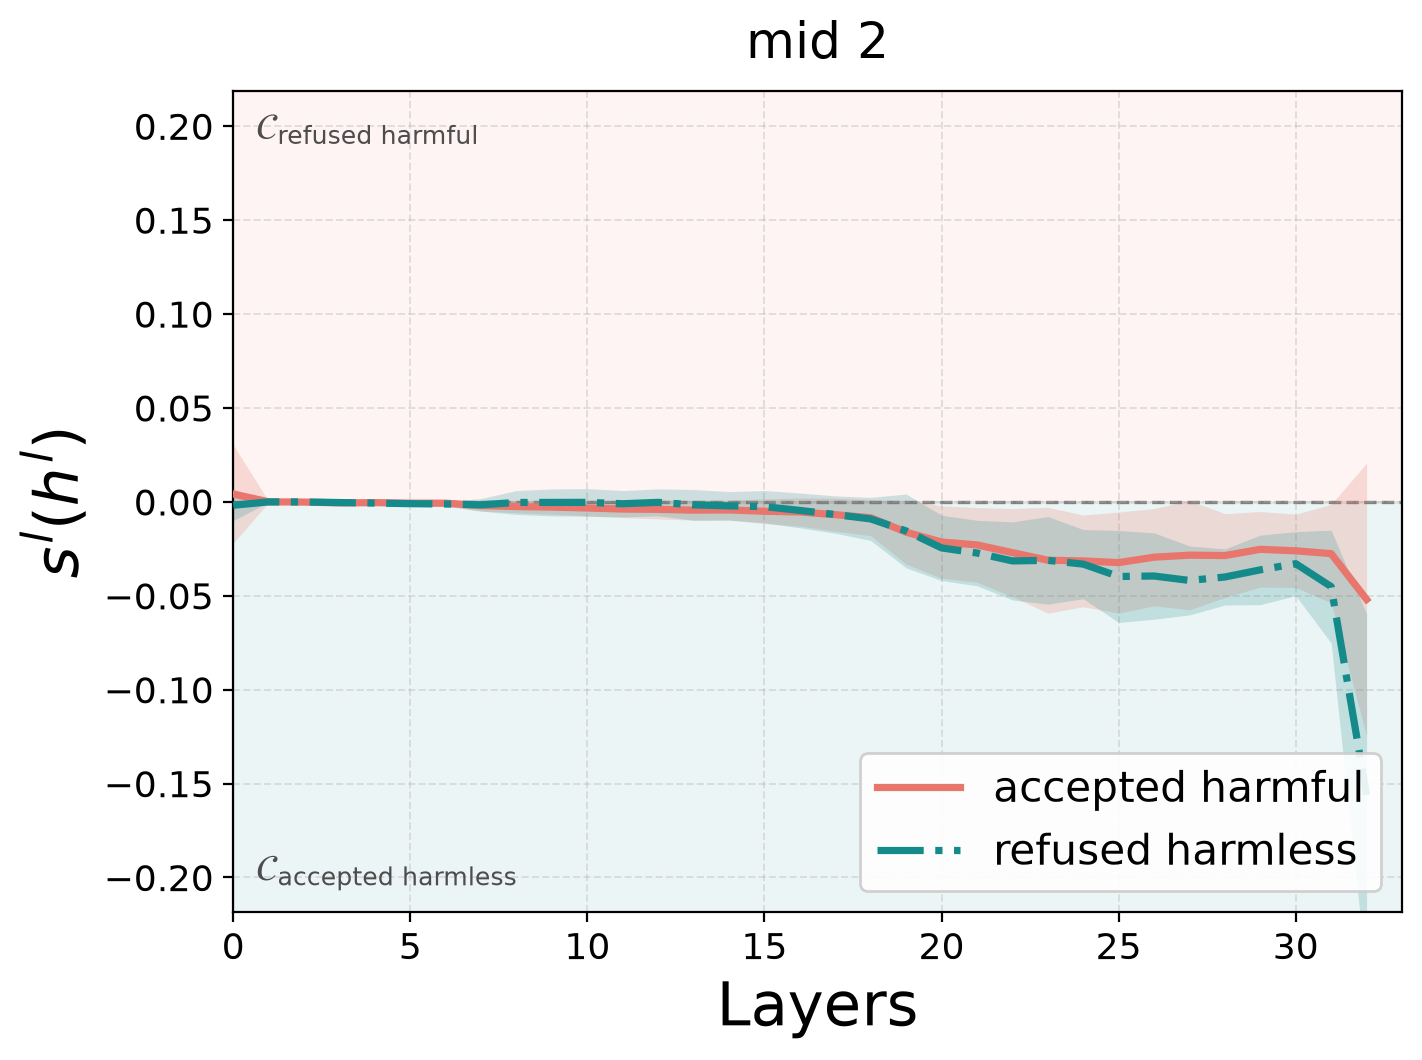
\includegraphics[width=\textwidth]{figures/think_run/11_slot11.png}
    \end{subfigure}
    \begin{subfigure}[b]{0.19\textwidth}
        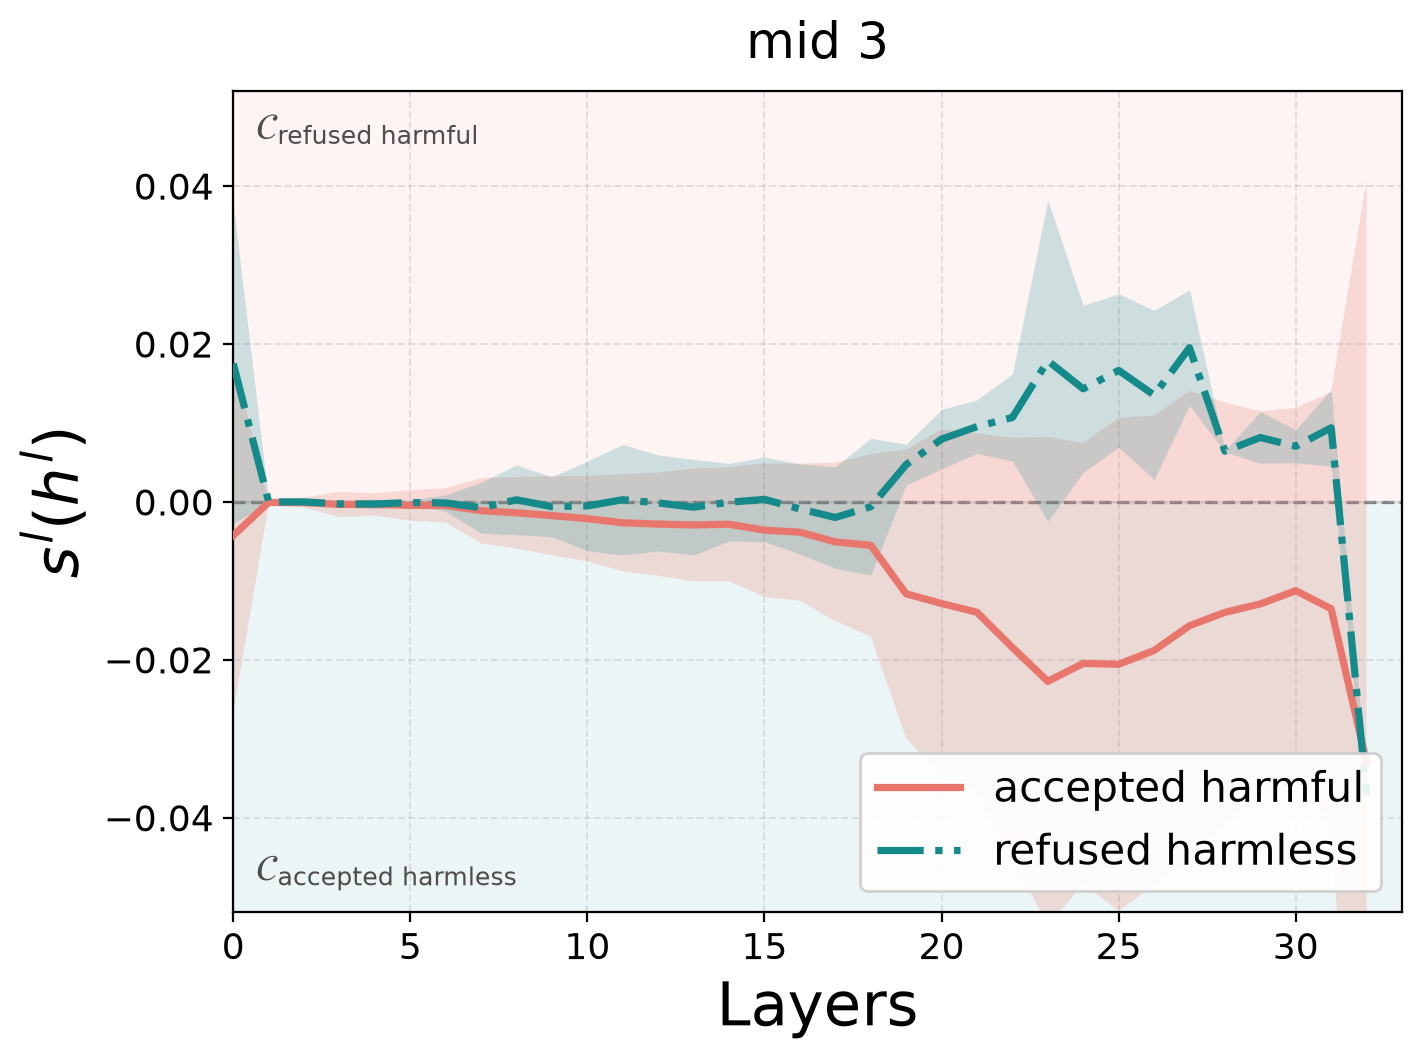
\includegraphics[width=\textwidth]{figures/think_run/12_slot12.png}
    \end{subfigure}
    \begin{subfigure}[b]{0.19\textwidth}
        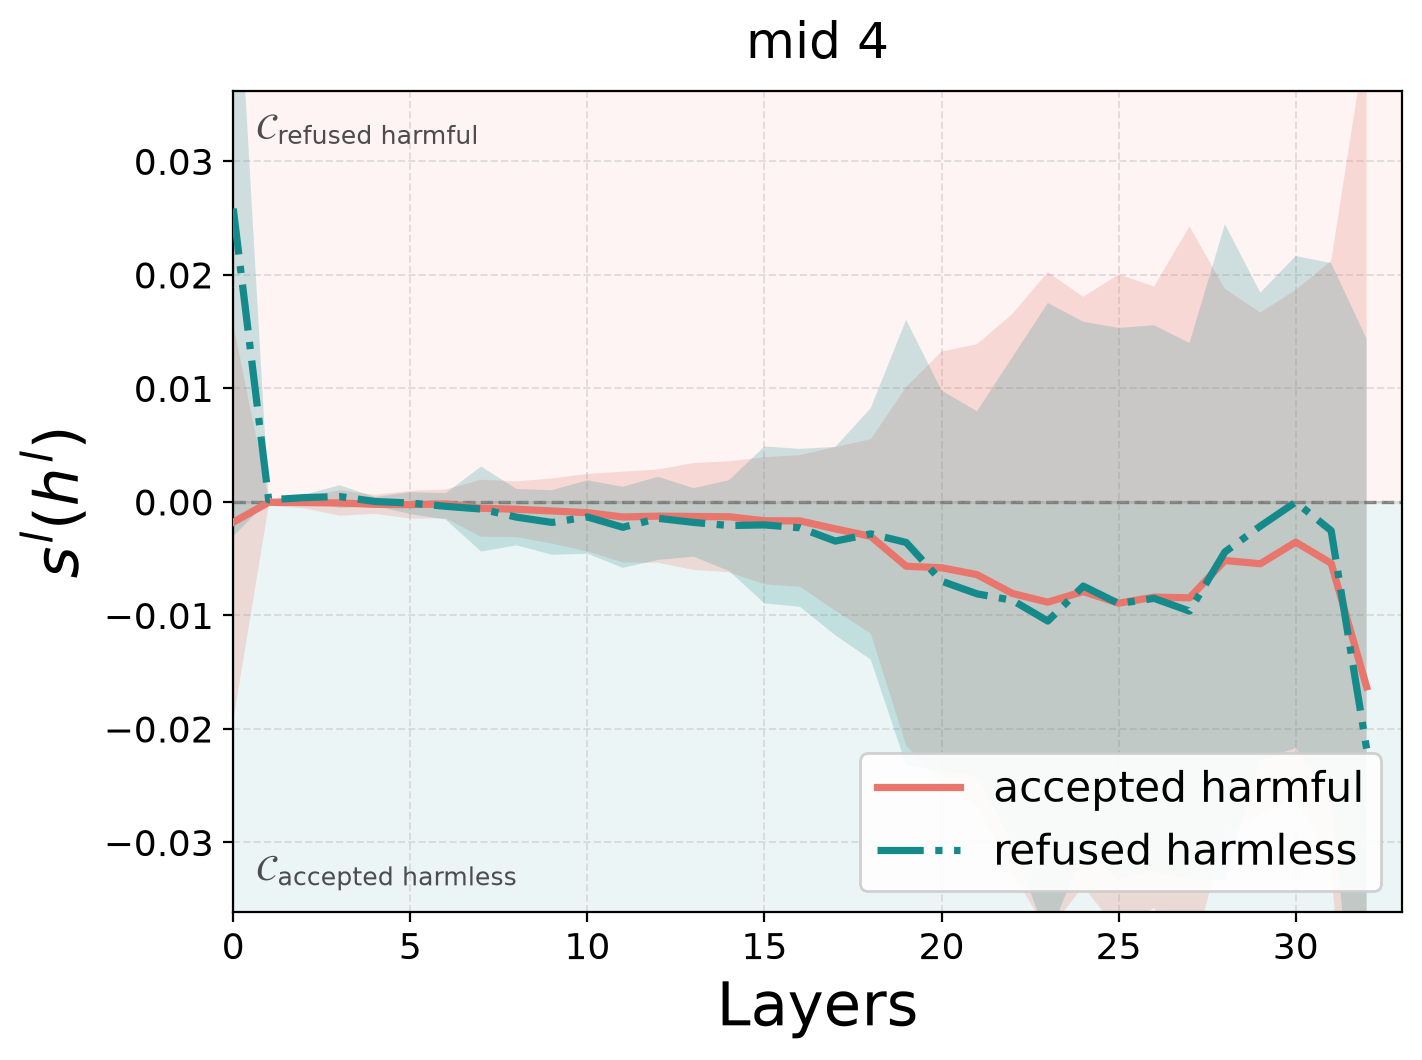
\includegraphics[width=\textwidth]{figures/think_run/13_slot13.png}
    \end{subfigure}
    \begin{subfigure}[b]{0.19\textwidth}
        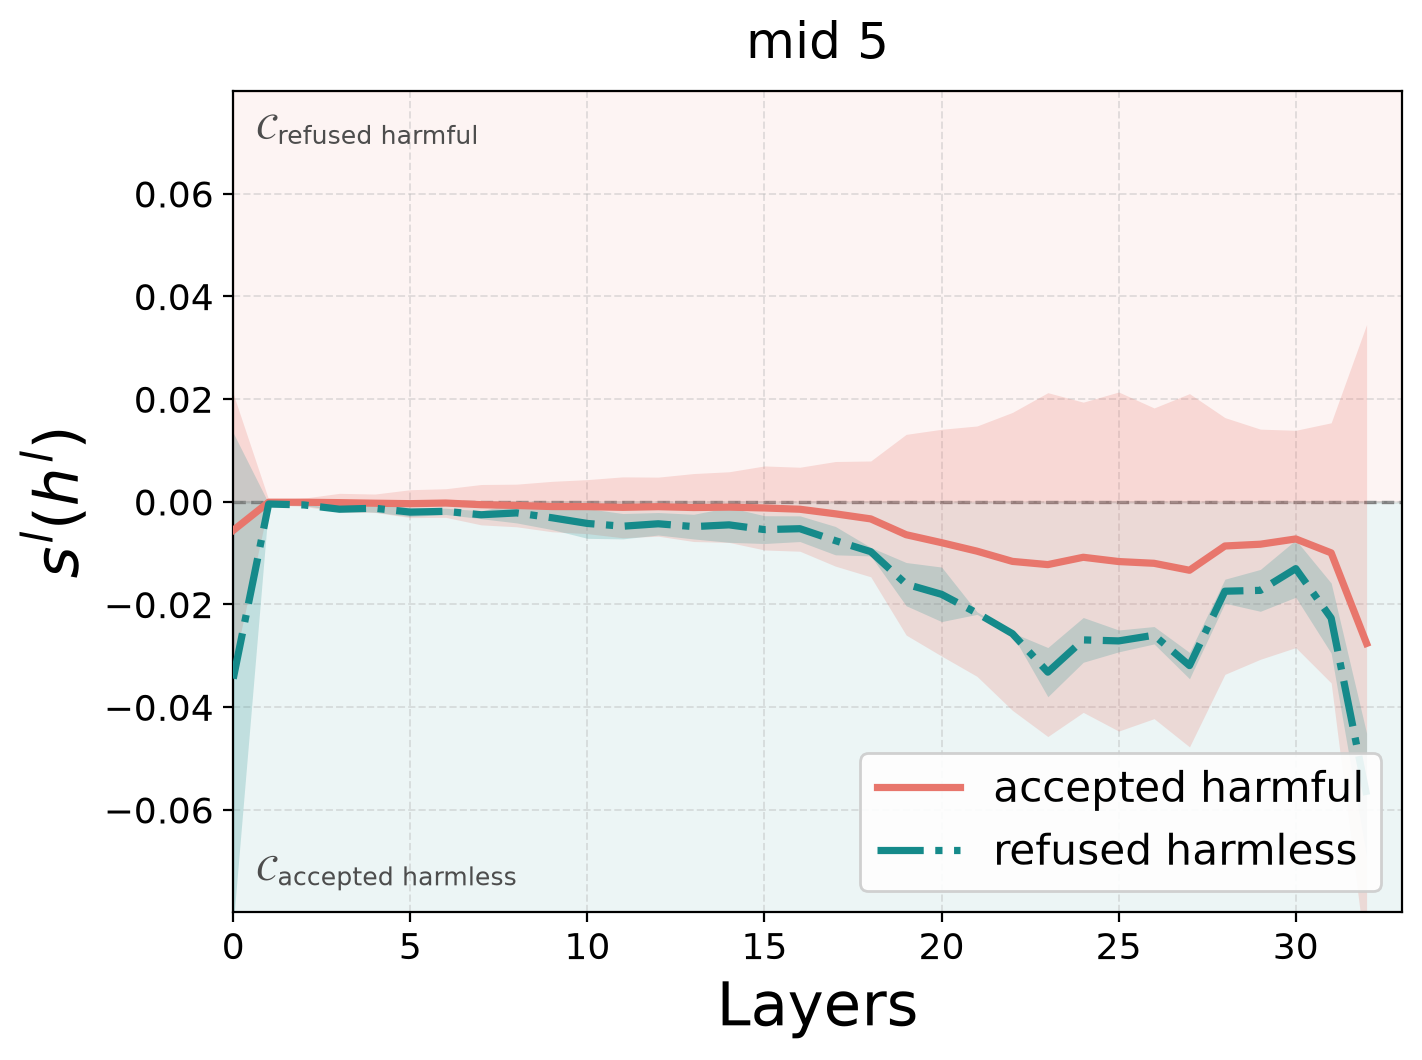
\includegraphics[width=\textwidth]{figures/think_run/14_slot14.png}
    \end{subfigure}

    \vspace{0.5em}

    \begin{subfigure}[b]{0.19\textwidth}
        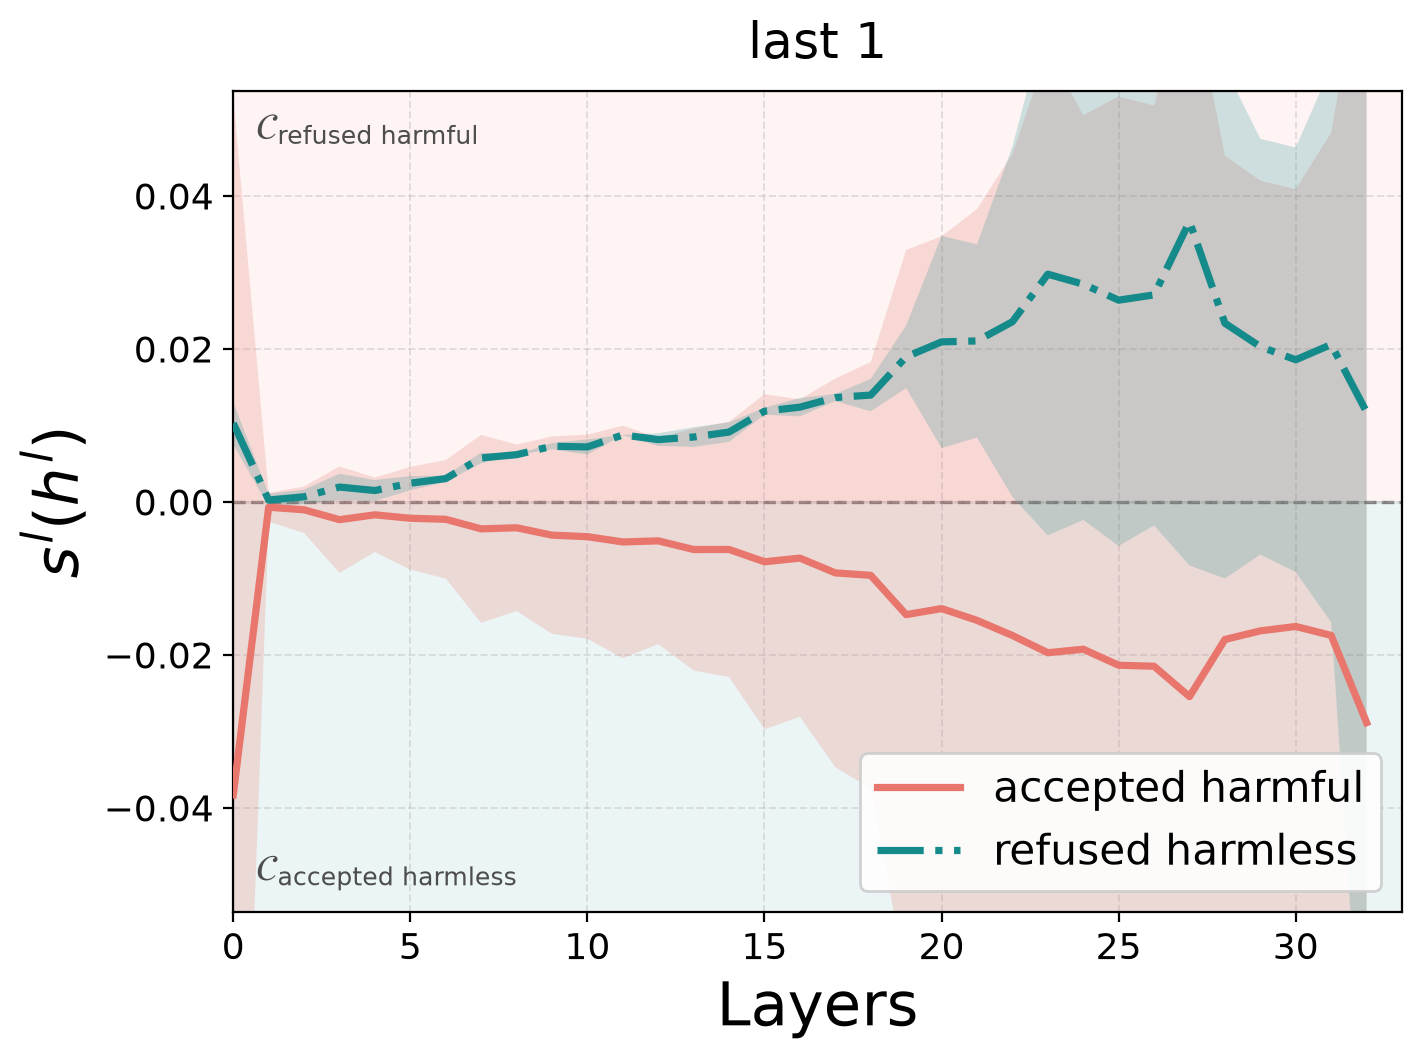
\includegraphics[width=\textwidth]{figures/think_run/15_slot15.png}
    \end{subfigure}
    \begin{subfigure}[b]{0.19\textwidth}
        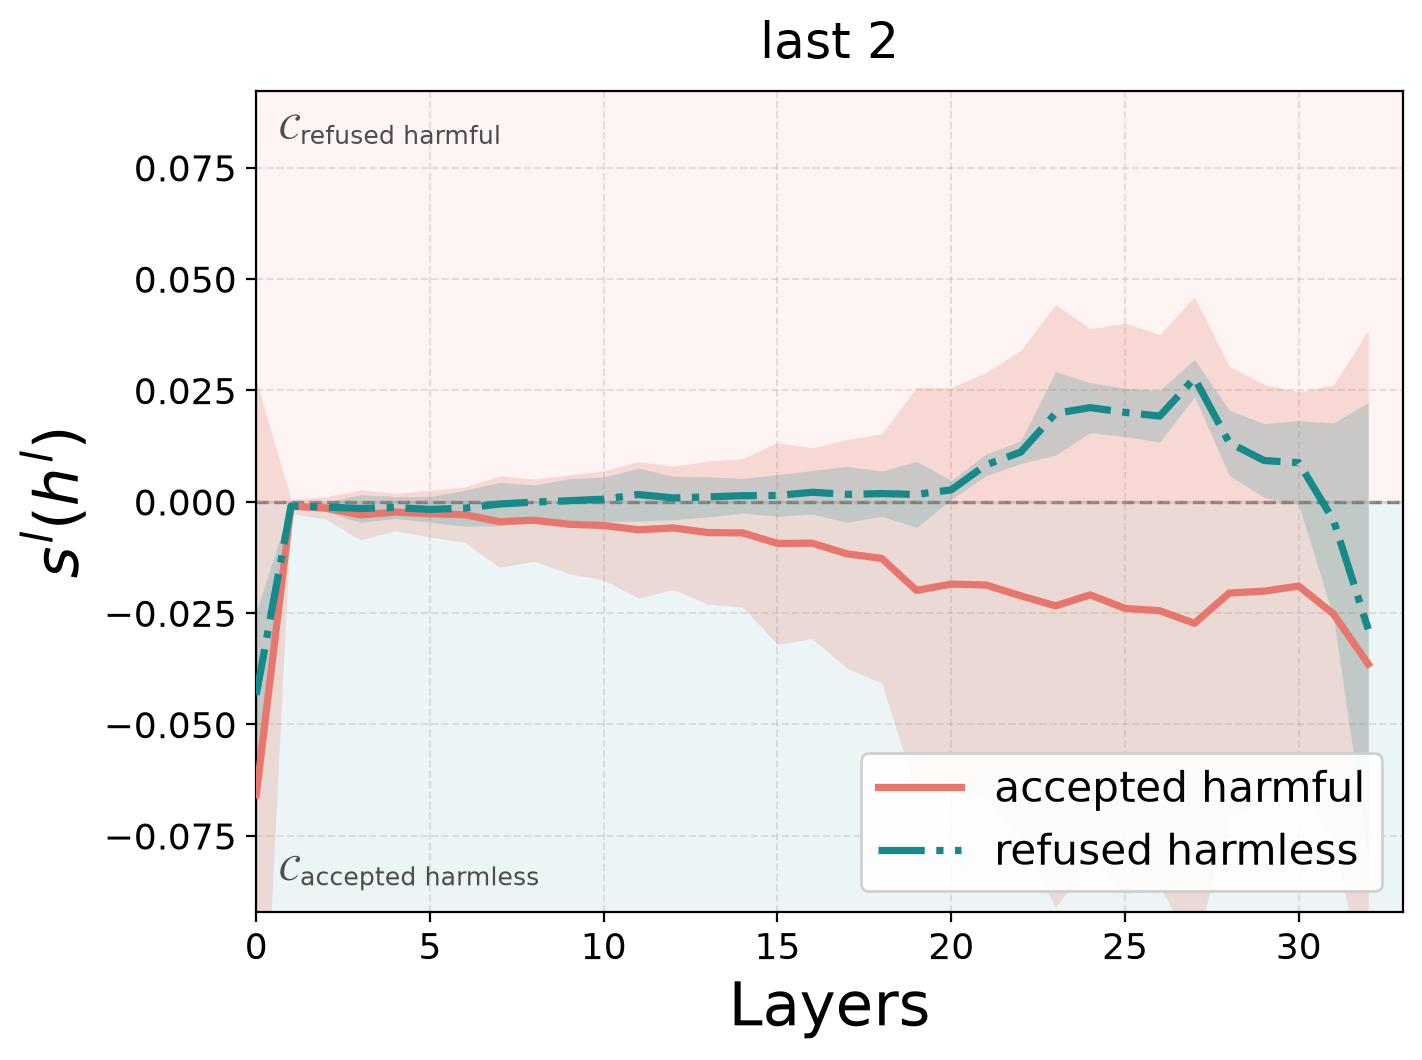
\includegraphics[width=\textwidth]{figures/think_run/16_slot16.png}
    \end{subfigure}
    \begin{subfigure}[b]{0.19\textwidth}
        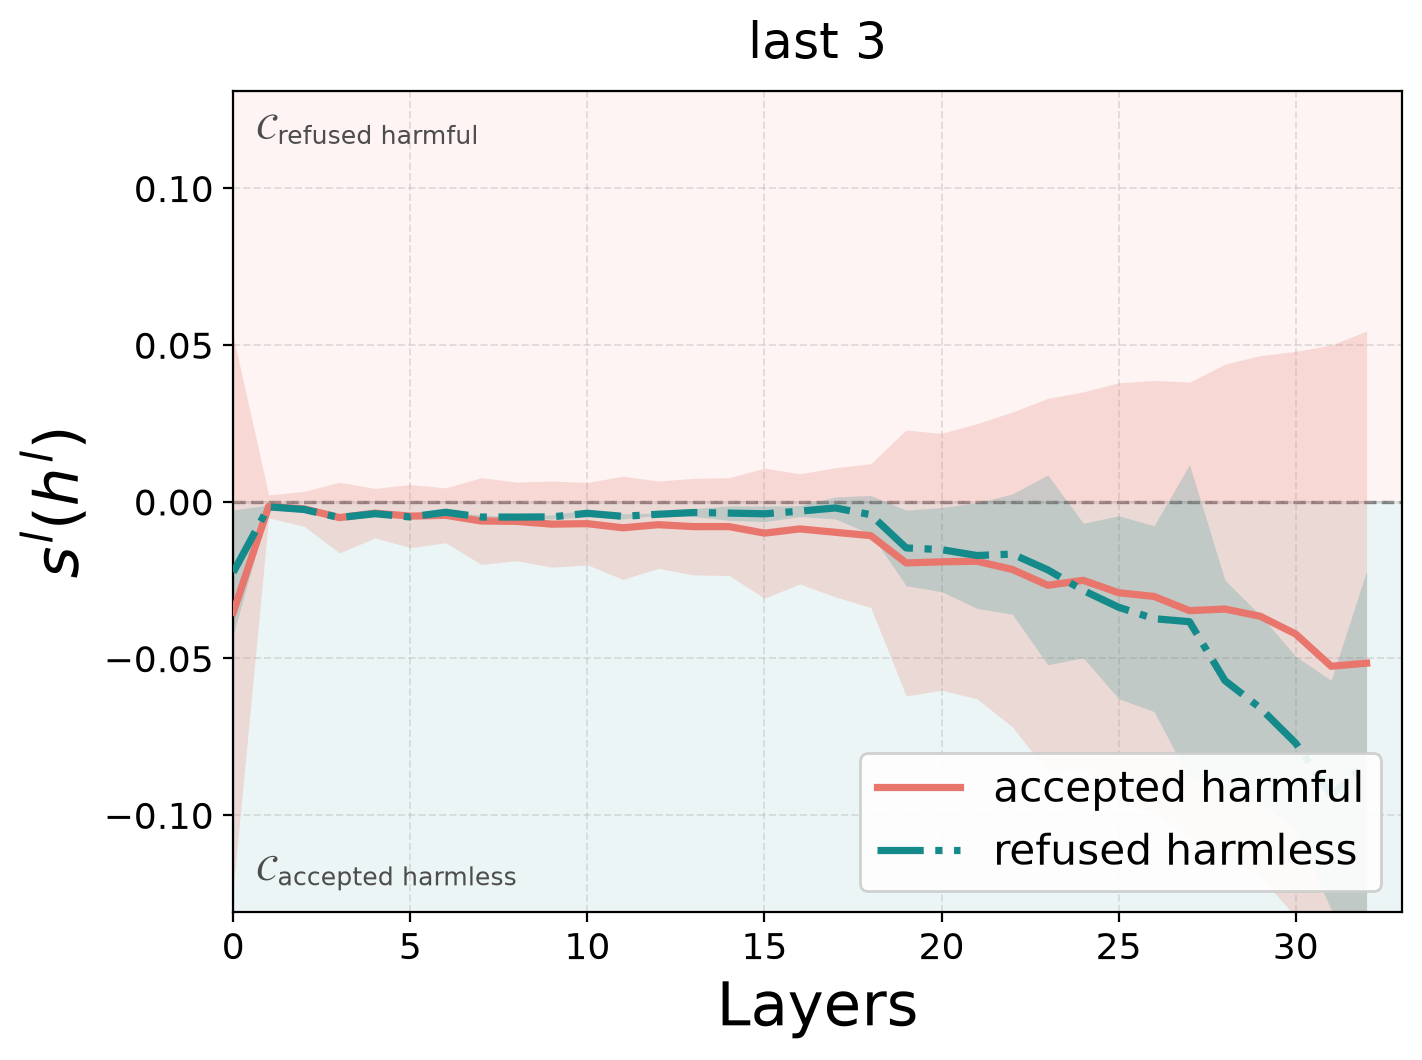
\includegraphics[width=\textwidth]{figures/think_run/17_slot17.png}
    \end{subfigure}
    \begin{subfigure}[b]{0.19\textwidth}
        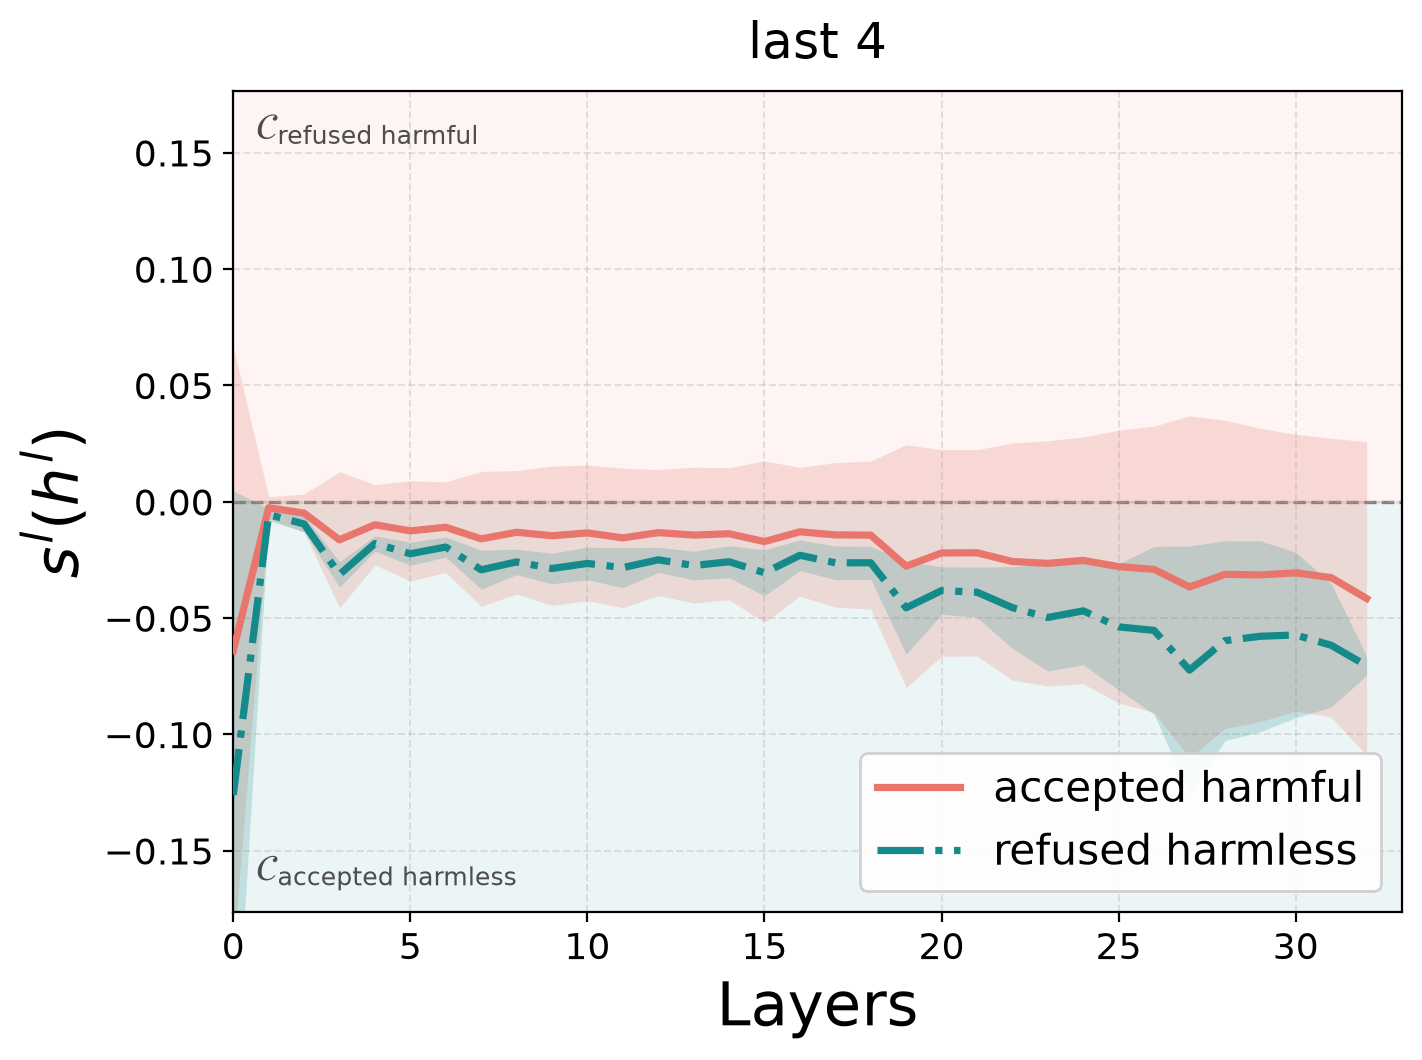
\includegraphics[width=\textwidth]{figures/think_run/18_slot18.png}
    \end{subfigure}
    \begin{subfigure}[b]{0.19\textwidth}
        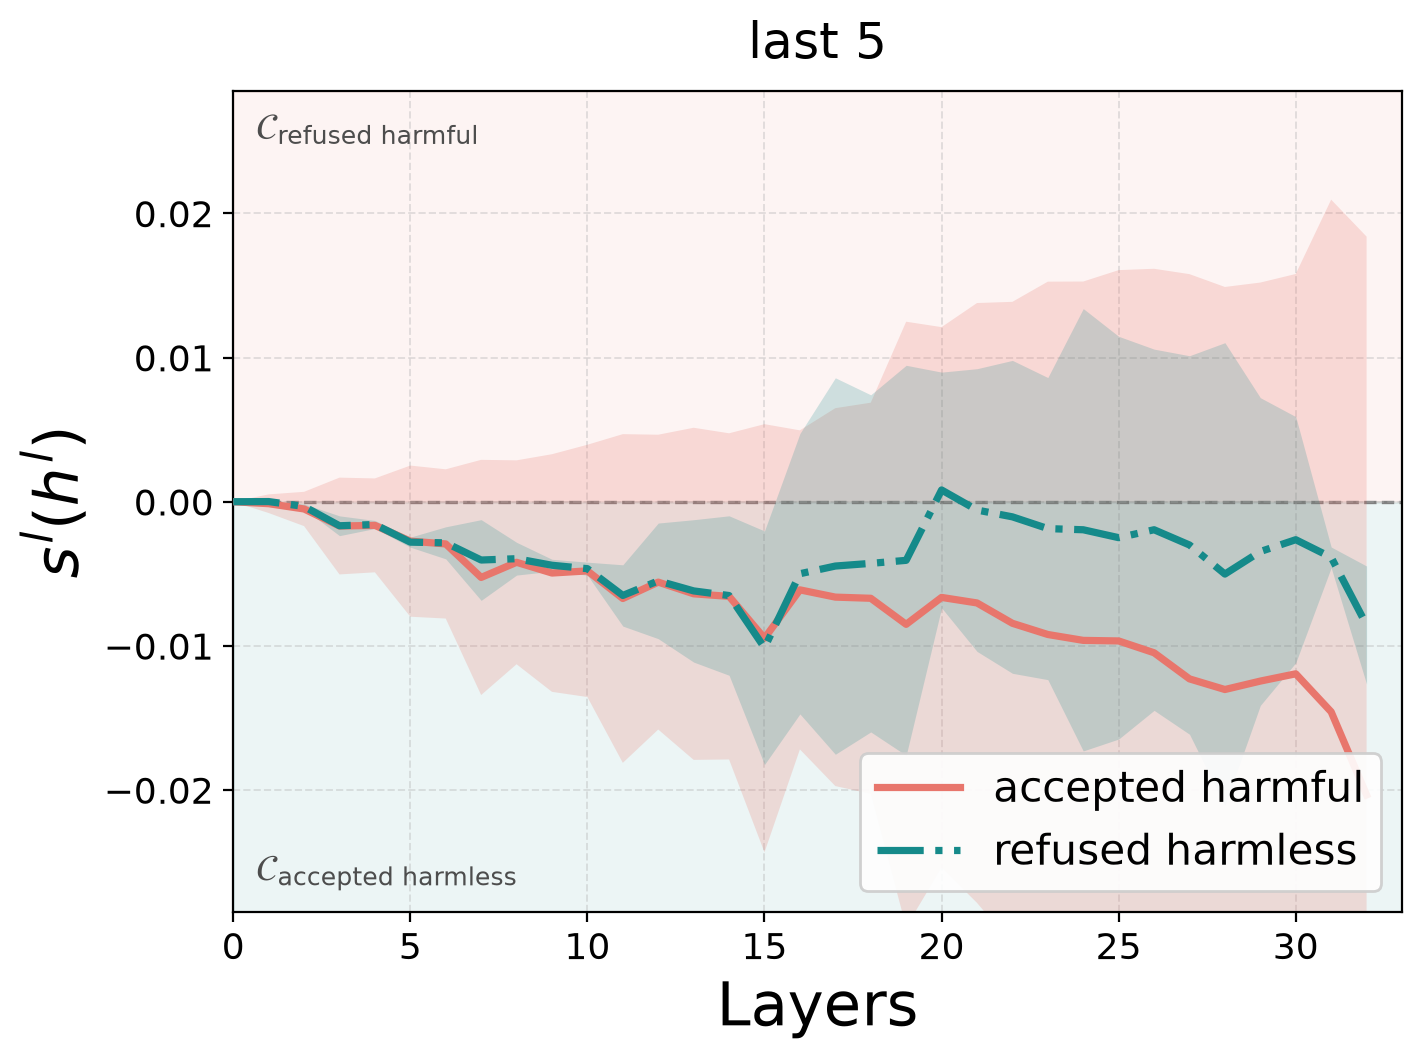
\includegraphics[width=\textwidth]{figures/think_run/19_slot19.png}
    \end{subfigure}

    \vspace{0.5em}

    \begin{subfigure}[b]{0.19\textwidth}
        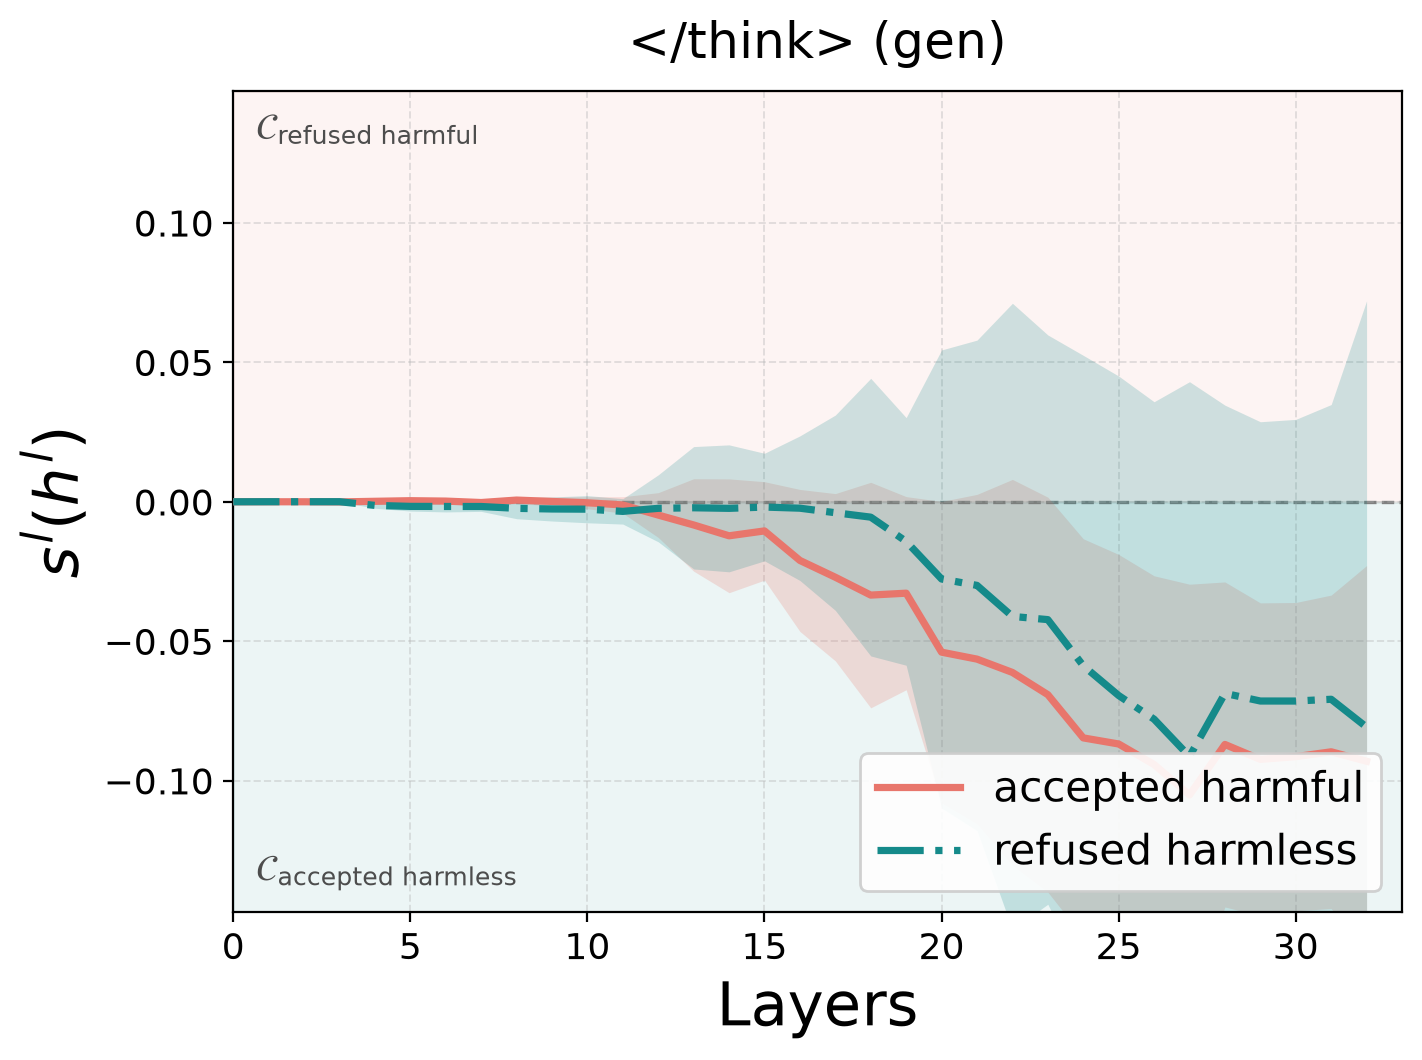
\includegraphics[width=\textwidth]{figures/think_run/20_slot24.png}
    \end{subfigure}
    \begin{subfigure}[b]{0.19\textwidth}
        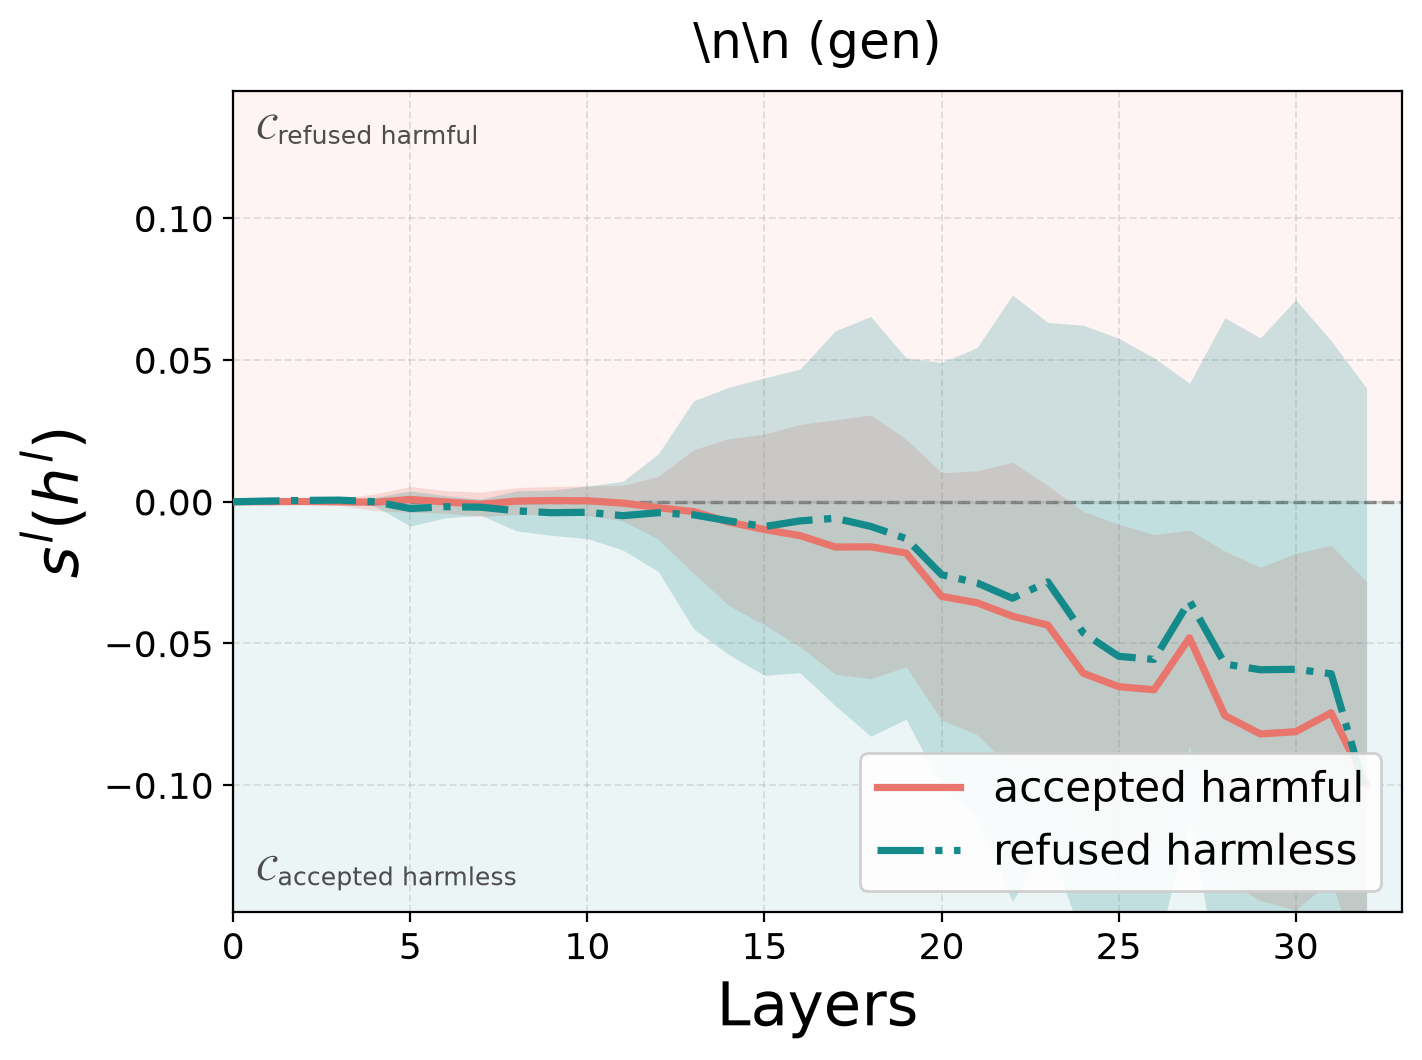
\includegraphics[width=\textwidth]{figures/think_run/21_slot20.png}
    \end{subfigure}
    \begin{subfigure}[b]{0.19\textwidth}
        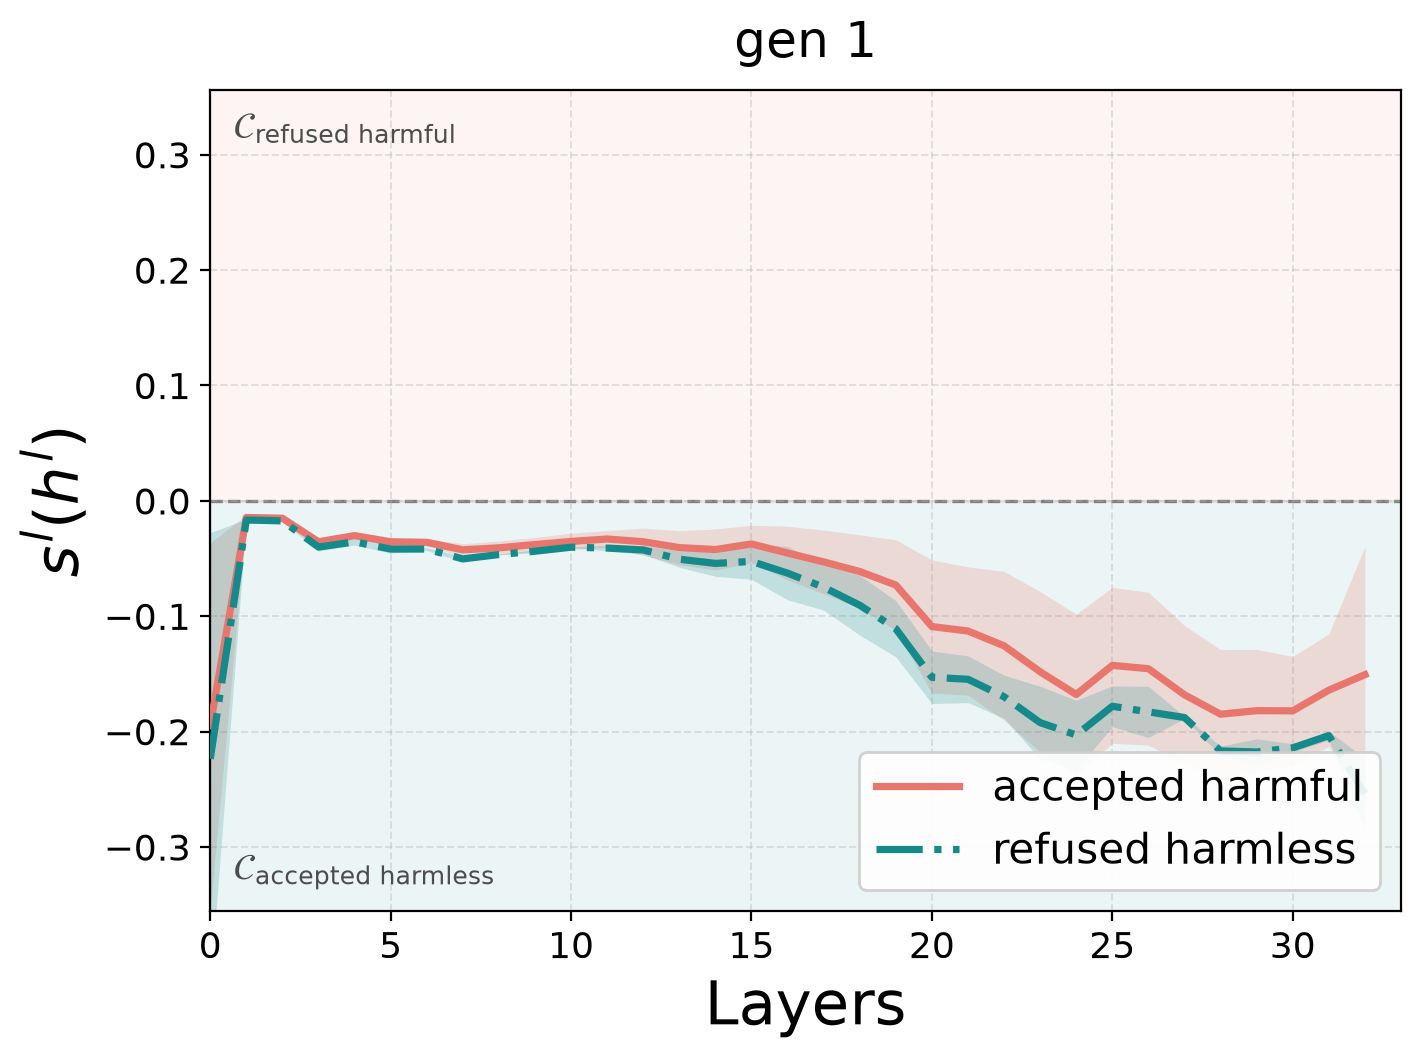
\includegraphics[width=\textwidth]{figures/think_run/22_slot21.png}
    \end{subfigure}
    \begin{subfigure}[b]{0.19\textwidth}
        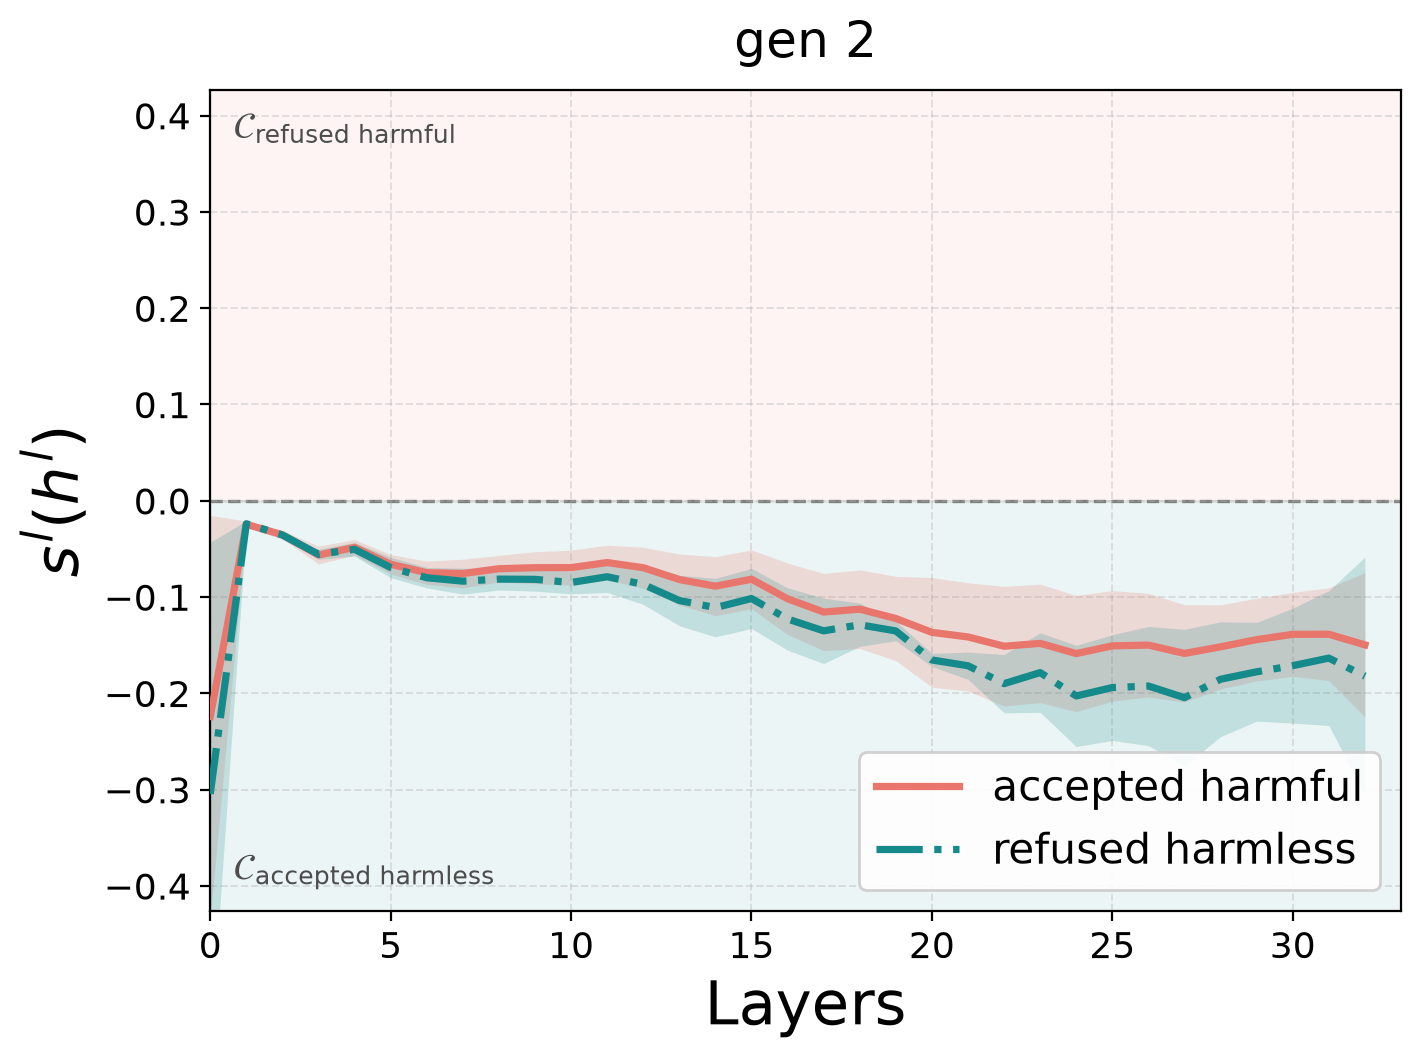
\includegraphics[width=\textwidth]{figures/think_run/23_slot22.png}
    \end{subfigure}
    \begin{subfigure}[b]{0.19\textwidth}
        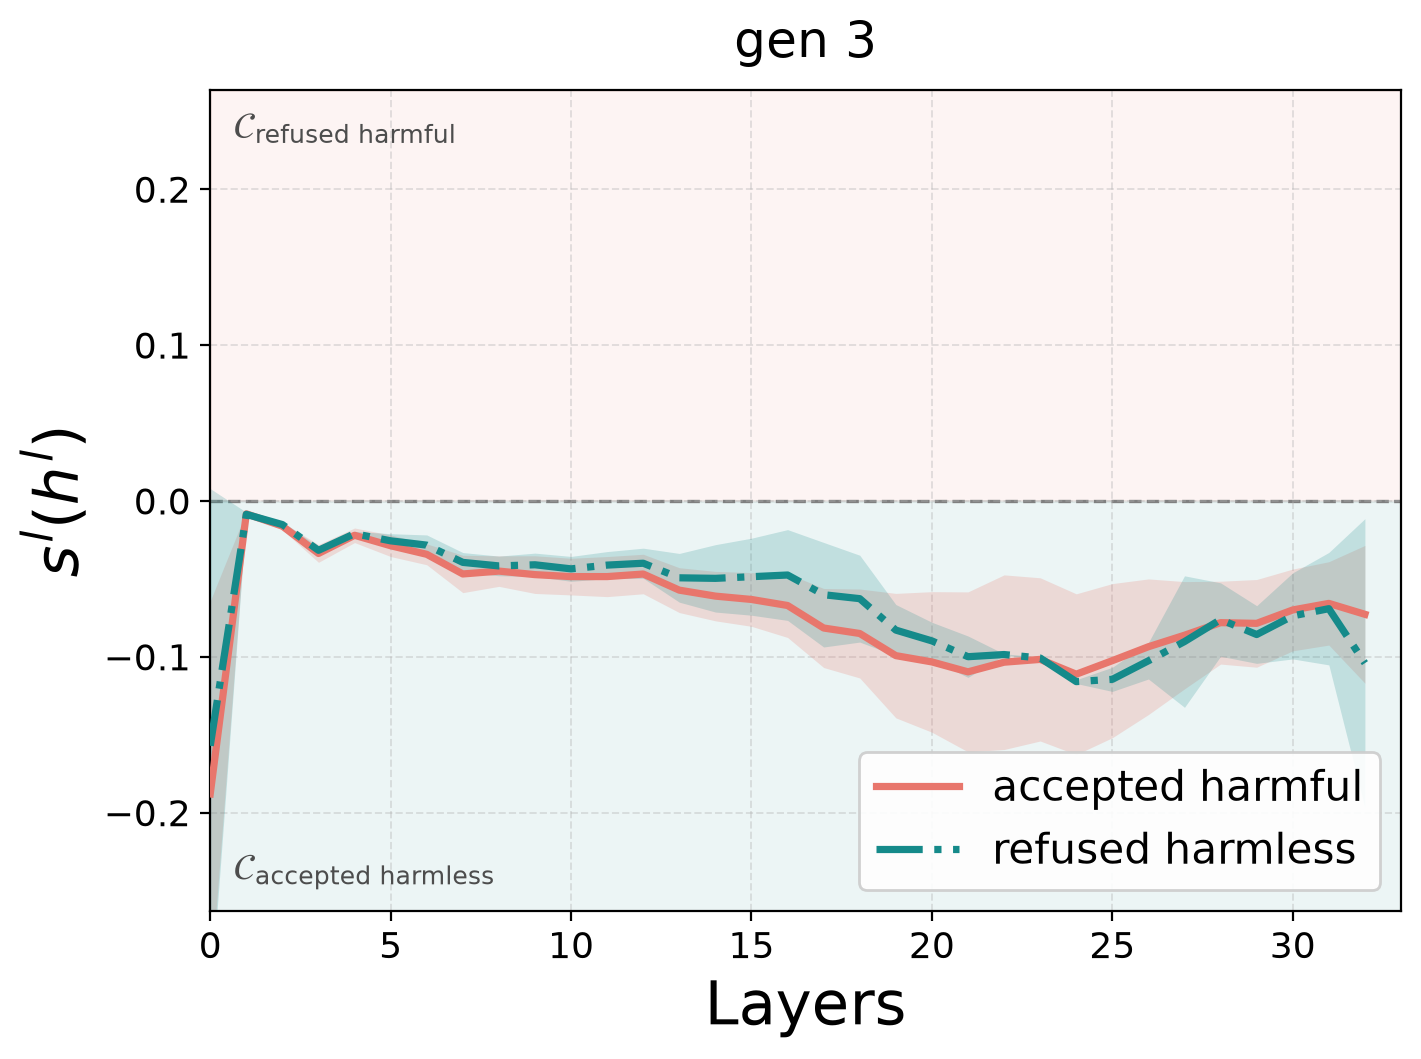
\includegraphics[width=\textwidth]{figures/think_run/24_slot23.png}
    \end{subfigure}

    \caption{Think run.}
    \label{fig:app_think}
\end{figure*}

\section{Auxiliary Analyses}

\subsection{Jailbreak Geometry}

As an auxiliary analysis, we project several jailbreak prompt families into the same $\Delta$ harmful / $\Delta$ refuse space used for the main representation analysis. The goal is not to replace a full judge-based safety evaluation, but to check whether qualitatively different jailbreak mechanisms occupy different regions of the harmfulness/refusal plane. The resulting geometry is informative because the attack families do not collapse into one generic ``jailbreak'' cluster.

The refused-harmful baseline occupies the upper-right region: both $\Delta$ harmful and $\Delta$ refuse are positive, matching the intended interpretation that the model recognizes the requests as harmful and refuses them. Template jailbreaks move in the opposite direction: they stay near positive $\Delta$ harmful but shift to negative $\Delta$ refuse, which is exactly the pattern expected from a jailbreak that does not erase the model's harmfulness representation but suppresses the refusal behavior. This mirrors the original paper's claim that jailbreaks can decouple harmfulness recognition from refusal.

The evil-persona prompts form a very different cluster. They have negative $\Delta$ harmful but positive $\Delta$ refuse, suggesting that the persona framing changes the prompt representation away from the ordinary harmful-instruction region while still eliciting a refusal-like state. In the heuristic audit, this family produces 50/50 refusals, so in this run the evil-persona wrapper appears to strengthen or preserve refusal rather than inducing compliance.

The GCG suffix prompts are more heterogeneous. Some points lie near the template-jailbreak region with low or negative refusal, while others retain positive refusal. This spread suggests that suffix optimization does not create one uniform latent effect; instead, individual suffixes can push the model into different harmfulness/refusal regimes. The persuasion prompts mostly occupy the lower-left region, with negative $\Delta$ harmful and negative $\Delta$ refuse, consistent with many responses becoming non-refusal diversions rather than direct harmful compliance. Overall, the scatter supports using the two-axis harmfulness/refusal geometry to compare jailbreak mechanisms, not only clean harmful and harmless prompts.

\begin{figure*}[t]
\centering
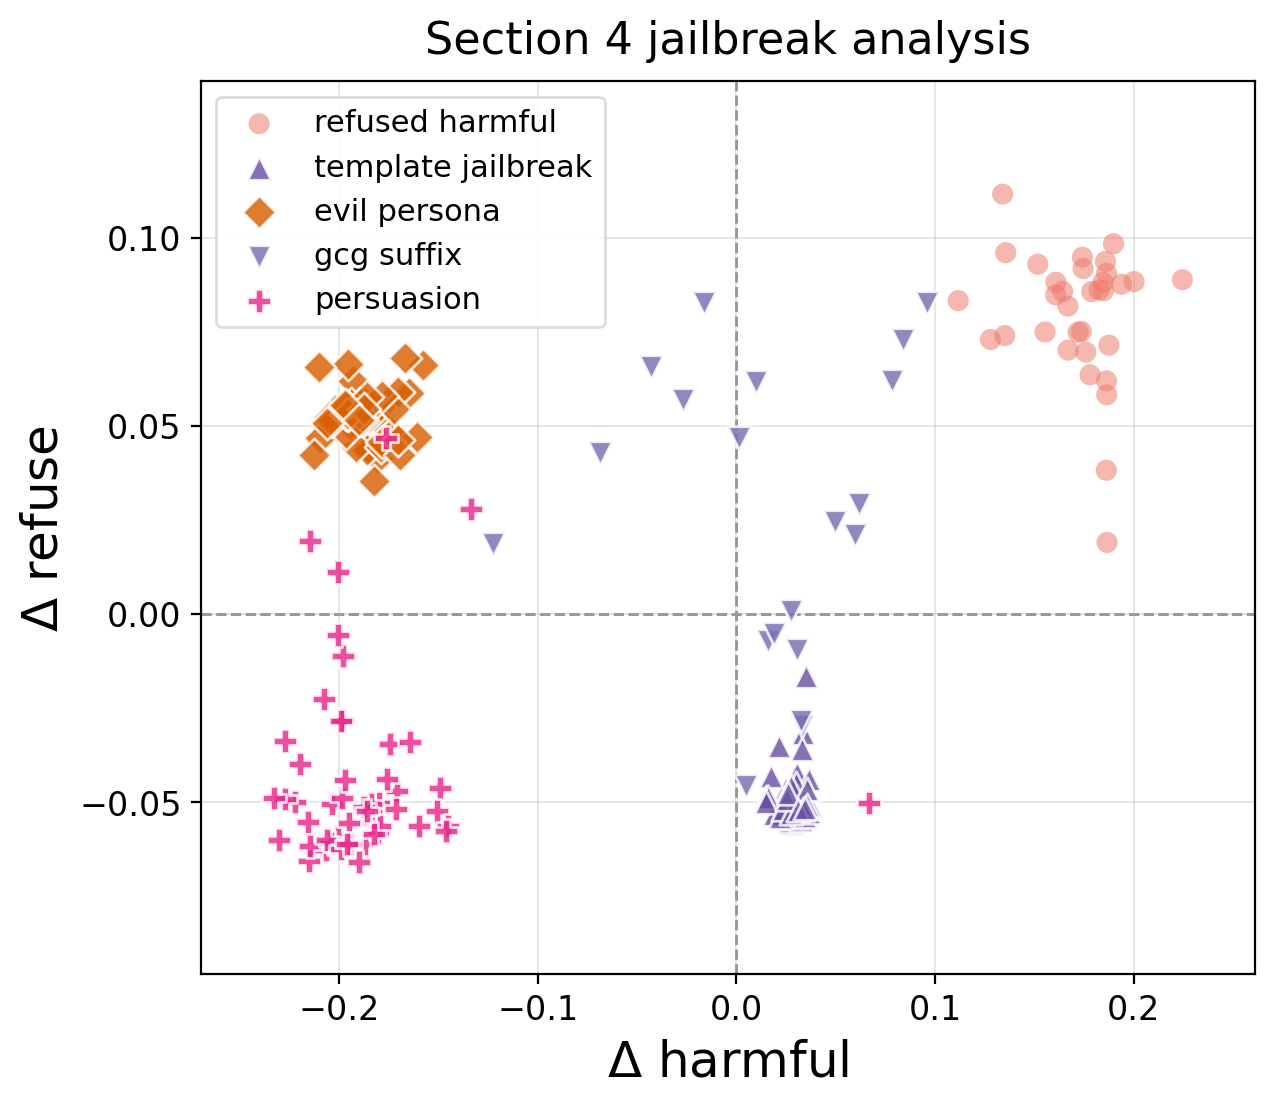
\includegraphics[width=0.72\textwidth]{figures/section4_jailbreak_scatter.png}
\caption{Exploratory jailbreak geometry for Qwen-7B. Refused-harmful baseline prompts are plotted alongside template jailbreaks, evil-persona prompts, GCG suffixes, and persuasion prompts. The attack families occupy distinct regions of the harmfulness/refusal plane.}
\label{fig:appendix-jailbreak-scatter}
\end{figure*}

\begin{table}[t]
\caption{Heuristic harmful-compliance audit for the jailbreak prompt families in \cref{fig:appendix-jailbreak-scatter}. The evaluator separates explicit refusals, benign diversions, and responses that appear to continue addressing the original harmful request. These labels are a sanity-check audit rather than a substitute for human or LLM judging.}
\label{tab:appendix-compliance}
\vskip 0.08in
\centering
\begin{small}
\resizebox{\columnwidth}{!}{%
\begin{tabular}{lrrrr}
\toprule
Prompt family & $n$ & Refusal & Benign & Harmful \\
\midrule
Evil persona & 50 & 50 & 0 & 0 \\
GCG suffix & 20 & 15 & 4 & 1 \\
GPTFuzzer/template & 50 & 0 & 23 & 27 \\
Persuasion & 50 & 8 & 31 & 11 \\
\bottomrule
\end{tabular}
}
\end{small}
\vskip -0.08in
\end{table}

\subsection{CoT-Length and Projection Diagnostics}
\label{sec:appendix-cot-probes}

We also include an exploratory layer sweep from a separate Qwen3-thinking probe. For each intervened layer, we measured whether a chain of thought was produced, its length, and projection scores onto harmfulness/refusal directions at $t_{\text{inst}}$ and $t_{\text{post-inst}}$. This diagnostic complements the main token-slot analysis by showing how inversion-style interventions co-vary with both CoT length and layer-wise projection scores. In the summarized runs, non-inversion settings produce longer CoTs on average, while inversion settings shorten the reasoning trace for both harmfulness and refusal probes. This gives a direct way to connect activation steering, reasoning length, and the internal harmfulness/refusal coordinates.

\begin{figure*}[t]
\centering
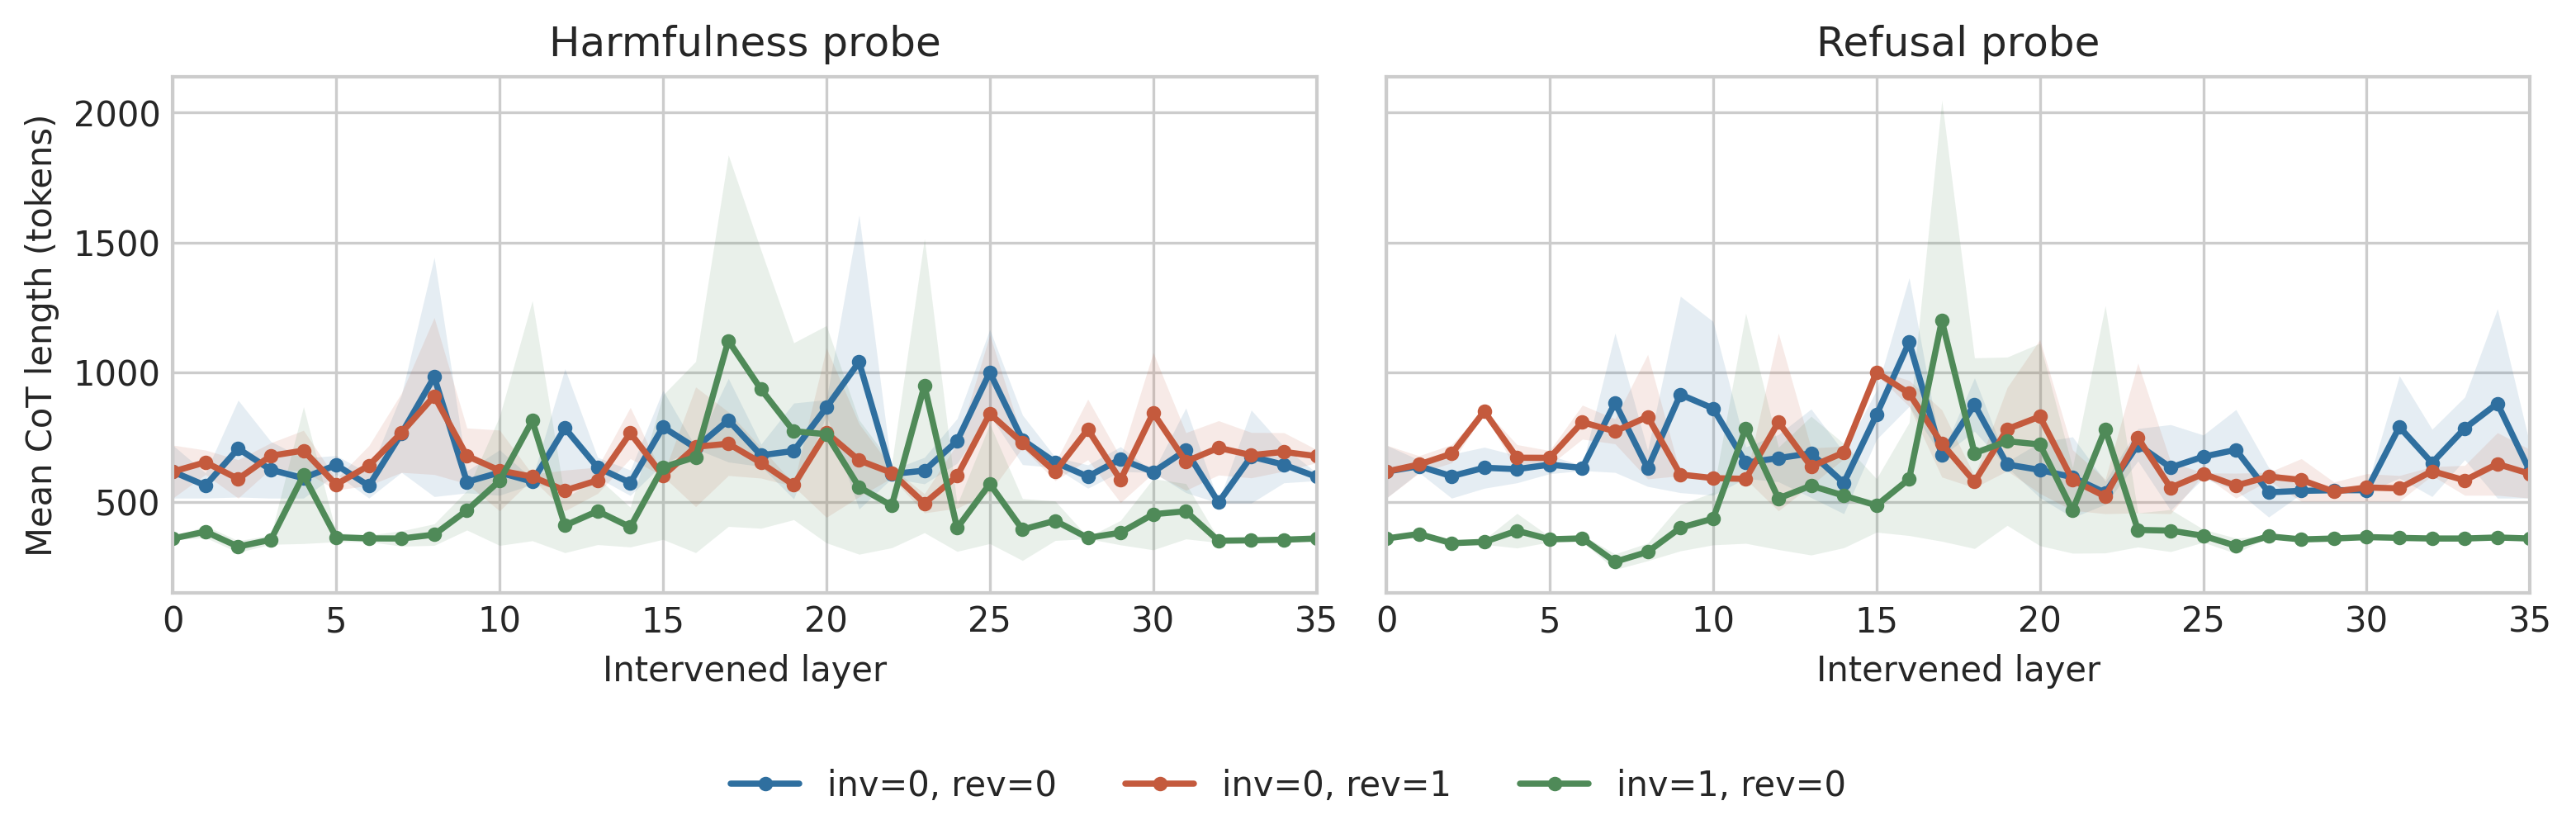
\includegraphics[width=0.95\textwidth]{figures/data_probe_cot_length.png}
\caption{Exploratory CoT-length diagnostics under inversion and non-inversion settings. Inversion settings produce shorter CoTs on average than non-inversion settings for both harmfulness and refusal probes.}
\label{fig:appendix-cot-length}
\end{figure*}

\begin{figure*}[t]
\centering
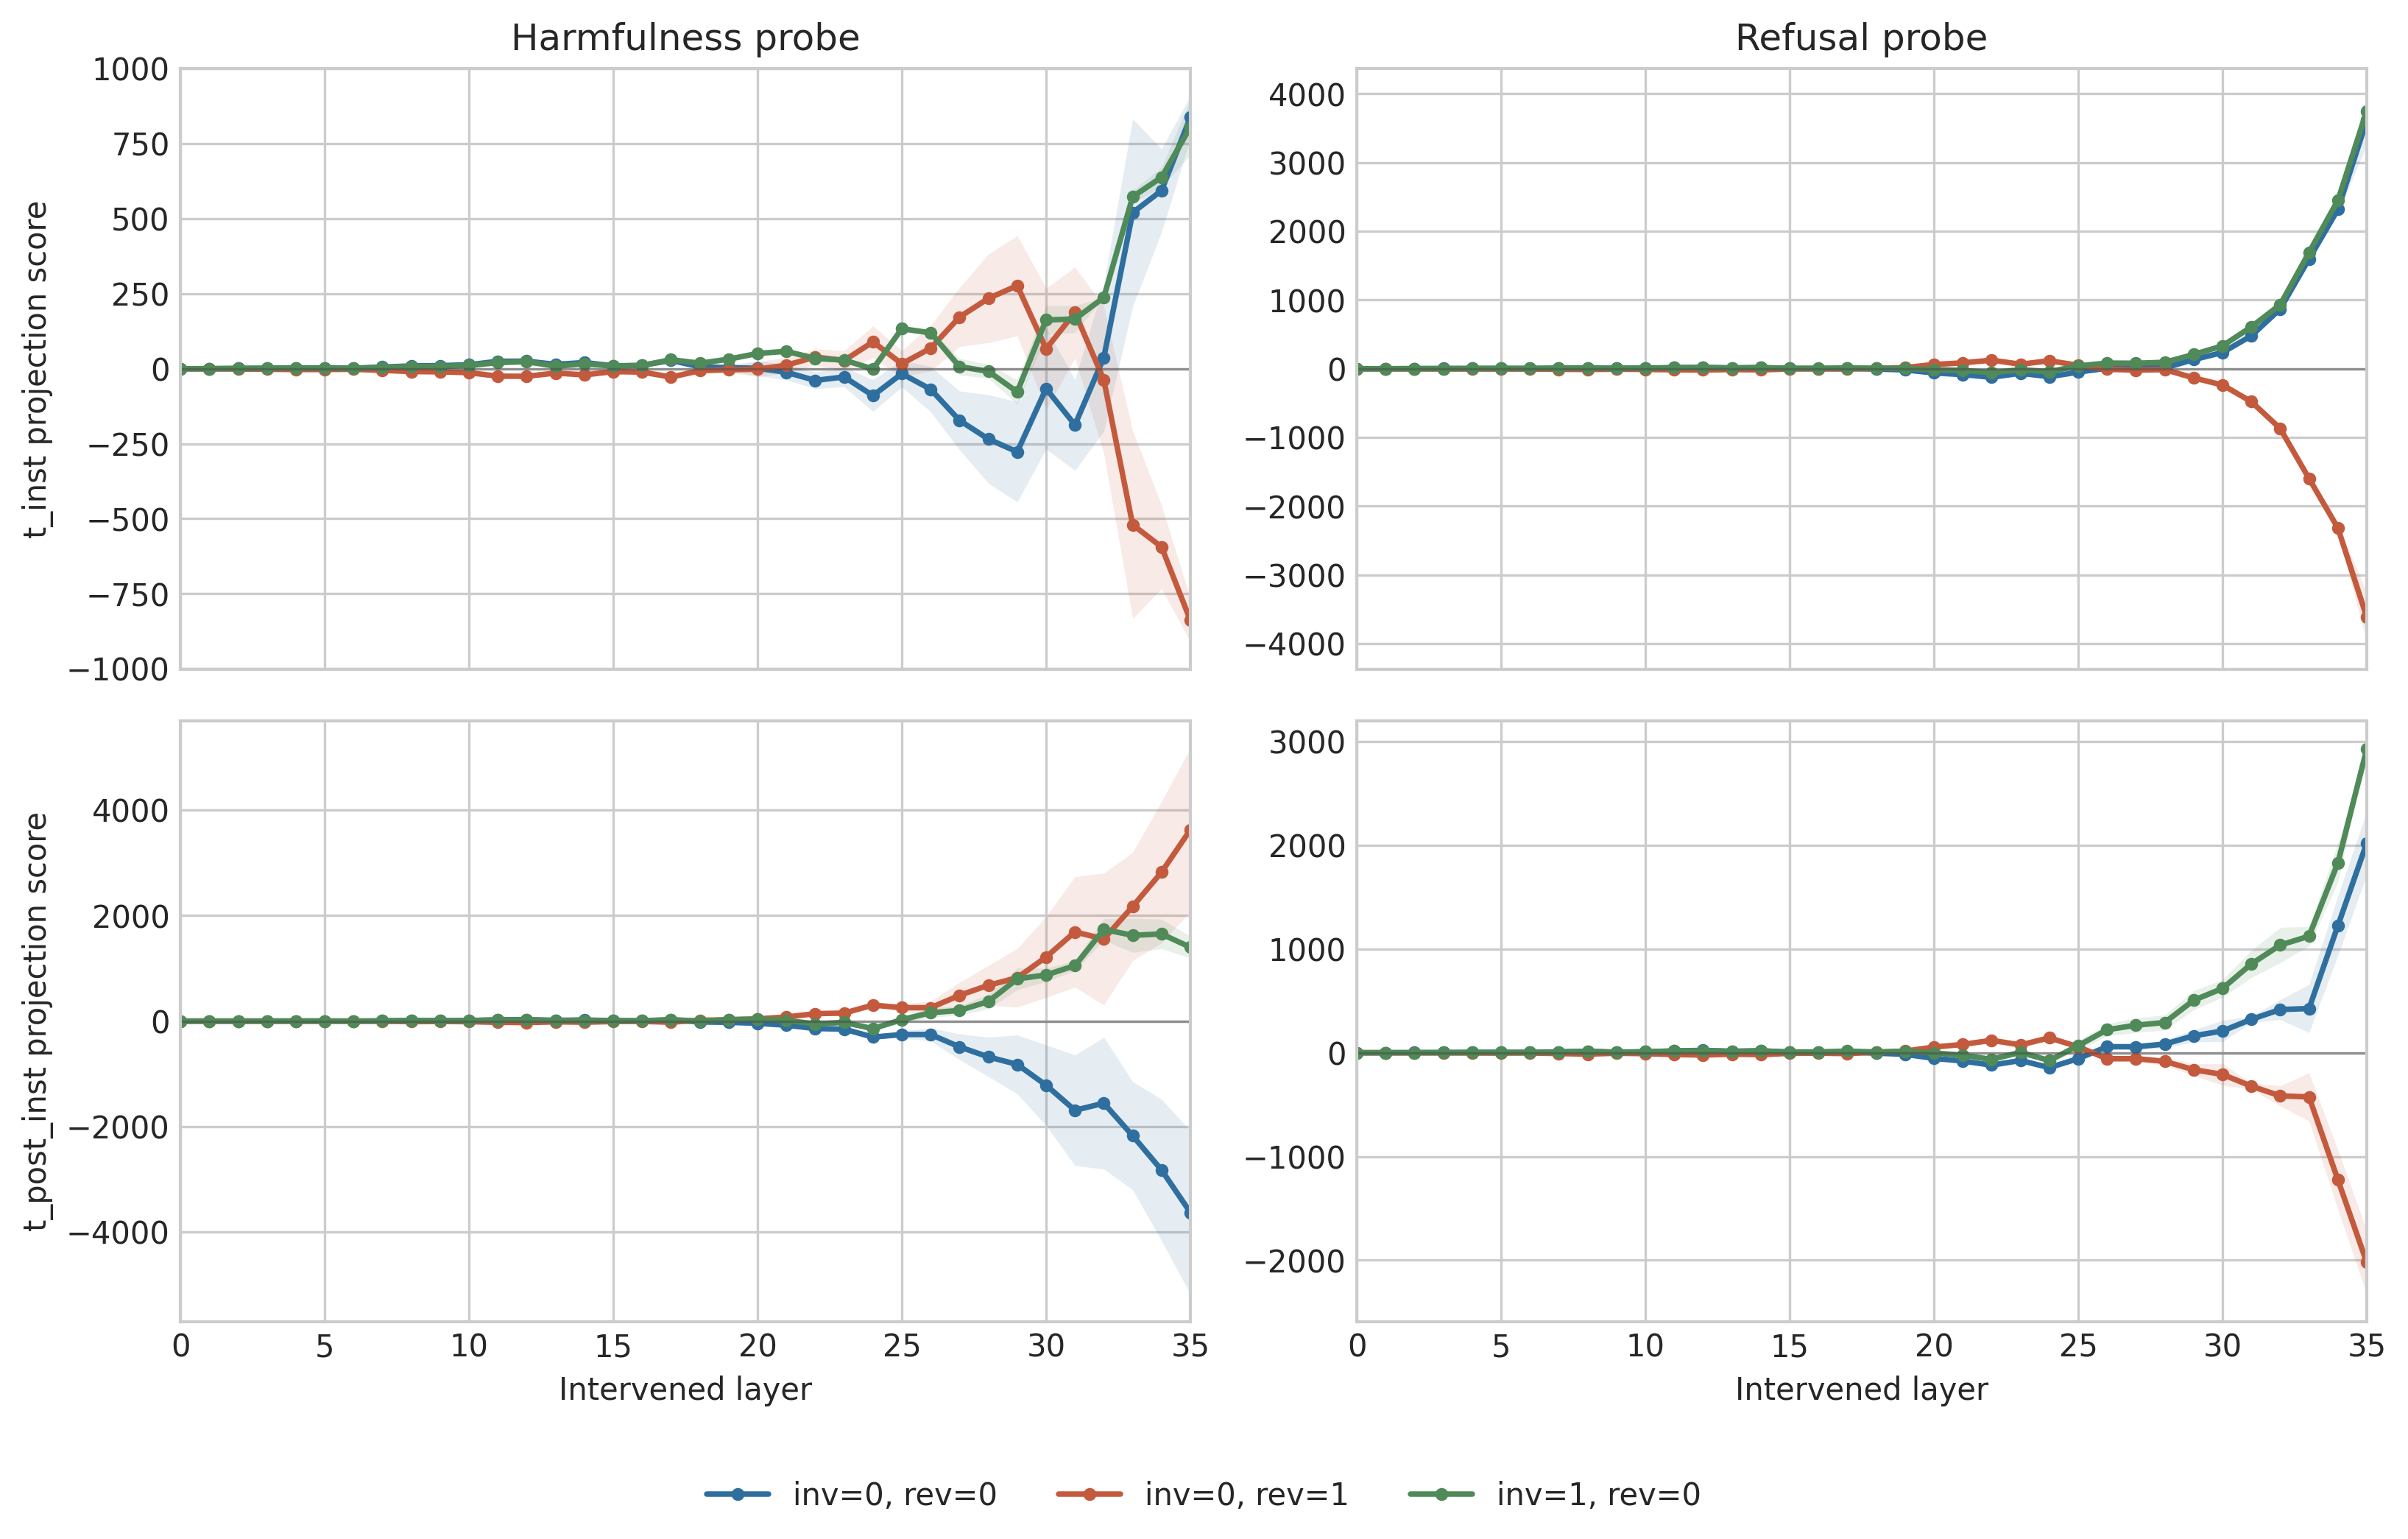
\includegraphics[width=0.95\textwidth]{figures/data_probe_layer_sweep.png}
\caption{Exploratory projection-score layer sweep for harmfulness and refusal probes. Scores vary strongly by layer, especially in later layers, suggesting that steering effects are layer-dependent rather than uniform across the network.}
\label{fig:appendix-projection-sweep}
\end{figure*}

\end{document}